\documentclass[
    %iai, % Saisir le nom de l'institut rattaché
    mi, % Saisir le nom de l'orientation
    %confidential, % Décommentez si le travail est confidentiel
,table]{heig-tb}

\usepackage[nooldvoltagedirection,european,americaninductors]{circuitikz}
\usepackage[T1]{fontenc}
\usepackage{xcolor}
\usepackage{hyperref}

\usepackage[
    left = \flqq{},%
    right = \frqq{},%
    leftsub = \flq{},%
    rightsub = \frq{} %
]{dirtytalk}

\usepackage{subcaption}
\usepackage{pdfpages}
\usepackage{matlab-prettifier}
%\usepackage{biblatex}

\signature{mbernasconi.svg} % Remplacer par votre propre signature vectorielle.

\makenomenclature
\makenoidxglossaries
\makeindex

\addbibresource{bibliography.bib}

\input{nomenclature}
\input{acronyms}
\input{glossary}
% Auteur du document (étudiant-e) en projet de Bachelor
\author{Antoine Oberson}

% Activer l'option pour l'accord du féminin dans le texte
%\genre{female}

% Titre de votre travail de Bachelor
\title{Rapport de travail de Bachelor}

% Le sous titre est optionnel
\subtitle{Générateur de turbulence optique pour le test de systèmes de propagation de faisceau à travers l'atmosphère terrestre}


% Nom du professeur responsable
\teacher {Prof. Jolissaint Laurent(HEIG-VD)}

% Mettre à jour avec la date de rendu du travail
\date{\today}

% Numéro de TB
\thesis{7212}



\surroundwithmdframed{minted}

%% Début du document
%%%%%%%%%%%%%%%%%%%%%%%%%%%%%%%%%%%%%%%%%%%%%%%%%%%%%%%%%%%%%%%%%%%%%%%%%%%%%%%% 
%%% ~ Arduino Language - Arduino IDE Colors ~                                  %%%
%%%                                                                            %%%
%%% Kyle Rocha-Brownell | 10/2/2017 | No Licence                               %%%
%%% -------------------------------------------------------------------------- %%%
%%%                                                                            %%%
%%% Place this file in your working directory (next to the latex file you're   %%%
%%% working on).  To add it to your project, place:                            %%%
%%%    %%%%%%%%%%%%%%%%%%%%%%%%%%%%%%%%%%%%%%%%%%%%%%%%%%%%%%%%%%%%%%%%%%%%%%%%%%%%%%%% 
%%% ~ Arduino Language - Arduino IDE Colors ~                                  %%%
%%%                                                                            %%%
%%% Kyle Rocha-Brownell | 10/2/2017 | No Licence                               %%%
%%% -------------------------------------------------------------------------- %%%
%%%                                                                            %%%
%%% Place this file in your working directory (next to the latex file you're   %%%
%%% working on).  To add it to your project, place:                            %%%
%%%    %%%%%%%%%%%%%%%%%%%%%%%%%%%%%%%%%%%%%%%%%%%%%%%%%%%%%%%%%%%%%%%%%%%%%%%%%%%%%%%% 
%%% ~ Arduino Language - Arduino IDE Colors ~                                  %%%
%%%                                                                            %%%
%%% Kyle Rocha-Brownell | 10/2/2017 | No Licence                               %%%
%%% -------------------------------------------------------------------------- %%%
%%%                                                                            %%%
%%% Place this file in your working directory (next to the latex file you're   %%%
%%% working on).  To add it to your project, place:                            %%%
%%%    \input{arduinoLanguage.tex}                                             %%%
%%% somewhere before \begin{document} in your latex file.                      %%%
%%%                                                                            %%%
%%% In your document, place your arduino code between:                         %%%
%%%   \begin{lstlisting}[language=Arduino]                                     %%%
%%% and:                                                                       %%%
%%%   \end{lstlisting}                                                         %%%
%%%                                                                            %%%
%%% Or create your own style to add non-built-in functions and variables.      %%%
%%%                                                                            %%%
%%%%%%%%%%%%%%%%%%%%%%%%%%%%%%%%%%%%%%%%%%%%%%%%%%%%%%%%%%%%%%%%%%%%%%%%%%%%%%%% 

\usepackage{color}
\usepackage{listings}
\usepackage{courier}

%%% Define Custom IDE Colors %%%
\definecolor{arduinoGreen}    {rgb} {0.17, 0.43, 0.01}
\definecolor{arduinoGrey}     {rgb} {0.47, 0.47, 0.33}
\definecolor{arduinoOrange}   {rgb} {0.8 , 0.4 , 0   }
\definecolor{arduinoBlue}     {rgb} {0.01, 0.61, 0.98}
\definecolor{arduinoDarkBlue} {rgb} {0.0 , 0.2 , 0.5 }

%%% Define Arduino Language %%%
\lstdefinelanguage{Arduino}{
  language=C++, % begin with default C++ settings
  %
  %
  %%% Keyword Color Group 1 %%%  (called KEYWORD3 by arduino)
  keywordstyle=\color{arduinoGreen},
  deletekeywords={  % remove all arduino keywords that might be in c++
      break, case, override, final, continue, default, do, else, for, 
      if, return, goto, switch, throw, try, while, setup, loop, export, 
      not, or, and, xor, include, define, elif, else, error, if, ifdef, 
      ifndef, pragma, warning,
      HIGH, LOW, INPUT, INPUT_PULLUP, OUTPUT, DEC, BIN, HEX, OCT, PI, 
      HALF_PI, TWO_PI, LSBFIRST, MSBFIRST, CHANGE, FALLING, RISING, 
      DEFAULT, EXTERNAL, INTERNAL, INTERNAL1V1, INTERNAL2V56, LED_BUILTIN, 
      LED_BUILTIN_RX, LED_BUILTIN_TX, DIGITAL_MESSAGE, FIRMATA_STRING, 
      ANALOG_MESSAGE, REPORT_DIGITAL, REPORT_ANALOG, SET_PIN_MODE, 
      SYSTEM_RESET, SYSEX_START, auto, int8_t, int16_t, int32_t, int64_t, 
      uint8_t, uint16_t, uint32_t, uint64_t, char16_t, char32_t, operator, 
      enum, delete, bool, boolean, byte, char, const, false, float, double, 
      null, NULL, int, long, new, private, protected, public, short, 
      signed, static, volatile, String, void, true, unsigned, word, array, 
      sizeof, dynamic_cast, typedef, const_cast, struct, static_cast, union, 
      friend, extern, class, reinterpret_cast, register, explicit, inline, 
      _Bool, complex, _Complex, _Imaginary, atomic_bool, atomic_char, 
      atomic_schar, atomic_uchar, atomic_short, atomic_ushort, atomic_int, 
      atomic_uint, atomic_long, atomic_ulong, atomic_llong, atomic_ullong, 
      virtual, PROGMEM,
      Serial, Serial1, Serial2, Serial3, SerialUSB, Keyboard, Mouse,
      abs, acos, asin, atan, atan2, ceil, constrain, cos, degrees, exp, 
      floor, log, map, max, min, radians, random, randomSeed, round, sin, 
      sq, sqrt, tan, pow, bitRead, bitWrite, bitSet, bitClear, bit, 
      highByte, lowByte, analogReference, analogRead, 
      analogReadResolution, analogWrite, analogWriteResolution, 
      attachInterrupt, detachInterrupt, digitalPinToInterrupt, delay, 
      delayMicroseconds, digitalWrite, digitalRead, interrupts, millis, 
      micros, noInterrupts, noTone, pinMode, pulseIn, pulseInLong, shiftIn, 
      shiftOut, tone, yield, Stream, begin, end, peek, read, print, 
      println, available, availableForWrite, flush, setTimeout, find, 
      findUntil, parseInt, parseFloat, readBytes, readBytesUntil, readString, 
      readStringUntil, trim, toUpperCase, toLowerCase, charAt, compareTo, 
      concat, endsWith, startsWith, equals, equalsIgnoreCase, getBytes, 
      indexOf, lastIndexOf, length, replace, setCharAt, substring, 
      toCharArray, toInt, press, release, releaseAll, accept, click, move, 
      isPressed, isAlphaNumeric, isAlpha, isAscii, isWhitespace, isControl, 
      isDigit, isGraph, isLowerCase, isPrintable, isPunct, isSpace, 
      isUpperCase, isHexadecimalDigit, 
    }, 
  morekeywords={   % add arduino structures to group 1
      break, case, override, final, continue, default, do, else, for, 
      if, return, goto, switch, throw, try, while, setup, loop, export, 
      not, or, and, xor, include, define, elif, else, error, if, ifdef, 
      ifndef, pragma, warning,
    }, 
  % 
  %
  %%% Keyword Color Group 2 %%%  (called LITERAL1 by arduino)
  keywordstyle=[2]\color{arduinoBlue},   
  keywords=[2]{   % add variables and dataTypes as 2nd group  
      HIGH, LOW, INPUT, INPUT_PULLUP, OUTPUT, DEC, BIN, HEX, OCT, PI, 
      HALF_PI, TWO_PI, LSBFIRST, MSBFIRST, CHANGE, FALLING, RISING, 
      DEFAULT, EXTERNAL, INTERNAL, INTERNAL1V1, INTERNAL2V56, LED_BUILTIN, 
      LED_BUILTIN_RX, LED_BUILTIN_TX, DIGITAL_MESSAGE, FIRMATA_STRING, 
      ANALOG_MESSAGE, REPORT_DIGITAL, REPORT_ANALOG, SET_PIN_MODE, 
      SYSTEM_RESET, SYSEX_START, auto, int8_t, int16_t, int32_t, int64_t, 
      uint8_t, uint16_t, uint32_t, uint64_t, char16_t, char32_t, operator, 
      enum, delete, bool, boolean, byte, char, const, false, float, double, 
      null, NULL, int, long, new, private, protected, public, short, 
      signed, static, volatile, String, void, true, unsigned, word, array, 
      sizeof, dynamic_cast, typedef, const_cast, struct, static_cast, union, 
      friend, extern, class, reinterpret_cast, register, explicit, inline, 
      _Bool, complex, _Complex, _Imaginary, atomic_bool, atomic_char, 
      atomic_schar, atomic_uchar, atomic_short, atomic_ushort, atomic_int, 
      atomic_uint, atomic_long, atomic_ulong, atomic_llong, atomic_ullong, 
      virtual, PROGMEM,
    },  
  % 
  %
  %%% Keyword Color Group 3 %%%  (called KEYWORD1 by arduino)
  keywordstyle=[3]\bfseries\color{arduinoOrange},
  keywords=[3]{  % add built-in functions as a 3rd group
      Serial, Serial1, Serial2, Serial3, SerialUSB, Keyboard, Mouse,
    },      
  %
  %
  %%% Keyword Color Group 4 %%%  (called KEYWORD2 by arduino)
  keywordstyle=[4]\color{arduinoOrange},
  keywords=[4]{  % add more built-in functions as a 4th group
      abs, acos, asin, atan, atan2, ceil, constrain, cos, degrees, exp, 
      floor, log, map, max, min, radians, random, randomSeed, round, sin, 
      sq, sqrt, tan, pow, bitRead, bitWrite, bitSet, bitClear, bit, 
      highByte, lowByte, analogReference, analogRead, 
      analogReadResolution, analogWrite, analogWriteResolution, 
      attachInterrupt, detachInterrupt, digitalPinToInterrupt, delay, 
      delayMicroseconds, digitalWrite, digitalRead, interrupts, millis, 
      micros, noInterrupts, noTone, pinMode, pulseIn, pulseInLong, shiftIn, 
      shiftOut, tone, yield, Stream, begin, end, peek, read, print, 
      println, available, availableForWrite, flush, setTimeout, find, 
      findUntil, parseInt, parseFloat, readBytes, readBytesUntil, readString, 
      readStringUntil, trim, toUpperCase, toLowerCase, charAt, compareTo, 
      concat, endsWith, startsWith, equals, equalsIgnoreCase, getBytes, 
      indexOf, lastIndexOf, length, replace, setCharAt, substring, 
      toCharArray, toInt, press, release, releaseAll, accept, click, move, 
      isPressed, isAlphaNumeric, isAlpha, isAscii, isWhitespace, isControl, 
      isDigit, isGraph, isLowerCase, isPrintable, isPunct, isSpace, 
      isUpperCase, isHexadecimalDigit, 
    },      
  %
  %
  %%% Set Other Colors %%%
  stringstyle=\color{arduinoDarkBlue},    
  commentstyle=\color{arduinoGrey},    
  %          
  %   
  %%%% Line Numbering %%%%
  numbers=left,                    
  numbersep=5pt,                   
  numberstyle=\color{arduinoGrey},    
  %stepnumber=2,                      % show every 2 line numbers
  %
  %
  %%%% Code Box Style %%%%
  breaklines=true,                    % wordwrapping
  tabsize=2,         
  basicstyle=\ttfamily  
}
                                             %%%
%%% somewhere before \begin{document} in your latex file.                      %%%
%%%                                                                            %%%
%%% In your document, place your arduino code between:                         %%%
%%%   \begin{lstlisting}[language=Arduino]                                     %%%
%%% and:                                                                       %%%
%%%   \end{lstlisting}                                                         %%%
%%%                                                                            %%%
%%% Or create your own style to add non-built-in functions and variables.      %%%
%%%                                                                            %%%
%%%%%%%%%%%%%%%%%%%%%%%%%%%%%%%%%%%%%%%%%%%%%%%%%%%%%%%%%%%%%%%%%%%%%%%%%%%%%%%% 

\usepackage{color}
\usepackage{listings}
\usepackage{courier}

%%% Define Custom IDE Colors %%%
\definecolor{arduinoGreen}    {rgb} {0.17, 0.43, 0.01}
\definecolor{arduinoGrey}     {rgb} {0.47, 0.47, 0.33}
\definecolor{arduinoOrange}   {rgb} {0.8 , 0.4 , 0   }
\definecolor{arduinoBlue}     {rgb} {0.01, 0.61, 0.98}
\definecolor{arduinoDarkBlue} {rgb} {0.0 , 0.2 , 0.5 }

%%% Define Arduino Language %%%
\lstdefinelanguage{Arduino}{
  language=C++, % begin with default C++ settings
  %
  %
  %%% Keyword Color Group 1 %%%  (called KEYWORD3 by arduino)
  keywordstyle=\color{arduinoGreen},
  deletekeywords={  % remove all arduino keywords that might be in c++
      break, case, override, final, continue, default, do, else, for, 
      if, return, goto, switch, throw, try, while, setup, loop, export, 
      not, or, and, xor, include, define, elif, else, error, if, ifdef, 
      ifndef, pragma, warning,
      HIGH, LOW, INPUT, INPUT_PULLUP, OUTPUT, DEC, BIN, HEX, OCT, PI, 
      HALF_PI, TWO_PI, LSBFIRST, MSBFIRST, CHANGE, FALLING, RISING, 
      DEFAULT, EXTERNAL, INTERNAL, INTERNAL1V1, INTERNAL2V56, LED_BUILTIN, 
      LED_BUILTIN_RX, LED_BUILTIN_TX, DIGITAL_MESSAGE, FIRMATA_STRING, 
      ANALOG_MESSAGE, REPORT_DIGITAL, REPORT_ANALOG, SET_PIN_MODE, 
      SYSTEM_RESET, SYSEX_START, auto, int8_t, int16_t, int32_t, int64_t, 
      uint8_t, uint16_t, uint32_t, uint64_t, char16_t, char32_t, operator, 
      enum, delete, bool, boolean, byte, char, const, false, float, double, 
      null, NULL, int, long, new, private, protected, public, short, 
      signed, static, volatile, String, void, true, unsigned, word, array, 
      sizeof, dynamic_cast, typedef, const_cast, struct, static_cast, union, 
      friend, extern, class, reinterpret_cast, register, explicit, inline, 
      _Bool, complex, _Complex, _Imaginary, atomic_bool, atomic_char, 
      atomic_schar, atomic_uchar, atomic_short, atomic_ushort, atomic_int, 
      atomic_uint, atomic_long, atomic_ulong, atomic_llong, atomic_ullong, 
      virtual, PROGMEM,
      Serial, Serial1, Serial2, Serial3, SerialUSB, Keyboard, Mouse,
      abs, acos, asin, atan, atan2, ceil, constrain, cos, degrees, exp, 
      floor, log, map, max, min, radians, random, randomSeed, round, sin, 
      sq, sqrt, tan, pow, bitRead, bitWrite, bitSet, bitClear, bit, 
      highByte, lowByte, analogReference, analogRead, 
      analogReadResolution, analogWrite, analogWriteResolution, 
      attachInterrupt, detachInterrupt, digitalPinToInterrupt, delay, 
      delayMicroseconds, digitalWrite, digitalRead, interrupts, millis, 
      micros, noInterrupts, noTone, pinMode, pulseIn, pulseInLong, shiftIn, 
      shiftOut, tone, yield, Stream, begin, end, peek, read, print, 
      println, available, availableForWrite, flush, setTimeout, find, 
      findUntil, parseInt, parseFloat, readBytes, readBytesUntil, readString, 
      readStringUntil, trim, toUpperCase, toLowerCase, charAt, compareTo, 
      concat, endsWith, startsWith, equals, equalsIgnoreCase, getBytes, 
      indexOf, lastIndexOf, length, replace, setCharAt, substring, 
      toCharArray, toInt, press, release, releaseAll, accept, click, move, 
      isPressed, isAlphaNumeric, isAlpha, isAscii, isWhitespace, isControl, 
      isDigit, isGraph, isLowerCase, isPrintable, isPunct, isSpace, 
      isUpperCase, isHexadecimalDigit, 
    }, 
  morekeywords={   % add arduino structures to group 1
      break, case, override, final, continue, default, do, else, for, 
      if, return, goto, switch, throw, try, while, setup, loop, export, 
      not, or, and, xor, include, define, elif, else, error, if, ifdef, 
      ifndef, pragma, warning,
    }, 
  % 
  %
  %%% Keyword Color Group 2 %%%  (called LITERAL1 by arduino)
  keywordstyle=[2]\color{arduinoBlue},   
  keywords=[2]{   % add variables and dataTypes as 2nd group  
      HIGH, LOW, INPUT, INPUT_PULLUP, OUTPUT, DEC, BIN, HEX, OCT, PI, 
      HALF_PI, TWO_PI, LSBFIRST, MSBFIRST, CHANGE, FALLING, RISING, 
      DEFAULT, EXTERNAL, INTERNAL, INTERNAL1V1, INTERNAL2V56, LED_BUILTIN, 
      LED_BUILTIN_RX, LED_BUILTIN_TX, DIGITAL_MESSAGE, FIRMATA_STRING, 
      ANALOG_MESSAGE, REPORT_DIGITAL, REPORT_ANALOG, SET_PIN_MODE, 
      SYSTEM_RESET, SYSEX_START, auto, int8_t, int16_t, int32_t, int64_t, 
      uint8_t, uint16_t, uint32_t, uint64_t, char16_t, char32_t, operator, 
      enum, delete, bool, boolean, byte, char, const, false, float, double, 
      null, NULL, int, long, new, private, protected, public, short, 
      signed, static, volatile, String, void, true, unsigned, word, array, 
      sizeof, dynamic_cast, typedef, const_cast, struct, static_cast, union, 
      friend, extern, class, reinterpret_cast, register, explicit, inline, 
      _Bool, complex, _Complex, _Imaginary, atomic_bool, atomic_char, 
      atomic_schar, atomic_uchar, atomic_short, atomic_ushort, atomic_int, 
      atomic_uint, atomic_long, atomic_ulong, atomic_llong, atomic_ullong, 
      virtual, PROGMEM,
    },  
  % 
  %
  %%% Keyword Color Group 3 %%%  (called KEYWORD1 by arduino)
  keywordstyle=[3]\bfseries\color{arduinoOrange},
  keywords=[3]{  % add built-in functions as a 3rd group
      Serial, Serial1, Serial2, Serial3, SerialUSB, Keyboard, Mouse,
    },      
  %
  %
  %%% Keyword Color Group 4 %%%  (called KEYWORD2 by arduino)
  keywordstyle=[4]\color{arduinoOrange},
  keywords=[4]{  % add more built-in functions as a 4th group
      abs, acos, asin, atan, atan2, ceil, constrain, cos, degrees, exp, 
      floor, log, map, max, min, radians, random, randomSeed, round, sin, 
      sq, sqrt, tan, pow, bitRead, bitWrite, bitSet, bitClear, bit, 
      highByte, lowByte, analogReference, analogRead, 
      analogReadResolution, analogWrite, analogWriteResolution, 
      attachInterrupt, detachInterrupt, digitalPinToInterrupt, delay, 
      delayMicroseconds, digitalWrite, digitalRead, interrupts, millis, 
      micros, noInterrupts, noTone, pinMode, pulseIn, pulseInLong, shiftIn, 
      shiftOut, tone, yield, Stream, begin, end, peek, read, print, 
      println, available, availableForWrite, flush, setTimeout, find, 
      findUntil, parseInt, parseFloat, readBytes, readBytesUntil, readString, 
      readStringUntil, trim, toUpperCase, toLowerCase, charAt, compareTo, 
      concat, endsWith, startsWith, equals, equalsIgnoreCase, getBytes, 
      indexOf, lastIndexOf, length, replace, setCharAt, substring, 
      toCharArray, toInt, press, release, releaseAll, accept, click, move, 
      isPressed, isAlphaNumeric, isAlpha, isAscii, isWhitespace, isControl, 
      isDigit, isGraph, isLowerCase, isPrintable, isPunct, isSpace, 
      isUpperCase, isHexadecimalDigit, 
    },      
  %
  %
  %%% Set Other Colors %%%
  stringstyle=\color{arduinoDarkBlue},    
  commentstyle=\color{arduinoGrey},    
  %          
  %   
  %%%% Line Numbering %%%%
  numbers=left,                    
  numbersep=5pt,                   
  numberstyle=\color{arduinoGrey},    
  %stepnumber=2,                      % show every 2 line numbers
  %
  %
  %%%% Code Box Style %%%%
  breaklines=true,                    % wordwrapping
  tabsize=2,         
  basicstyle=\ttfamily  
}
                                             %%%
%%% somewhere before \begin{document} in your latex file.                      %%%
%%%                                                                            %%%
%%% In your document, place your arduino code between:                         %%%
%%%   \begin{lstlisting}[language=Arduino]                                     %%%
%%% and:                                                                       %%%
%%%   \end{lstlisting}                                                         %%%
%%%                                                                            %%%
%%% Or create your own style to add non-built-in functions and variables.      %%%
%%%                                                                            %%%
%%%%%%%%%%%%%%%%%%%%%%%%%%%%%%%%%%%%%%%%%%%%%%%%%%%%%%%%%%%%%%%%%%%%%%%%%%%%%%%% 

\usepackage{color}
\usepackage{listings}
\usepackage{courier}

%%% Define Custom IDE Colors %%%
\definecolor{arduinoGreen}    {rgb} {0.17, 0.43, 0.01}
\definecolor{arduinoGrey}     {rgb} {0.47, 0.47, 0.33}
\definecolor{arduinoOrange}   {rgb} {0.8 , 0.4 , 0   }
\definecolor{arduinoBlue}     {rgb} {0.01, 0.61, 0.98}
\definecolor{arduinoDarkBlue} {rgb} {0.0 , 0.2 , 0.5 }

%%% Define Arduino Language %%%
\lstdefinelanguage{Arduino}{
  language=C++, % begin with default C++ settings
  %
  %
  %%% Keyword Color Group 1 %%%  (called KEYWORD3 by arduino)
  keywordstyle=\color{arduinoGreen},
  deletekeywords={  % remove all arduino keywords that might be in c++
      break, case, override, final, continue, default, do, else, for, 
      if, return, goto, switch, throw, try, while, setup, loop, export, 
      not, or, and, xor, include, define, elif, else, error, if, ifdef, 
      ifndef, pragma, warning,
      HIGH, LOW, INPUT, INPUT_PULLUP, OUTPUT, DEC, BIN, HEX, OCT, PI, 
      HALF_PI, TWO_PI, LSBFIRST, MSBFIRST, CHANGE, FALLING, RISING, 
      DEFAULT, EXTERNAL, INTERNAL, INTERNAL1V1, INTERNAL2V56, LED_BUILTIN, 
      LED_BUILTIN_RX, LED_BUILTIN_TX, DIGITAL_MESSAGE, FIRMATA_STRING, 
      ANALOG_MESSAGE, REPORT_DIGITAL, REPORT_ANALOG, SET_PIN_MODE, 
      SYSTEM_RESET, SYSEX_START, auto, int8_t, int16_t, int32_t, int64_t, 
      uint8_t, uint16_t, uint32_t, uint64_t, char16_t, char32_t, operator, 
      enum, delete, bool, boolean, byte, char, const, false, float, double, 
      null, NULL, int, long, new, private, protected, public, short, 
      signed, static, volatile, String, void, true, unsigned, word, array, 
      sizeof, dynamic_cast, typedef, const_cast, struct, static_cast, union, 
      friend, extern, class, reinterpret_cast, register, explicit, inline, 
      _Bool, complex, _Complex, _Imaginary, atomic_bool, atomic_char, 
      atomic_schar, atomic_uchar, atomic_short, atomic_ushort, atomic_int, 
      atomic_uint, atomic_long, atomic_ulong, atomic_llong, atomic_ullong, 
      virtual, PROGMEM,
      Serial, Serial1, Serial2, Serial3, SerialUSB, Keyboard, Mouse,
      abs, acos, asin, atan, atan2, ceil, constrain, cos, degrees, exp, 
      floor, log, map, max, min, radians, random, randomSeed, round, sin, 
      sq, sqrt, tan, pow, bitRead, bitWrite, bitSet, bitClear, bit, 
      highByte, lowByte, analogReference, analogRead, 
      analogReadResolution, analogWrite, analogWriteResolution, 
      attachInterrupt, detachInterrupt, digitalPinToInterrupt, delay, 
      delayMicroseconds, digitalWrite, digitalRead, interrupts, millis, 
      micros, noInterrupts, noTone, pinMode, pulseIn, pulseInLong, shiftIn, 
      shiftOut, tone, yield, Stream, begin, end, peek, read, print, 
      println, available, availableForWrite, flush, setTimeout, find, 
      findUntil, parseInt, parseFloat, readBytes, readBytesUntil, readString, 
      readStringUntil, trim, toUpperCase, toLowerCase, charAt, compareTo, 
      concat, endsWith, startsWith, equals, equalsIgnoreCase, getBytes, 
      indexOf, lastIndexOf, length, replace, setCharAt, substring, 
      toCharArray, toInt, press, release, releaseAll, accept, click, move, 
      isPressed, isAlphaNumeric, isAlpha, isAscii, isWhitespace, isControl, 
      isDigit, isGraph, isLowerCase, isPrintable, isPunct, isSpace, 
      isUpperCase, isHexadecimalDigit, 
    }, 
  morekeywords={   % add arduino structures to group 1
      break, case, override, final, continue, default, do, else, for, 
      if, return, goto, switch, throw, try, while, setup, loop, export, 
      not, or, and, xor, include, define, elif, else, error, if, ifdef, 
      ifndef, pragma, warning,
    }, 
  % 
  %
  %%% Keyword Color Group 2 %%%  (called LITERAL1 by arduino)
  keywordstyle=[2]\color{arduinoBlue},   
  keywords=[2]{   % add variables and dataTypes as 2nd group  
      HIGH, LOW, INPUT, INPUT_PULLUP, OUTPUT, DEC, BIN, HEX, OCT, PI, 
      HALF_PI, TWO_PI, LSBFIRST, MSBFIRST, CHANGE, FALLING, RISING, 
      DEFAULT, EXTERNAL, INTERNAL, INTERNAL1V1, INTERNAL2V56, LED_BUILTIN, 
      LED_BUILTIN_RX, LED_BUILTIN_TX, DIGITAL_MESSAGE, FIRMATA_STRING, 
      ANALOG_MESSAGE, REPORT_DIGITAL, REPORT_ANALOG, SET_PIN_MODE, 
      SYSTEM_RESET, SYSEX_START, auto, int8_t, int16_t, int32_t, int64_t, 
      uint8_t, uint16_t, uint32_t, uint64_t, char16_t, char32_t, operator, 
      enum, delete, bool, boolean, byte, char, const, false, float, double, 
      null, NULL, int, long, new, private, protected, public, short, 
      signed, static, volatile, String, void, true, unsigned, word, array, 
      sizeof, dynamic_cast, typedef, const_cast, struct, static_cast, union, 
      friend, extern, class, reinterpret_cast, register, explicit, inline, 
      _Bool, complex, _Complex, _Imaginary, atomic_bool, atomic_char, 
      atomic_schar, atomic_uchar, atomic_short, atomic_ushort, atomic_int, 
      atomic_uint, atomic_long, atomic_ulong, atomic_llong, atomic_ullong, 
      virtual, PROGMEM,
    },  
  % 
  %
  %%% Keyword Color Group 3 %%%  (called KEYWORD1 by arduino)
  keywordstyle=[3]\bfseries\color{arduinoOrange},
  keywords=[3]{  % add built-in functions as a 3rd group
      Serial, Serial1, Serial2, Serial3, SerialUSB, Keyboard, Mouse,
    },      
  %
  %
  %%% Keyword Color Group 4 %%%  (called KEYWORD2 by arduino)
  keywordstyle=[4]\color{arduinoOrange},
  keywords=[4]{  % add more built-in functions as a 4th group
      abs, acos, asin, atan, atan2, ceil, constrain, cos, degrees, exp, 
      floor, log, map, max, min, radians, random, randomSeed, round, sin, 
      sq, sqrt, tan, pow, bitRead, bitWrite, bitSet, bitClear, bit, 
      highByte, lowByte, analogReference, analogRead, 
      analogReadResolution, analogWrite, analogWriteResolution, 
      attachInterrupt, detachInterrupt, digitalPinToInterrupt, delay, 
      delayMicroseconds, digitalWrite, digitalRead, interrupts, millis, 
      micros, noInterrupts, noTone, pinMode, pulseIn, pulseInLong, shiftIn, 
      shiftOut, tone, yield, Stream, begin, end, peek, read, print, 
      println, available, availableForWrite, flush, setTimeout, find, 
      findUntil, parseInt, parseFloat, readBytes, readBytesUntil, readString, 
      readStringUntil, trim, toUpperCase, toLowerCase, charAt, compareTo, 
      concat, endsWith, startsWith, equals, equalsIgnoreCase, getBytes, 
      indexOf, lastIndexOf, length, replace, setCharAt, substring, 
      toCharArray, toInt, press, release, releaseAll, accept, click, move, 
      isPressed, isAlphaNumeric, isAlpha, isAscii, isWhitespace, isControl, 
      isDigit, isGraph, isLowerCase, isPrintable, isPunct, isSpace, 
      isUpperCase, isHexadecimalDigit, 
    },      
  %
  %
  %%% Set Other Colors %%%
  stringstyle=\color{arduinoDarkBlue},    
  commentstyle=\color{arduinoGrey},    
  %          
  %   
  %%%% Line Numbering %%%%
  numbers=left,                    
  numbersep=5pt,                   
  numberstyle=\color{arduinoGrey},    
  %stepnumber=2,                      % show every 2 line numbers
  %
  %
  %%%% Code Box Style %%%%
  breaklines=true,                    % wordwrapping
  tabsize=2,         
  basicstyle=\ttfamily  
}

\begin{document}

\selectlanguage{french}
\maketitle
\frontmatter
\clearemptydoublepage

%% Requis par les dispositions générales des travaux de Bachelor
\preamble
\authentification
\includepdf[pages=-]{assets/figures/scan_enonce/scan_énoncé.pdf}
% \begin{figure}[H]
%     \centering
%     \includegraphics[page=1-,width = \textwidth]{assets/figures/scan_enonce/scan_énoncé.pdf}
% \end{figure}


%% Résumé / Résumé publiable / Version abrégée
\begin{abstract}
    % Francais
%\lipsum[1]

\asterism

% English
\lipsum[3]

\end{abstract}

%% Sommaire et tables
\clearemptydoublepage
{
    \tableofcontents
    \let\cleardoublepage\clearpage
    \listoffigures
    \let\cleardoublepage\clearpage
    \listoftables
    \let\cleardoublepage\clearpage
    \listoflistings
}

\printnomenclature
\clearemptydoublepage
\pagenumbering{arabic}

\hypersetup{
    colorlinks=true,
    linkcolor=blue,
    filecolor=magenta,
    urlcolor=cyan,
    pdftitle={Overleaf Example},
    pdfpagemode=FullScreen,
}

%% Contenu
\mainmatter
\chapter{Introduction}
%L'introduction est une section requise dans un rapport technique. Introduisez votre travail, l'idée de départ et les objectifs attendus. Un lecteur qui découvrirait votre projet au travers de cette introduction devrait ainsi être capable d'en comprendre le cadre, l'idée générale et les aboutissants du projet.

En 2014, le laboratoire d'optique (Optolab.iai) de l'HEIG-VD a produit le design optique et les instruments de 1ère génération du \href{https://atasam.atauni.edu.tr/}{DAG (Dogu Anadolu Gözlemevi, Eastern Anatolia Observatory)}\footnotemark
un téléscope optique et infrarouge proche de 4m de diamètre situé en Turquie à 3000m d'altitude dans les montagnes Palandöken proche de la ville d'Erzurum en Anatolie de l'est.Plus précisémment aux collines de Karakaya, cette région fut sélectionnée pour sa faible humidité, le vent y est faible et sa direction est stable
,le nombre de jours et nuits clairs, une ville est à proximité mais elle n'est pas visible depuis la localisation du DAG, il y a donc peu de pollution lumineuse, ces caractéristiques atmosphériques et structurelles en font donc un endroit propice à l'installation de plusieur grand téléscope permettant entre autre l'observation
dans l'infrarouge proche (ce qui est possible dans peu d'endroits au monde).

Malheureusement, même avec les conditions atmosphériques et géographiques les plus parfaites, le téléscope fait toujours face à un grand ennemi : \textbf{les turbulences}.
Le travail actuel d'Optolab est donc de développer un système d'optique adaptative ayant pour but de contrer les turbulences optiques produites par l'atmosphère. Ce système
d'optique adaptative a besoin d'être testé à l'aide d'écrans circulaires permettant de simuler des turbulances optiques.

Dans le cadre de ce projet de Bachelor, il convient donc de reprendre le travail réalisé dans un projet de Master précédent de l'HES-SO, ce dernier consistait en une boîte permettant de projeter un gas d'acrylique transparente sur une plaque de plastique, elle aussi, transparente. La turbulence du nuage de gas
d'acrylique immortalise sur la plaque en plastique une différence de chemin optique similaire à la distribution de la turbulence optique.

Le but de ce travail de Bachelor est donc de comprendre le fonctionnement de la machine de projection pour en suite l'améliorer afin de produire in-situ des écrans de phase calibrés.
\footnotetext{\url{https://atasam.atauni.edu.tr/}}

\newpage


\section{Contexte}
Cette section \underline{n'est pas obligatoire}, mais elle est souvent présente dans un rapport technique pour compléter l'introduction et définir le contexte du travail \cad le cadre formel dans lequel le travail est mené.




\chapter{Théorie}
\section{Fondamentaux}
Cette section parcourt les notions fondamentales d'optique pour comprendre la suite de ce rapport.

\subsection{Le seeing astronomique}
Le seeing, de l'anglais du mot vision (plutôt de l'action de voir), est le mot utilisé pour parler de la dégradation de l'image
d'un objet astronomique par les turbulences atmosphériques, plus concrètement cela se traduit pour un effet de flou et de distorsion sur l'image.

L'atmosphère est composée de plusieurs couches d'air aux densités et températures différentes, qui ont pour effet de modifier leurs coefficients de réfraction, la lumière devra donc passer
dans des couches aux indices de réfraction différents, causant alors des réfractions de la lumière non uniformes.

Le seeing peut être quantifié en seconde d'arc du disque de seeing, le diamètre de ce disque est égal à la \textbf{largeur à mis-hauteur} de l'intensité lumineuse :
\begin{figure}[H]
  \centering
  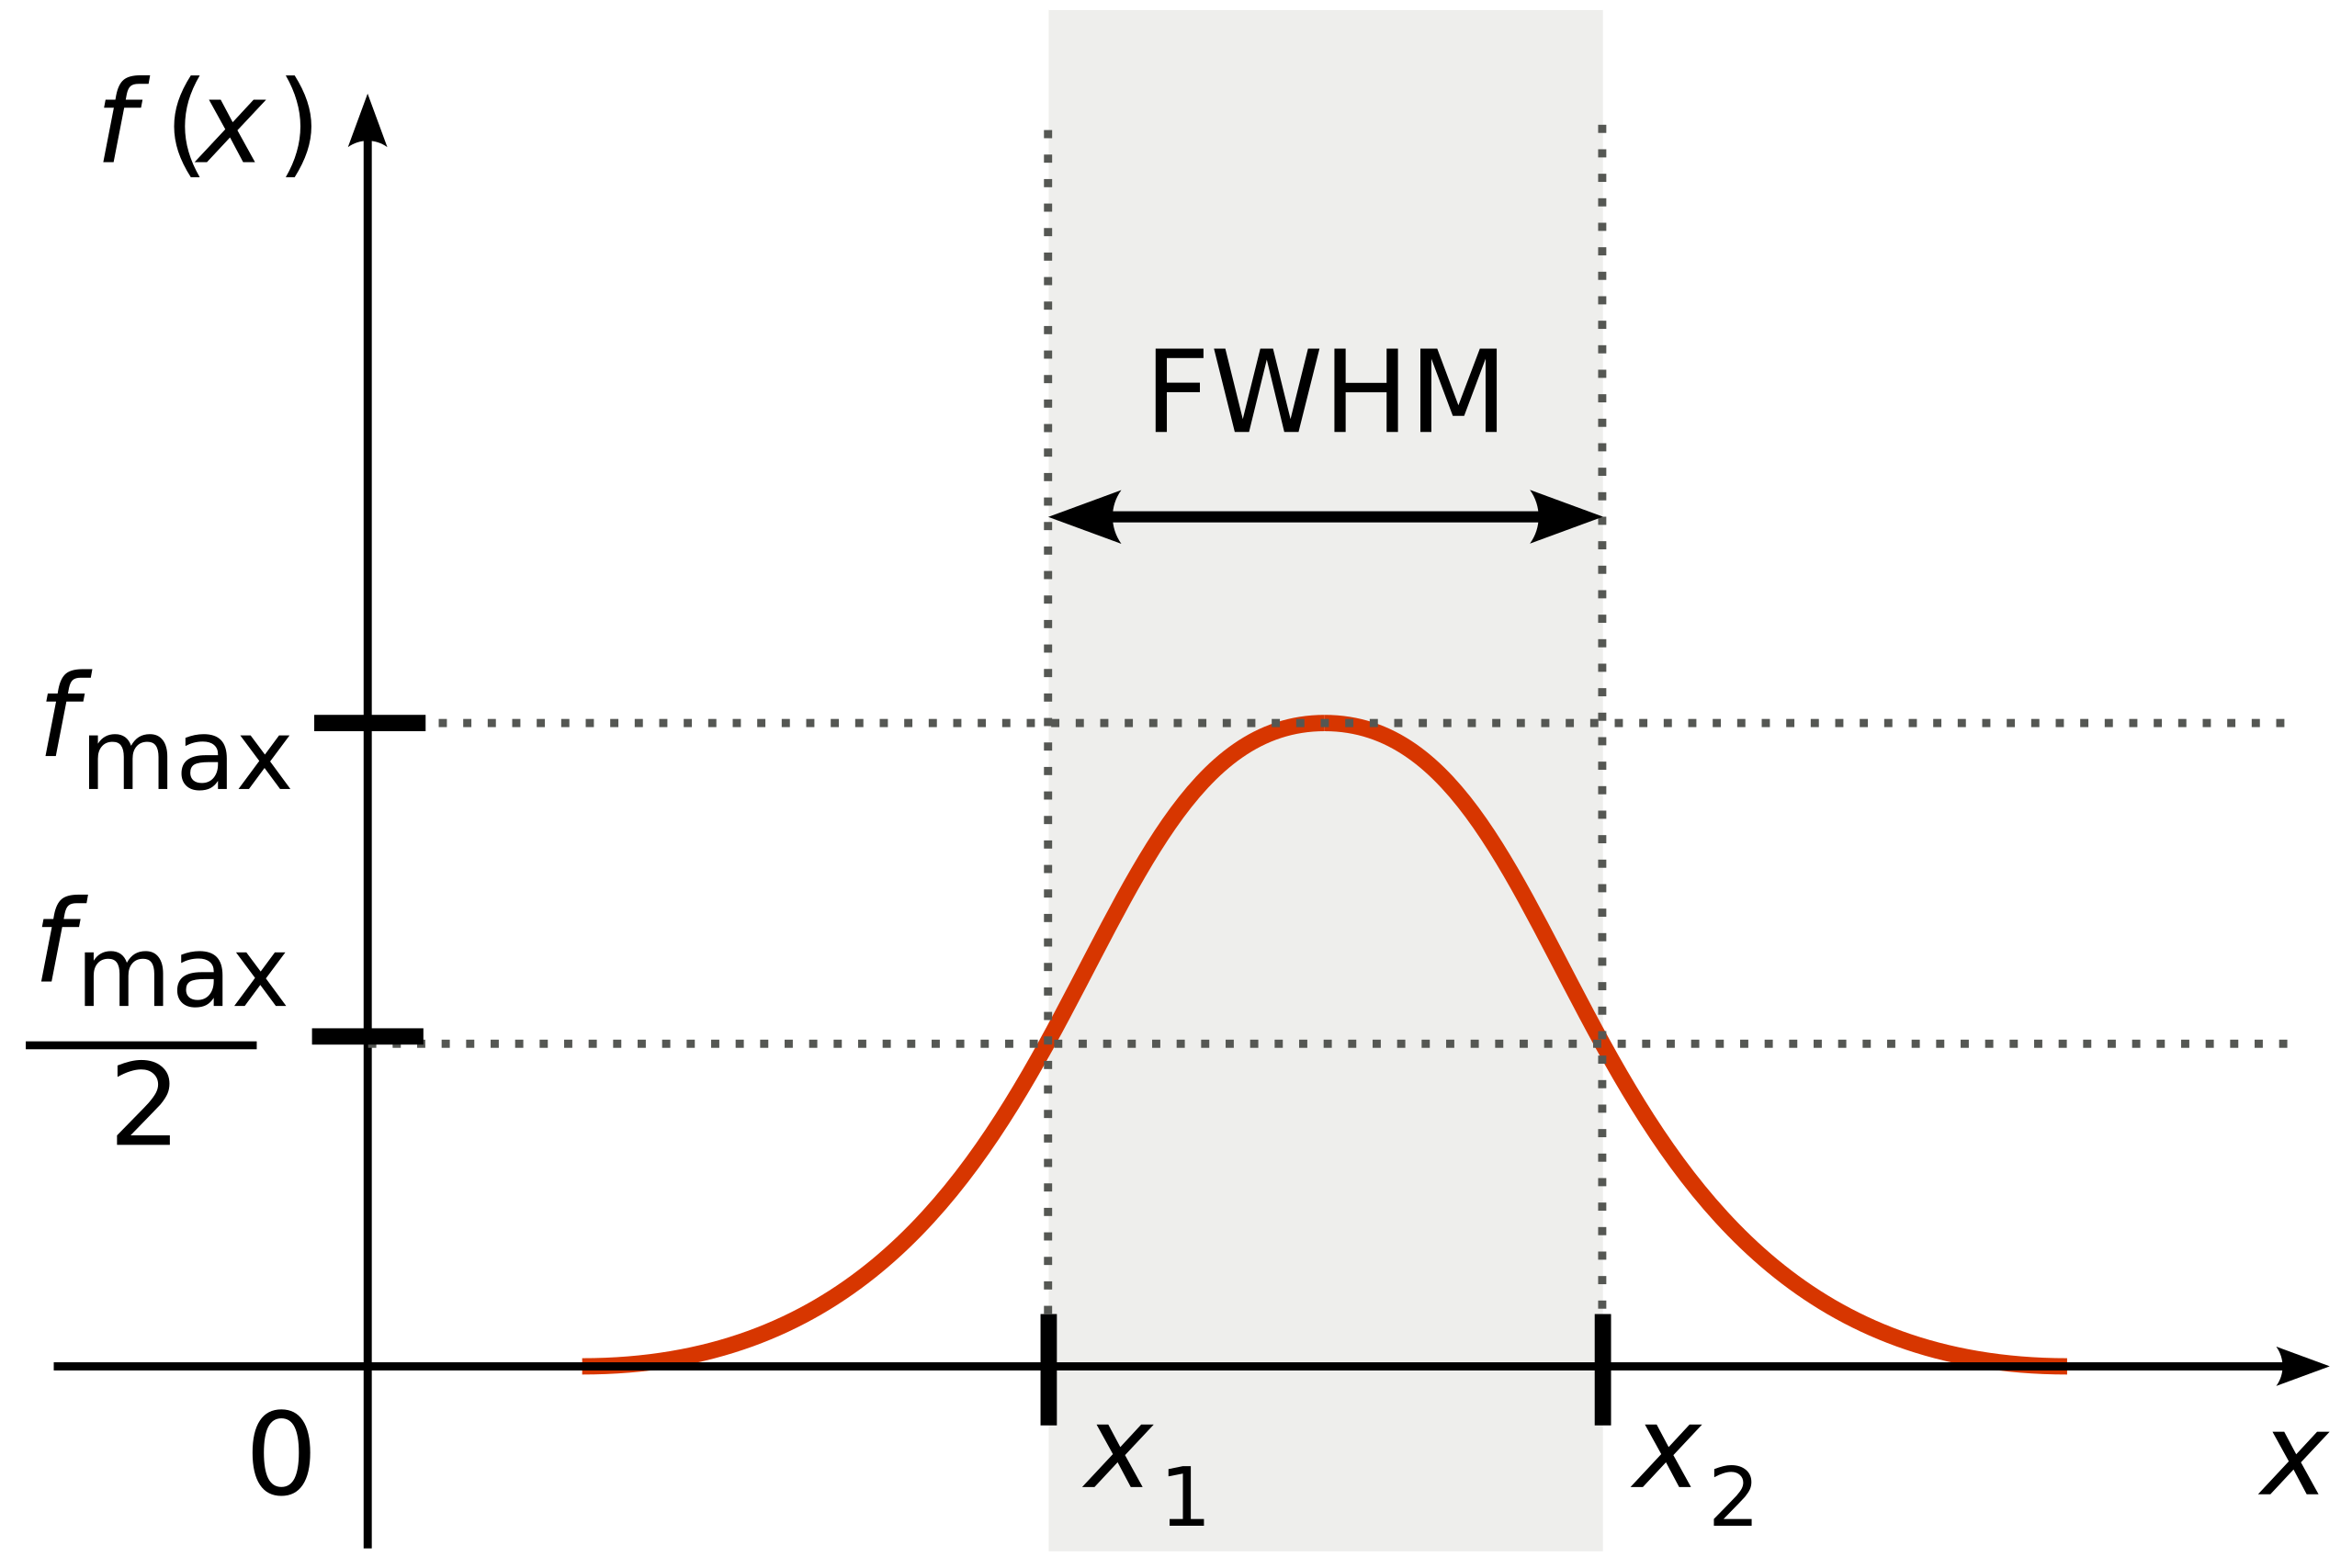
\includegraphics[width=0.5\textwidth]{assets/figures/théorie/FWHM.png}
  \caption[Illustration de la LMH]{Illustration de la largeur à mi-hauteur \autocite{largeur_mis_hauteur}\footnotemark}\label{fig:largeur_mis_hauteur}
\end{figure}

\footnotetext{\fullcite{largeur_mis_hauteur}}
Un seeing étant $\leq  0.4$" d'arc est considéré comme excellent, au DAG le seeing est usuellement de 0.9".

Une autre façon de quantifier le seeing est le paramètre de Fried $\mathbf{r_0}$. Pour expliquer le paramètre $r_0$, c'est le diamètre en cm qu'aurait un télescope
qui fournirait, en l'absence de turbulences, la même image que notre télescope en présence de turbulences. C'est ce paramètre $r_0$ qui sera utilisé en suite pour caractériser les écrans de phase.

La formule qui sera utilisée dans le calcul du paramètre de Fried sera :
\begin{equation}
  \sigma_{a_j}^2 \sim F(j) \cdot (\frac{D}{r_0})^{5/3} \label{eq:param_fried}
\end{equation}

Où :
\begin{itemize}
  \item $\sigma_{a_j}^2$ = la variance des coefficients de Zernike j
  \item  $F(j)$ = variance des coefficients de Zernike pour D/r0 = 1
  \item $D$ = diamètre du téléscope
  \item $r_0$ = paramètre de Fried
\end{itemize}

\subsection{Les turbulences atmosphériques}

\subsubsection{Cause physique}
L'atmosphère de notre planète n'est pas un bloc homogène, cette dernière est composée de \textbf{masses d'air}. Ces masses d'air
sont des zones de l'atmosphère où les conditions de température, de pression et d'humidité sont homogènes \cite{masse_air_wiki}\cite{masse_air_unige}.
L'écoulement de ces zones se fait en régime turbulent à des vitesses usuellement mesurées entre 1 et 20 m/s sur des longueurs de 10 à 1000m, ce phénomène
turbulent des mouvements de masses d'air sera qualifié de \textbf{turbulence dynamique} dans la suite de ce rapport.

Cette turbulence dynamique (la vitesse de l'écoulement) n'a pas d'incidence directe sur la propagation des ondes lumineuses, seul l'indice de réfraction de l'atmosphère influence la propagation
de la lumière. L'indice de réfraction est influencé par la densité de l'air selon la loi de Dale-Gladstone:

% \begin{equation}
%     N = 77.6 (\frac{P}{T}) + 3.74\cdot 10^5 (\frac{e}{T^2}) + C\frac{n_e}{f^2}
% \end{equation}

% Où:
% \begin{itemize}
%     \item $P$ = pression exprimée en hPa
%     \item $T$ = température absolue (K)
%     \item $e$ = pression de vapeur d'eau contenue dans l'air (hPa)
%     \item $C$ = $4,03 \cdot 10^{-7} m^{-3}Hz^2$
%     \item $n_e$ = densité électronique
%     \item $f$ = fréquence du signal
% \end{itemize}

\begin{equation}
  n-1 \sim \rho = \alpha_n \cdot \frac{P}{T}
\end{equation}

Où:
\begin{itemize}
  \item $P$ = pression exprimée en $N/m^2$
  \item $T$ = température absolue (K)
  \item $\alpha_a$ = $80\cdot10^{-8} K/Pa$
\end{itemize}

Pour aller plus loin, c'est généralement la température qui aura une grande influence sur l'indice de réfraction de l'air
et non la pression, car cette dernière est constante dans toute l'épaisseur d'une couche turbulente. Cette perturbation d'indice de
réfraction entre les couches turbulentes est donc la source des \textbf{Turbulences optiques}\cite{thèse_laurent_turbulence}.

\newpage
\subsubsection{Types de turbulences}
Plusieurs types de turbulences optiques sont observables à des altitudes bien spécifiques,
il est possible d'en distinguer 4 types :

\say{

  \begin{itemize}
    \item \textbf{1. Turbulence de coupole :}
          \newline
          Elle apparaît lorsque l'air n'a pas la même température à l'intérieur et à l'extérieur de la coupole (du télescope). Cette dernière
          correspond à la turbulence du miroir.

    \item \textbf{2. Turbulence de surface :}
          \newline
          Active sur les premiers 10 à 100m. Elle doit son origine au refroidissement par convection du sol chauffé par le rayonnement solaire.
          Typiquement, elle atteint un minimum juste après le lever du soleil, puis augmente régulièrement jusqu'au début de l'après-midi. Elle décroit
          ensuite pour atteindre un second minimum après le coucher du soleil, puis augmente légèrement durant la nuit. Le moyen de minimiser au maximum cette turbulence
          est le choix du site d'installation du télescope. Par exemple, placer le télescope en haut d'une tour loin de toute surface minimisera le phénomène.

    \item \textbf{3. Turbulence de moyenne altitude 1-5/6 Km :}
          \newline
          Elle trouve son origine à la fois dans les perturbations orographiques (ondes générées par les reliefs) des courants atmosphériques et dans les instabilités thermiques
          de l'atmosphère. Elle est constituée par une multitude de fines couches turbulentes de quelques centaines de mètres d'épaisseur. Ici encore, seule la sélection du site d'accueil est susceptible
          de minimiser cette composante.

    \item \textbf{4. Turbulence de tropopause et stratosphérique :}
          \newline
          Au-delà de $\approx 6 $Km, on observe une certaine systématique pour la plupart des sites :
          la turbulence atteint un minimum entre 6 et 10 Km, puis augmente à nouveau pour atteindre un maximum dans la tropopause (zone de transition entre la troposphère et la stratosphère), 10-20 Km. Cette couche
          turbulente est due à la présence de forts vents cisaillant l'atmosphère, très fréquents à la limite de la troposphère. La turbulence optique diminue en suite dans la stratosphère, pour finalement disparaître
          au-delà de 25 à 30 Km d'altitude.
  \end{itemize}

} \footnotemark


\footnotetext{\cite{thèse_laurent_turbulence_types}\fullcite{thèse_laurent_turbulence_types}}

\newpage
\subsubsection{Illustration des effets des turbulences}

Pour illustrer concrètement les effets des turbulences, ainsi que donner une idée de l'impact de la valeur du seeing sur la PSF\footnotemark (Point Spead Function) d'un télescope
:
\begin{figure}[H]
  \centering
  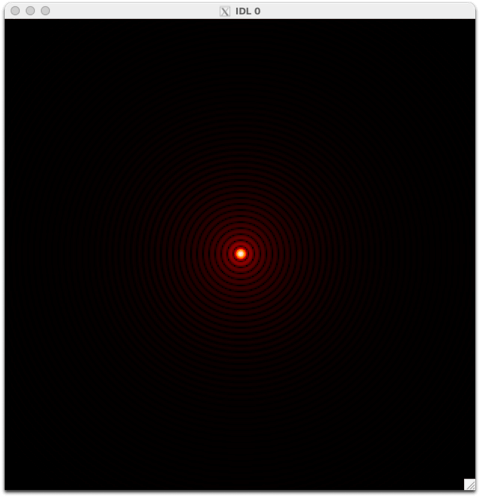
\includegraphics[width=0.5\textwidth]{assets/figures/théorie/PSF_parfaite.png}
  \caption[PSF parfaite]{PSF parfaite d\textquotesingle un télescope de 1m de diamètre, longueur d'onde 500 nm}
\end{figure}

\begin{figure}[H]
  \centering
  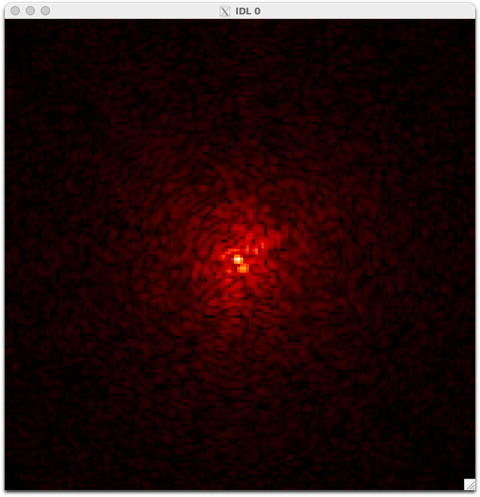
\includegraphics[width=0.5\textwidth]{assets/figures/théorie/PSF_seeing_1second.png}
  \caption[PSF avec seeing 1"]{PSF du même télescope, avec image instantanée pour un seeing de 1"}
\end{figure}
\footnotetext{La PSF décrit la distribution d\textquotesingle intensité de la lumière provenant d\textquotesingle un point source.}
\begin{figure}[H]
  \centering
  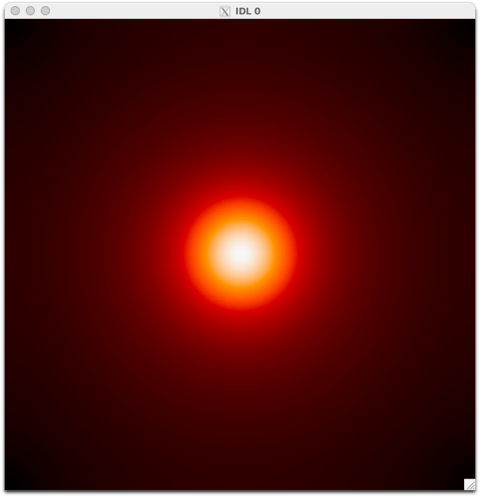
\includegraphics[width=0.5\textwidth]{assets/figures/théorie/PSF_turbulente.png}
  \caption[PSF turbulente]{PSF turbulente, longue exposition}
\end{figure}

Il est donc possible d'observer l'impact de la turbulence sur une image instantanée et sur une image à longue exposition, cela résultera en une perte de détails et donc à une image
finale beaucoup plus douce.


\subsection{Front d'onde et coefficients de Zernike}
\subsubsection{Front d'onde}
Un front d'onde est une surface imaginaire qui relie tous les points d'une onde ayant la même phase à un instant donné.
Pour la lumière, cela signifie que tous les points sur un front d'onde ont parcouru la même distance depuis la source lumineuse et oscillent en phase.
Le front d'onde est perpendiculaire à la direction de la lumière, donc une réfraction modifiera de manière prédictible le front d'onde :

\begin{figure}[H]
  \centering
  \begin{subfigure}{.5\textwidth}
    \centering
    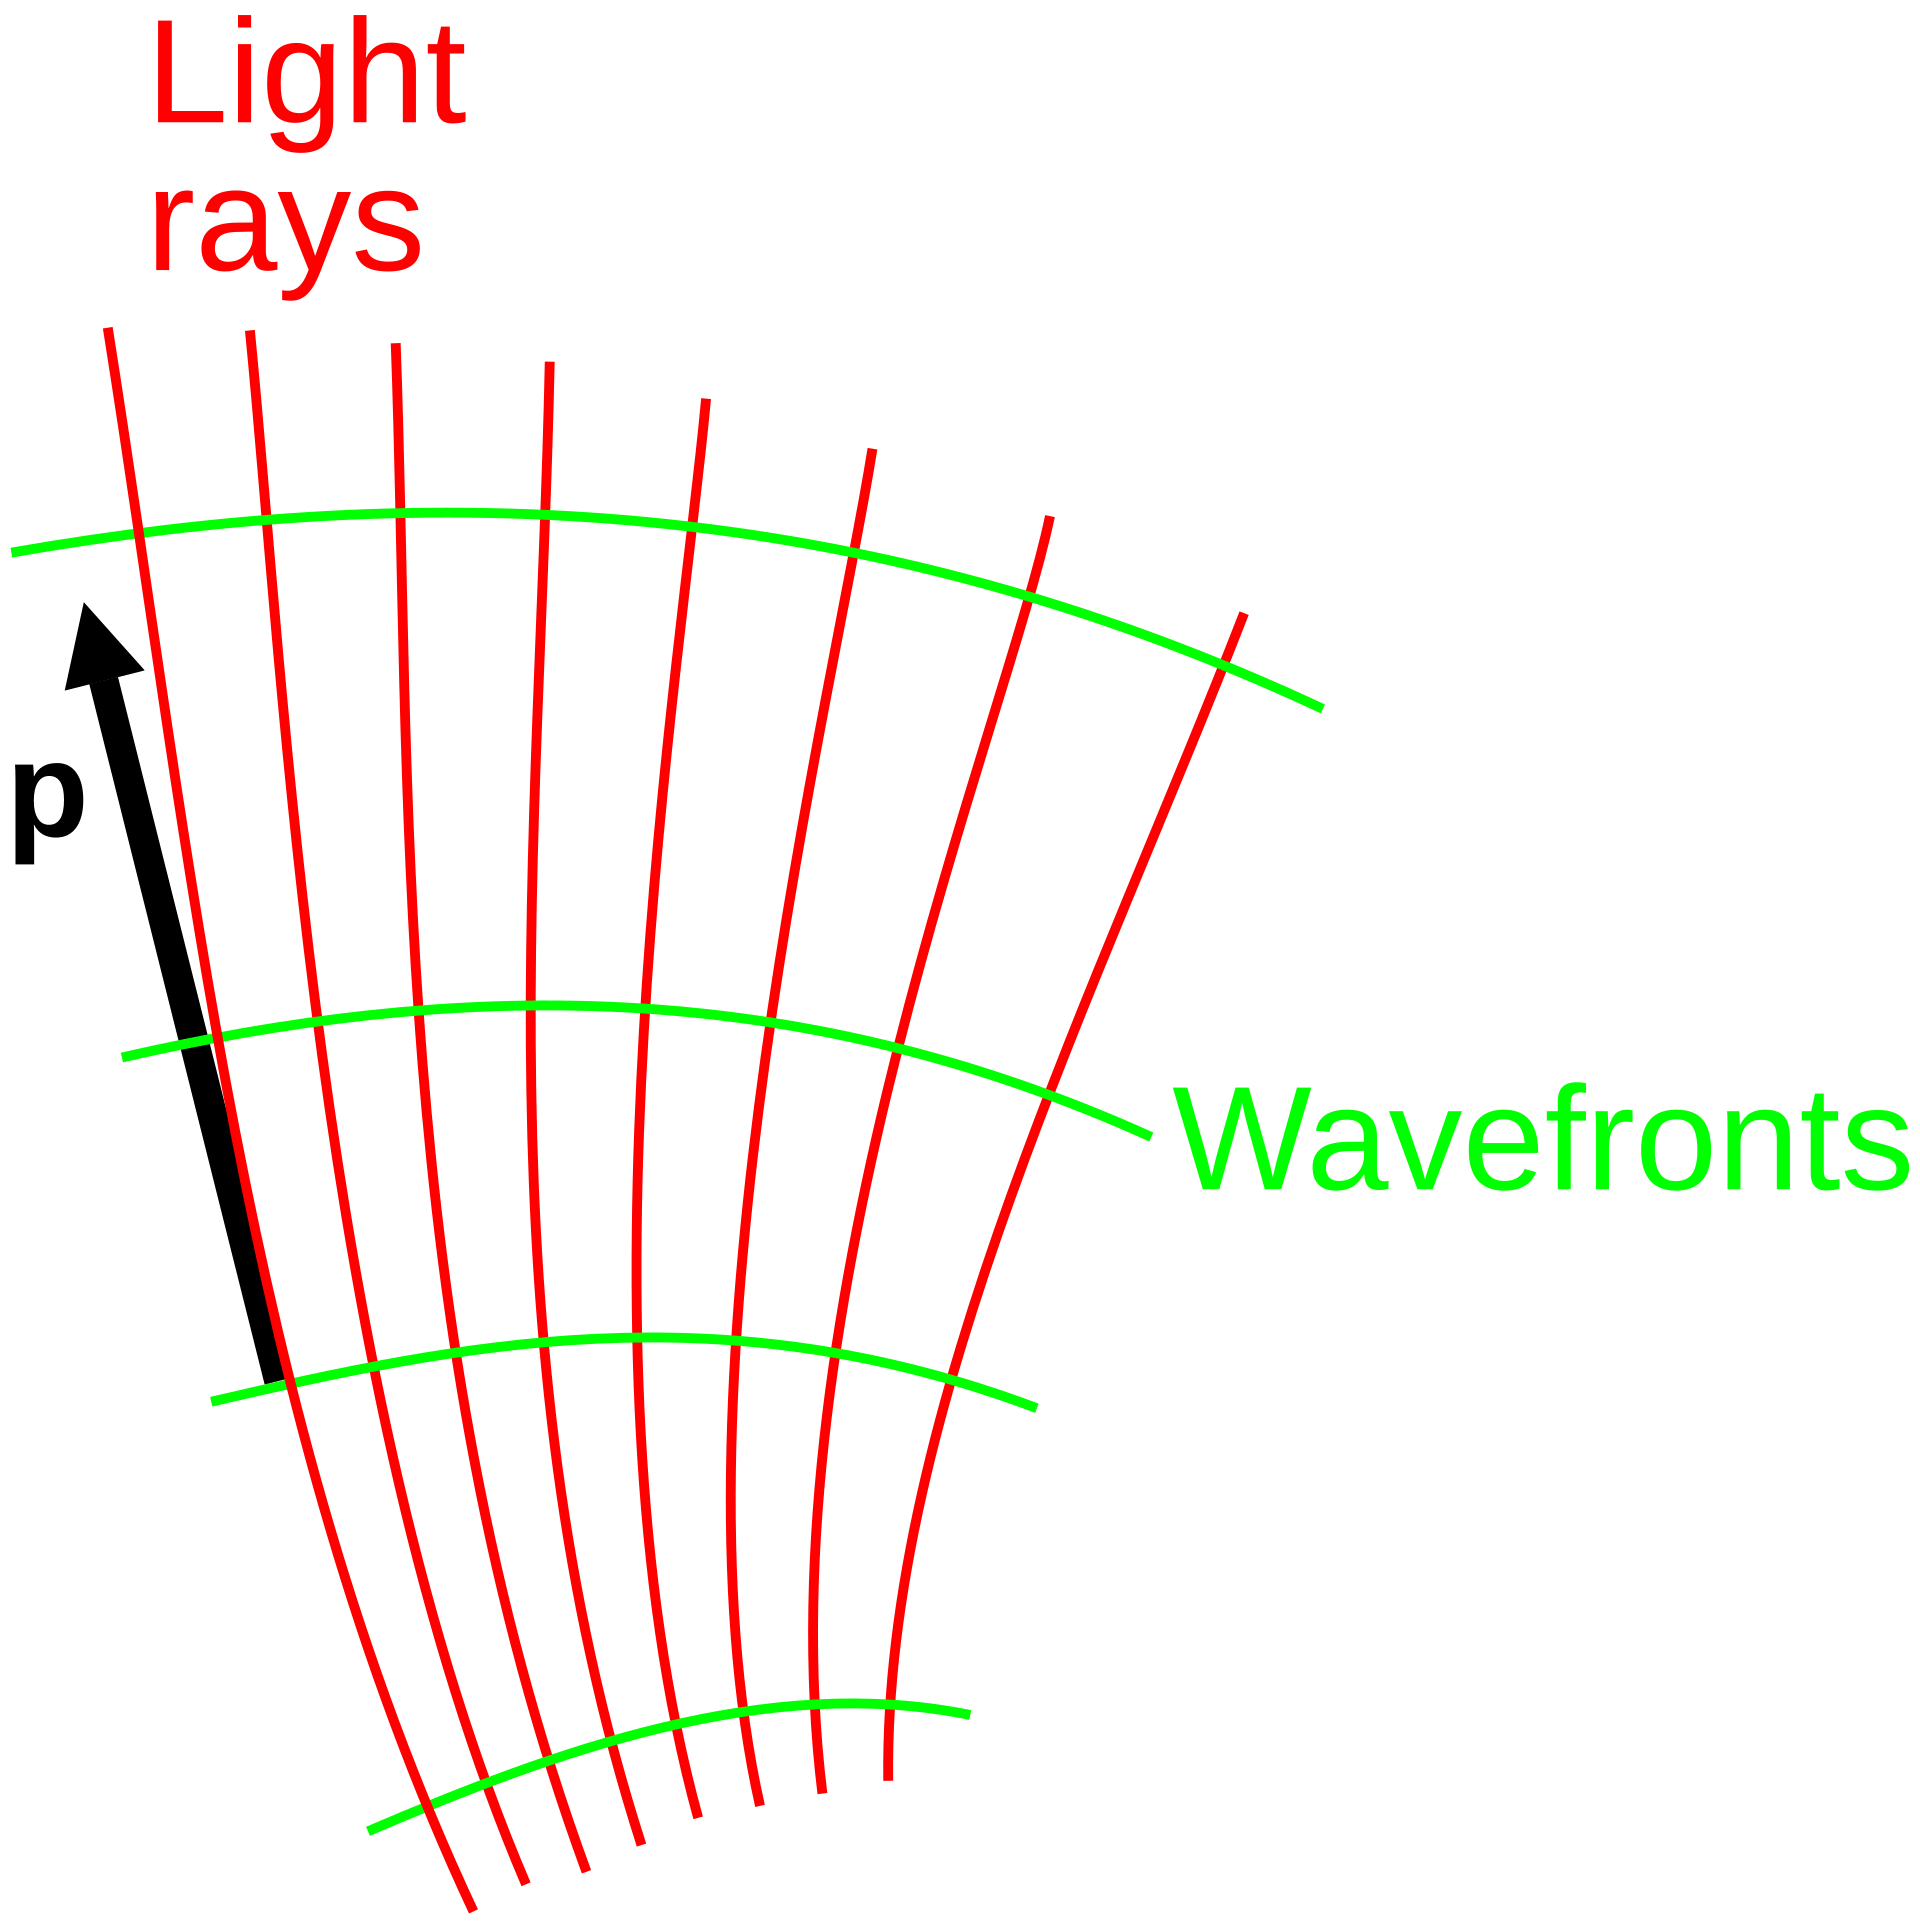
\includegraphics[width=.75\linewidth]{assets/figures/théorie/wavefront_representation.png}
    \caption{Représentation du front d'onde perpendiculaire}
    \label{fig:front_onde_perp}
  \end{subfigure}%
  \begin{subfigure}{.5\textwidth}
    \centering
    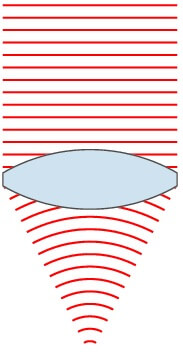
\includegraphics[width=.4\linewidth]{assets/figures/théorie/Lens_and_wavefronts.jpeg}
    \caption{Modification du front d'onde après réfraction}
    \label{fig:refraction_front_onde}
  \end{subfigure}
  \caption[Illustration front d'onde]{Illustrations du principe de front d'onde \cite{wavefront_wikipedia}\footnotemark}
  \label{fig:illu_front_onde}
\end{figure}
\footnotetext{\fullcite{wavefront_wikipedia}}

\subsubsection{Mesure du front d'onde}

Pour mesurer le front d'onde, on emploie un \textbf{capteur de front d'onde Shack-Hartmann} du fabricant Thorlabs:

\begin{figure}[H]
  \centering
  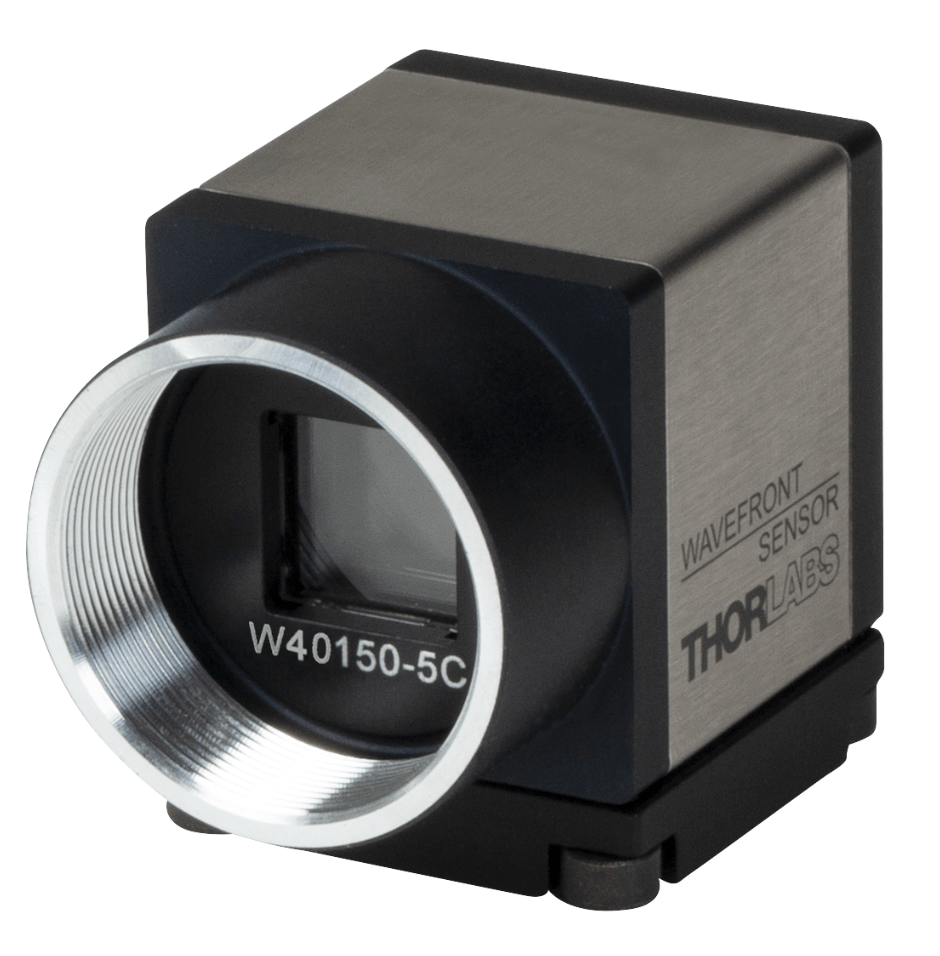
\includegraphics[width = 0.4\textwidth]{assets/figures/théorie/WFS40_7AR.png}
  \caption[Fonctionnement WFS Thorlabs]{Fonctionnement du capteur de front d'onde\cite{WFS_thorlabs_site}\footnotemark}
  \label{fig:WFS_thorlabs_fonctionnement}
\end{figure}
\footnotetext{\fullcite{WFS_thorlabs_site}}


Le principe de fonctionnement d'un capteur de Shack-Hartmann est le suivant :

\begin{figure}[H]
  \centering
  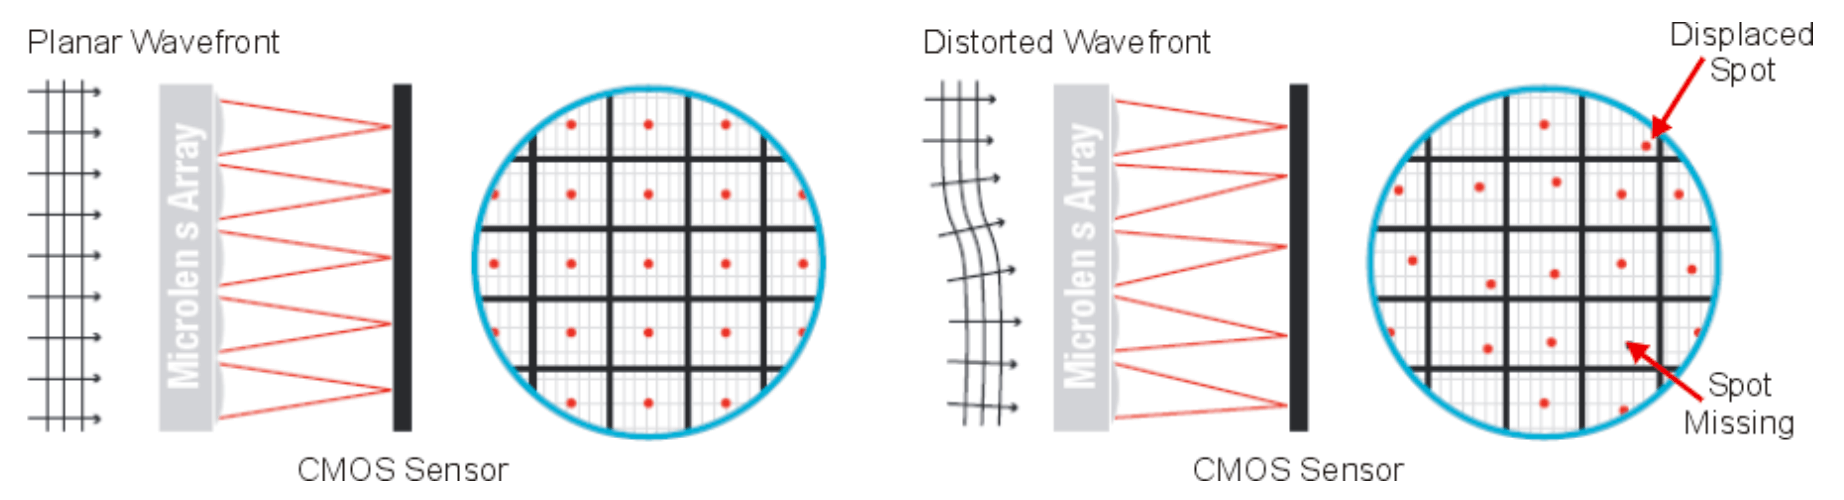
\includegraphics[width = 1.1\textwidth]{assets/figures/théorie/Shack_Hartmann_Wavefront_Distorted.png}
  \caption[Image WFS Thorlabs]{WFS4\_7AR de Thorlabs\cite{WFS_thorlabs_site}\footnotemark}
  \label{fig:WFS_thorlabs}
\end{figure}
\footnotetext{\fullcite{WFS_thorlabs_site}}

\say{ Un capteur de Shack-Hartmann consiste en une grille de lentilles et une caméra. Quand un front d'onde entre dans la matrice de lentilles,
  un champ de points est créé sur la caméra. La position de chaque point est analysée pour mesurer dynamiquement le front d'onde
  de sources laser ou pour caractériser la distorsion de front d'onde causée par des composants optiques. }\footnotemark[5]

Ce capteur nous est donc utile, car ce dernier permet de mesurer et de représenter le front d'onde du du faisceau lumineux passant à travers la turbulence
optique, ou alors, dans notre cas, à travers l'écran de phase, il retourne aussi les coefficients de Zernike du front d'onde.

\newpage
\subsubsection{Coefficients de Zernike}

Les coefficients de Zernike sont les "poids" polynômes de Zernike, c'est-à-dire la contribution que chaque polynome a pour décrire les aberrations de front d'onde,
ces derniers permettent de décrire n'importe quelle surface dans un domaine circulaire.
\begin{figure}[H]
  \centering
  \begin{subfigure}{.5\textwidth}
    \centering
    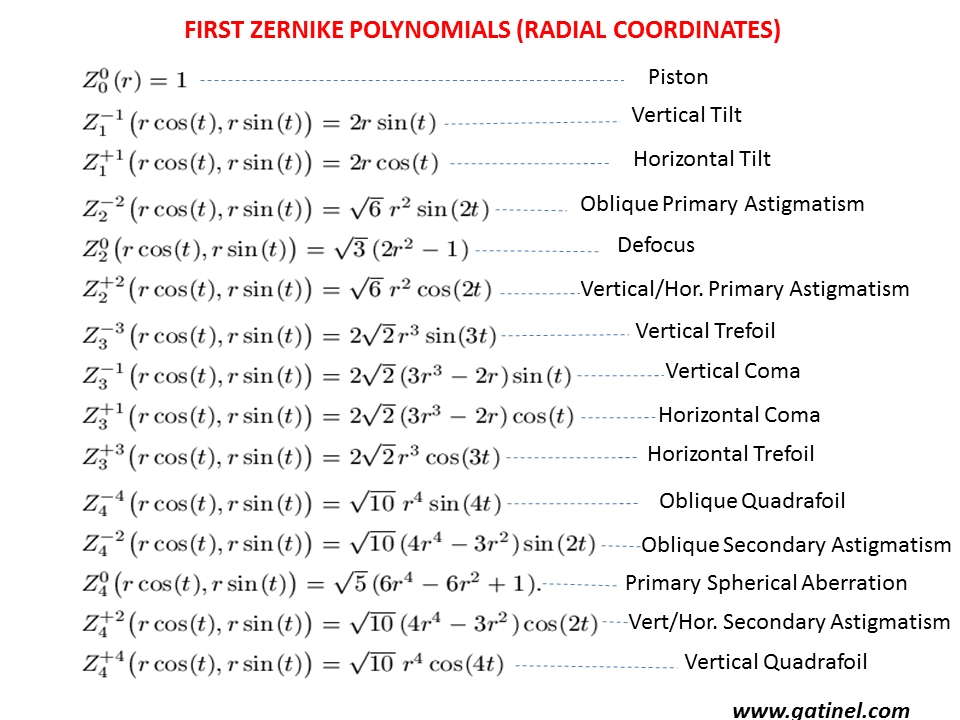
\includegraphics[width=1\linewidth]{assets/figures/théorie/Zernike-polynomials-equations.png}
    \caption{Formules des polynômes de Zernike}
    \label{fig:formules_poly_Zernike}
  \end{subfigure}%
  \begin{subfigure}{.5\textwidth}
    \centering
    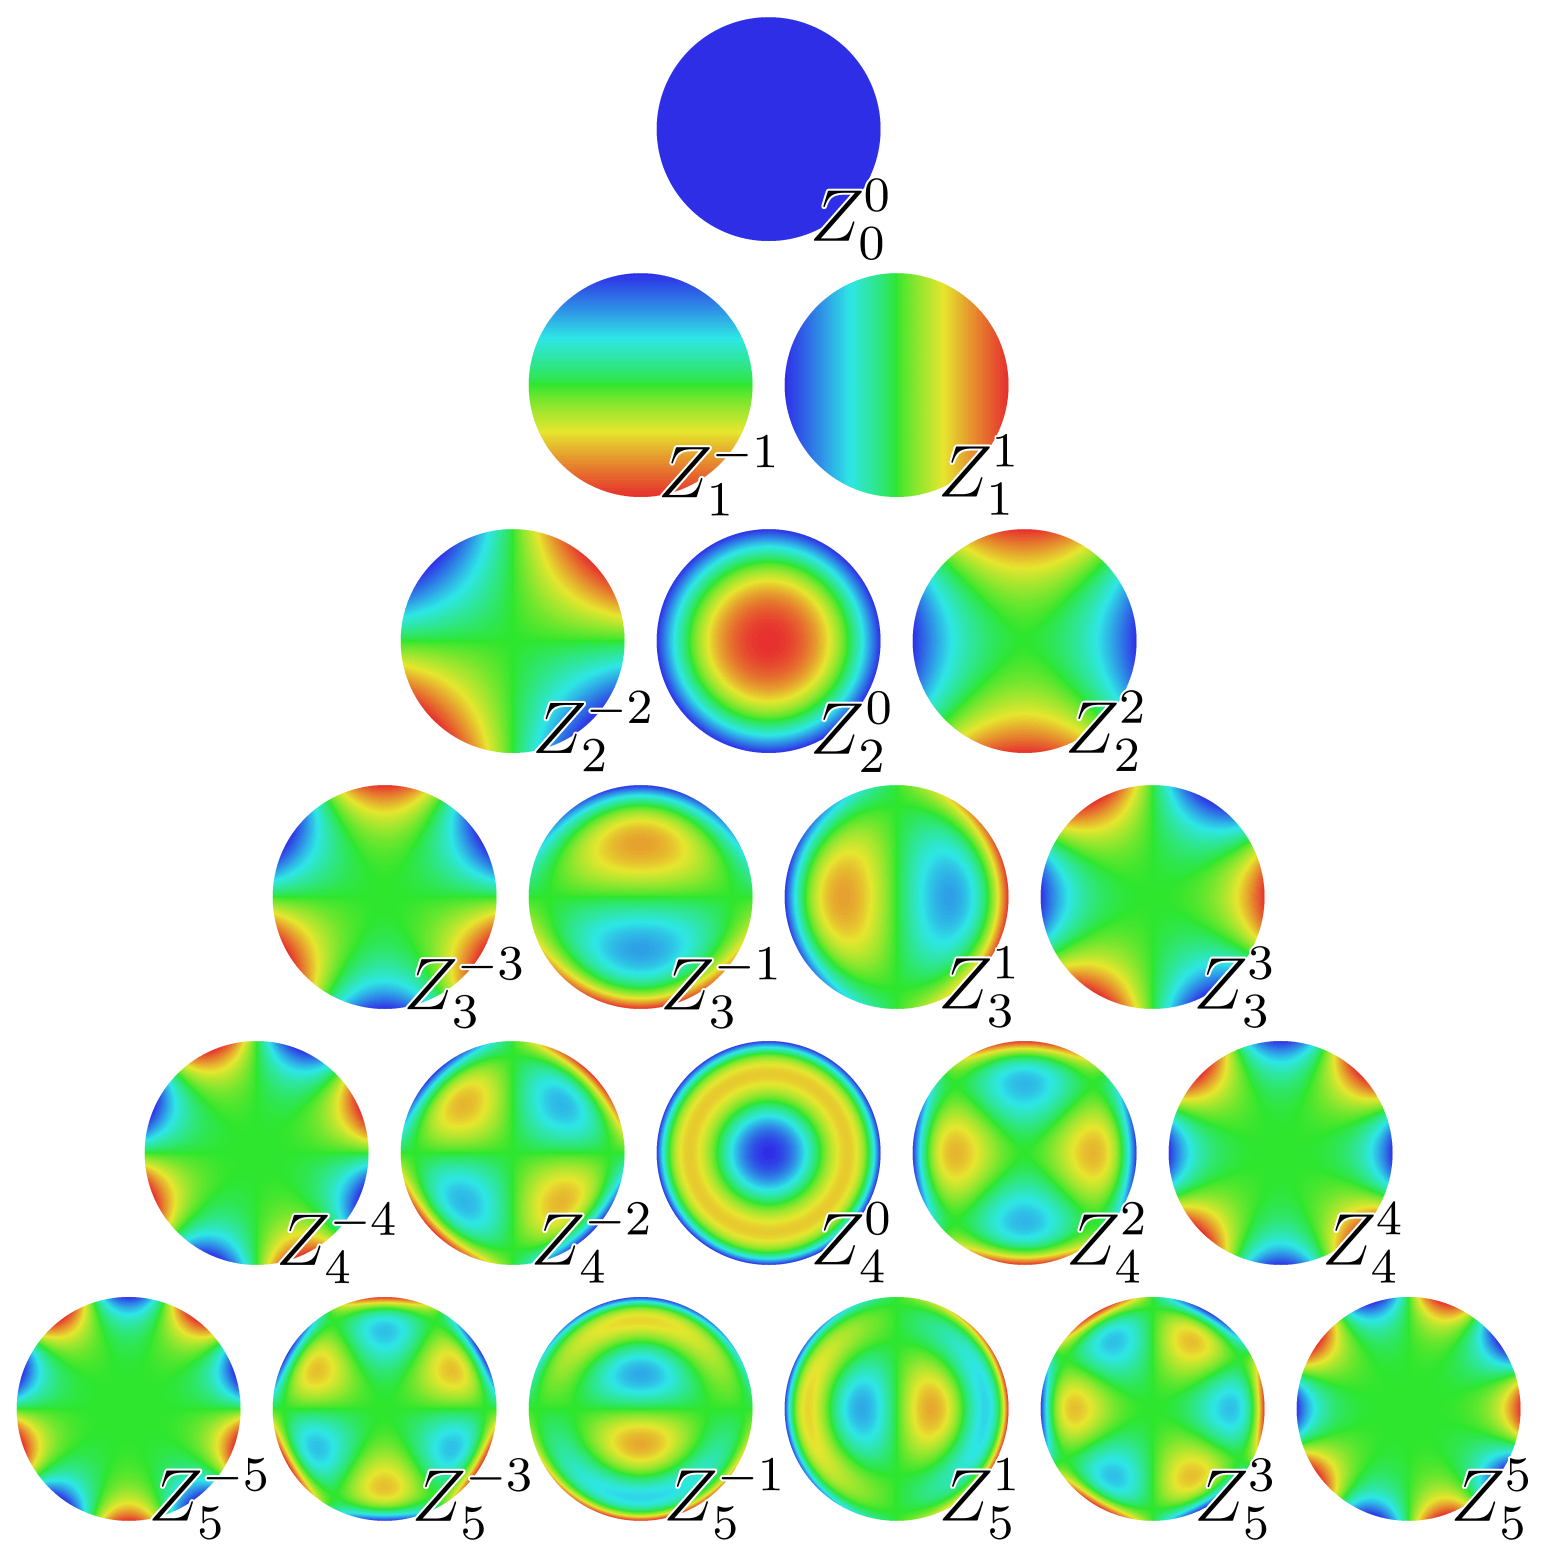
\includegraphics[width=.75\linewidth]{assets/figures/théorie/zernike_polynomes_plots.png}
    \caption{Représentation des polynômes de Zernike}
    \label{fig:plots_des_polynomes_Zernike}
  \end{subfigure}
  \caption[Illustration polynômes de Zernike]{Illustration polynômes de Zernike \cite{Zernike_docteur_Damien}\footnotemark}
  \label{fig:illu_poly_Zernike}
\end{figure}

\footnotetext{\fullcite{Zernike_docteur_Damien}}

Pour reconstruire le front d'onde il suffit alors de sommer les fronts d'ondes des coefficients de Zernike. Autrement dit en équation cela donne :
\begin{equation}
  Front d'onde = \sum_{j=1}^{N}a_j * Z_j
\end{equation}

\chapter{Situation initiale}
Voici ci-dessous, la structure originale de la machine au commencement de ce projet de Bachelor :
\begin{figure}[H]
  \centering
  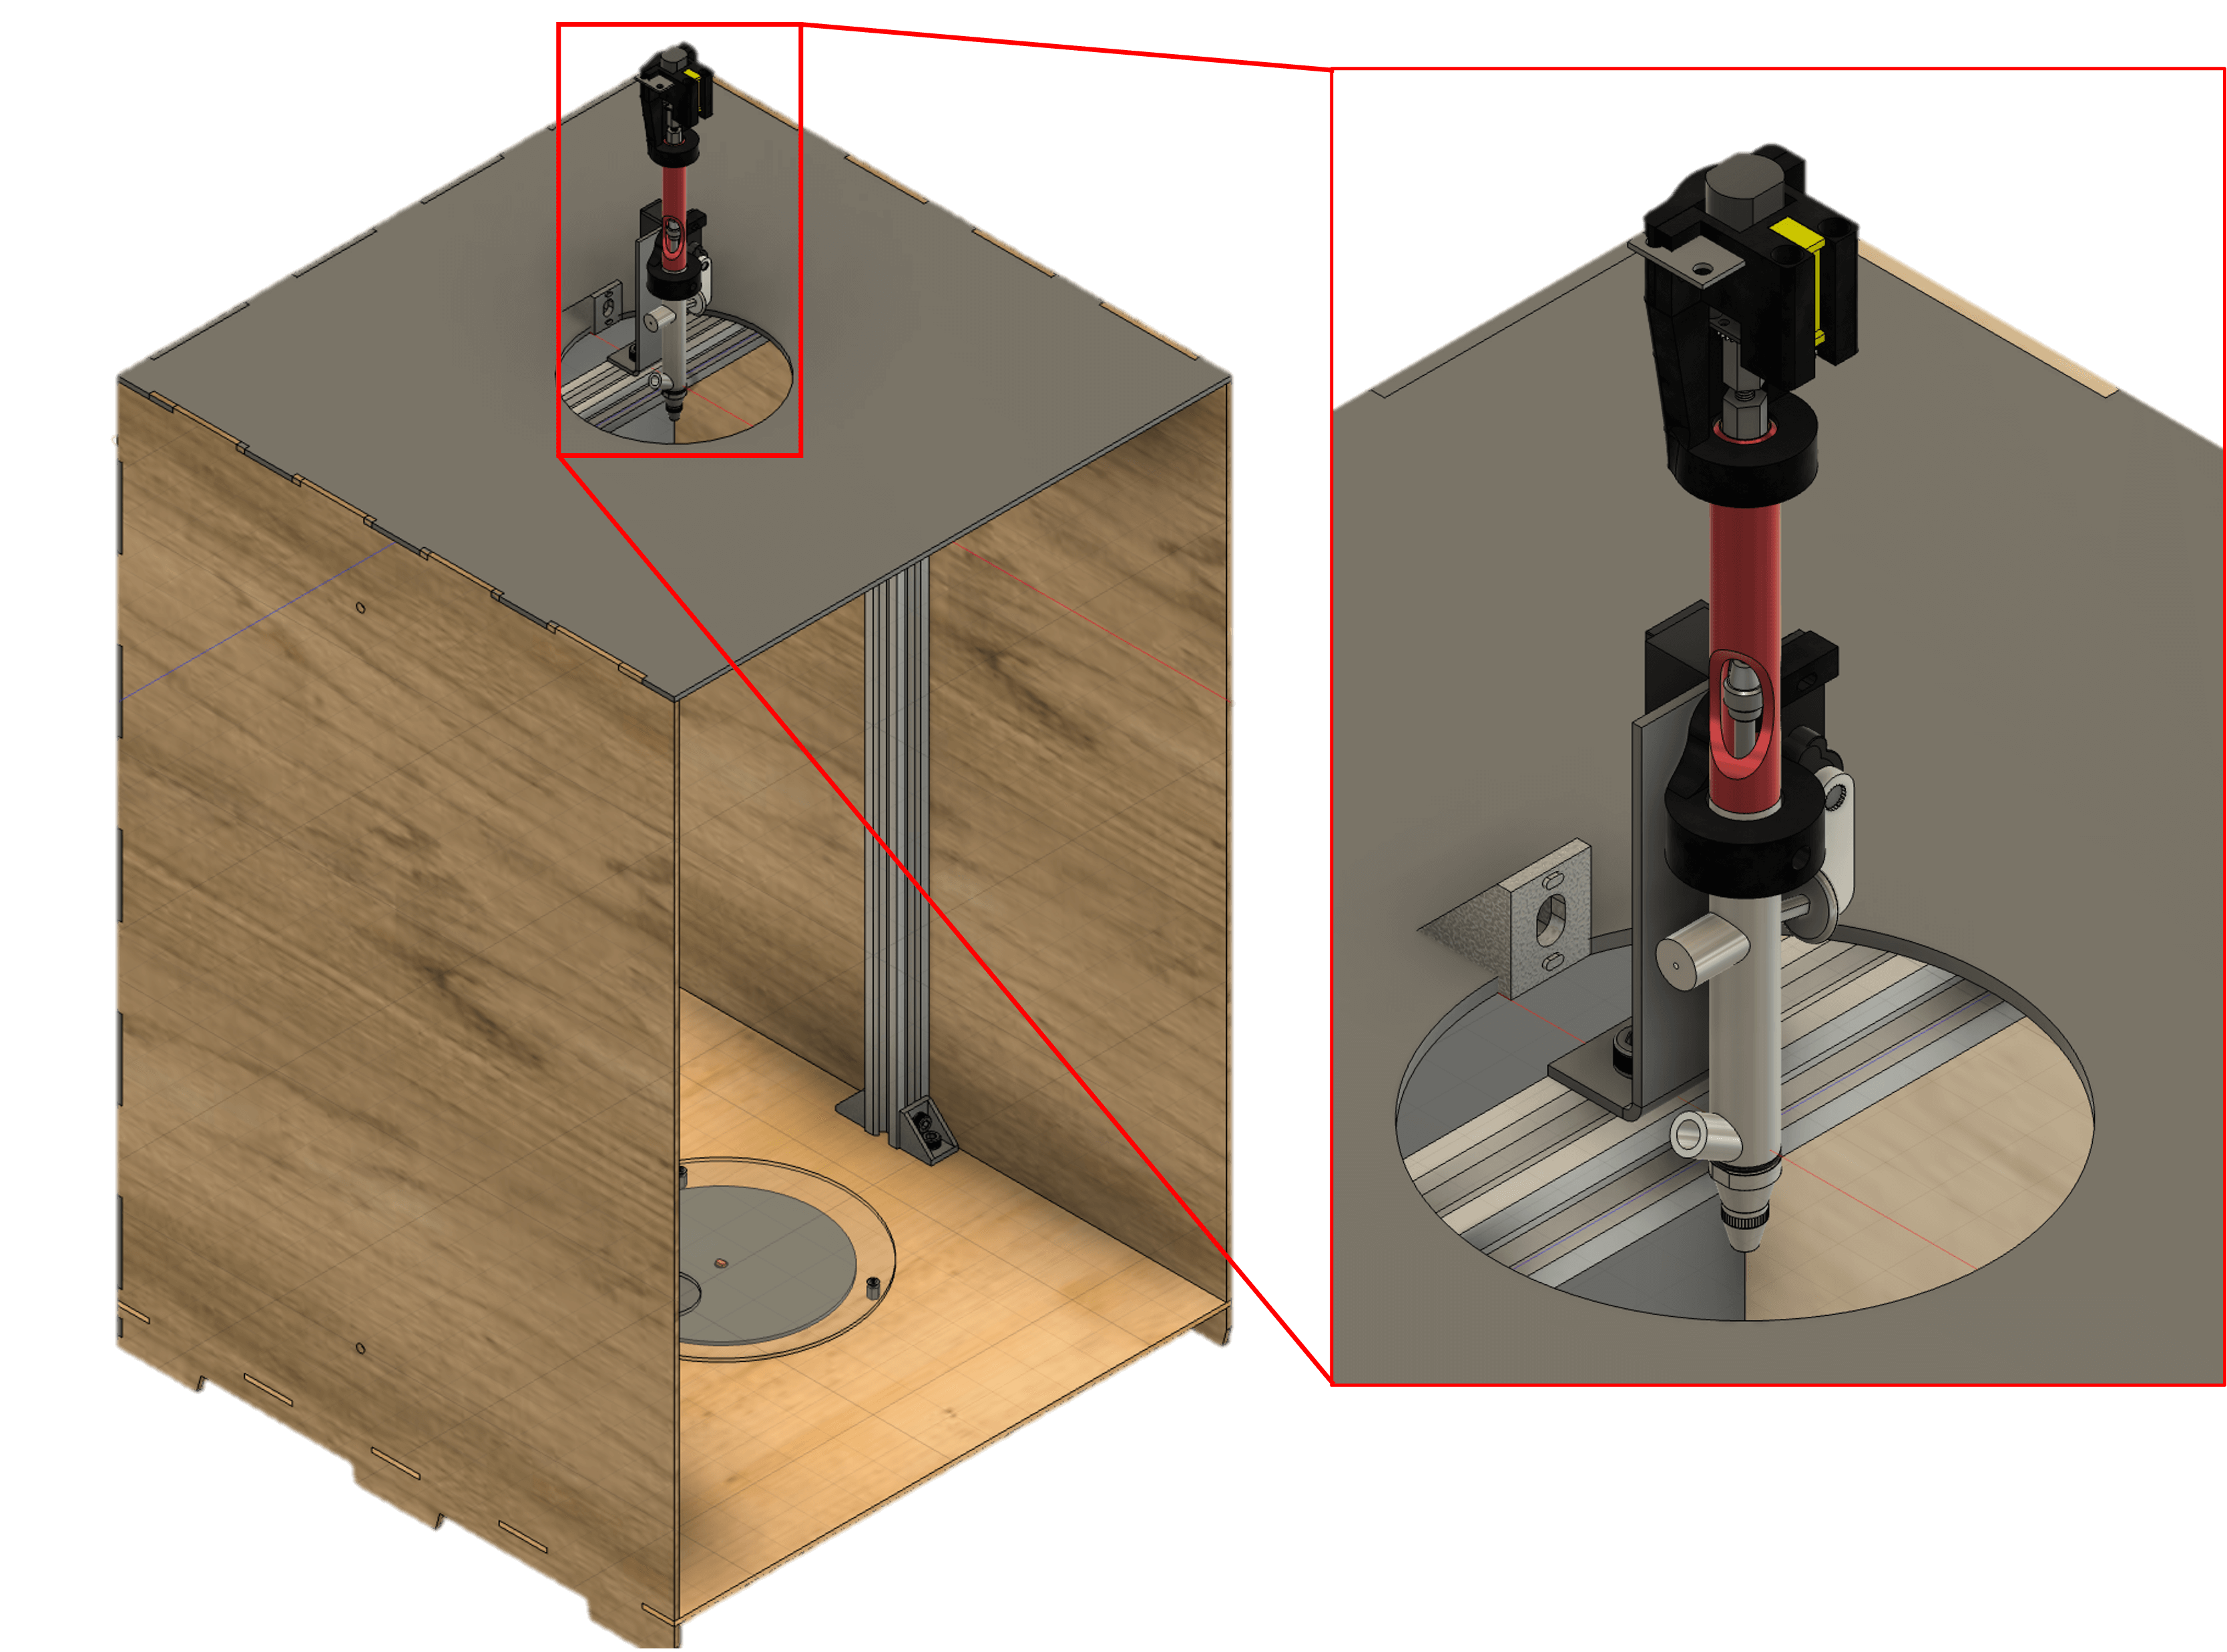
\includegraphics[width = \textwidth]{assets/figures/situation_initiale/machine_initiale.png}
  \caption[Machine originelle]{Machine originelle, avec un zoom sur le système de projection}
  \label{fig:Machine_originale}
\end{figure}

\newpage
La machine de projection se basait sur un aérographe robotisé, où des moteurs géraient les parties mobiles
de l'aérographe qui seraient normalement actionnée à la main :
\begin{figure}[H]
  \centering
  \begin{subfigure}{.35\textwidth}
    \centering
    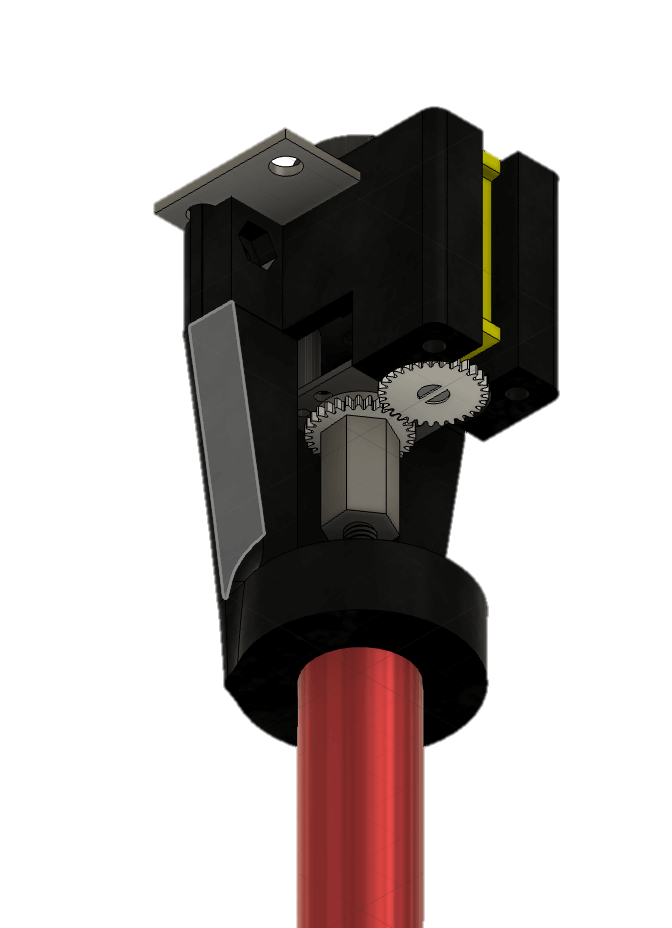
\includegraphics[width=1\linewidth]{assets/figures/situation_initiale/robotisation_aiguille.png}
    \caption{Robotisation de la position de l'aiguille}
    \label{fig:robot_aiguille}
  \end{subfigure}%
  \begin{subfigure}{.65\textwidth}
    \centering
    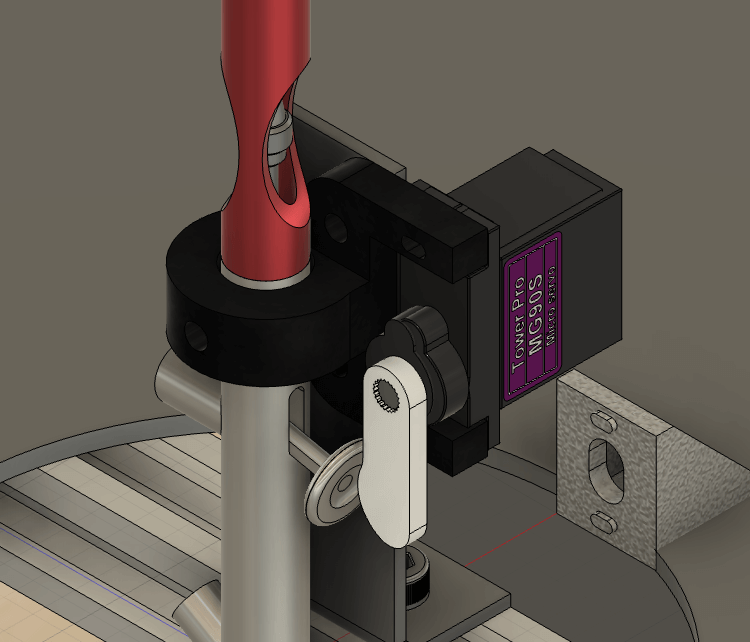
\includegraphics[width=.75\linewidth]{assets/figures/situation_initiale/Robotisation_projection.png}
    \caption{Robotisation du button d'activation du spray}
    \label{fig:robot_spray}
  \end{subfigure}
  \caption{Différentes robotisations de la machine originale}
  \label{fig:robotisations_aerographe}
\end{figure}

Un moteur pas-à-pas de type \textbf{28byj-48}, est situé en bas de l'appareil, ce dernier sert à faire tourner l'écran sur lui même,
c'est donc aussi où l'écran sera disposé lors de sa fabrication:
\begin{figure}[H]
  \centering
  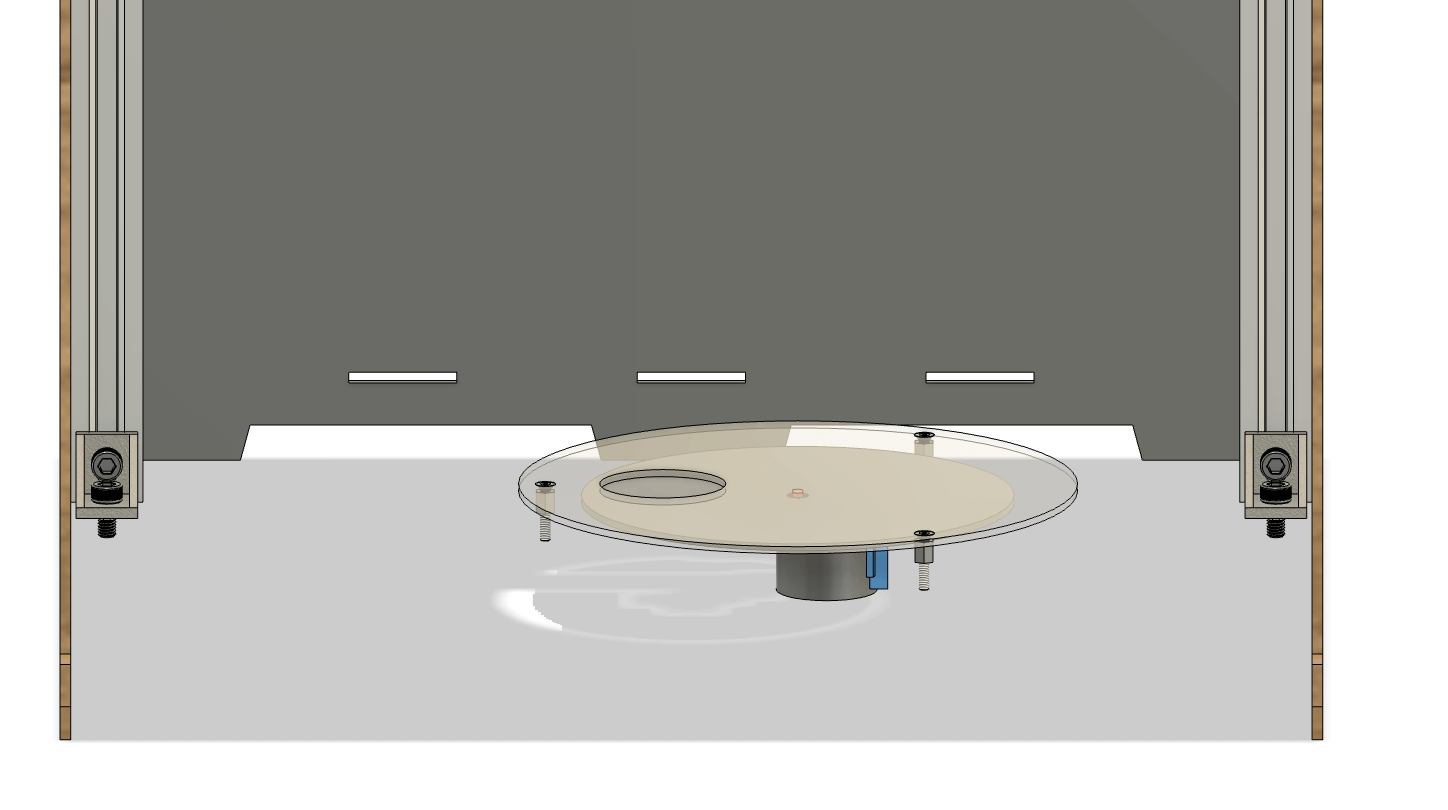
\includegraphics[width = \textwidth]{assets/figures/situation_initiale/rotation_ecran_initiale.png}
  \caption[Rotation écran initiale]{Système de rotation de l'écran}

\end{figure}

\newpage
Tout ces éléments sont contrôlés par un PCB et un arduino nano :
\begin{figure}[H]
  \centering
  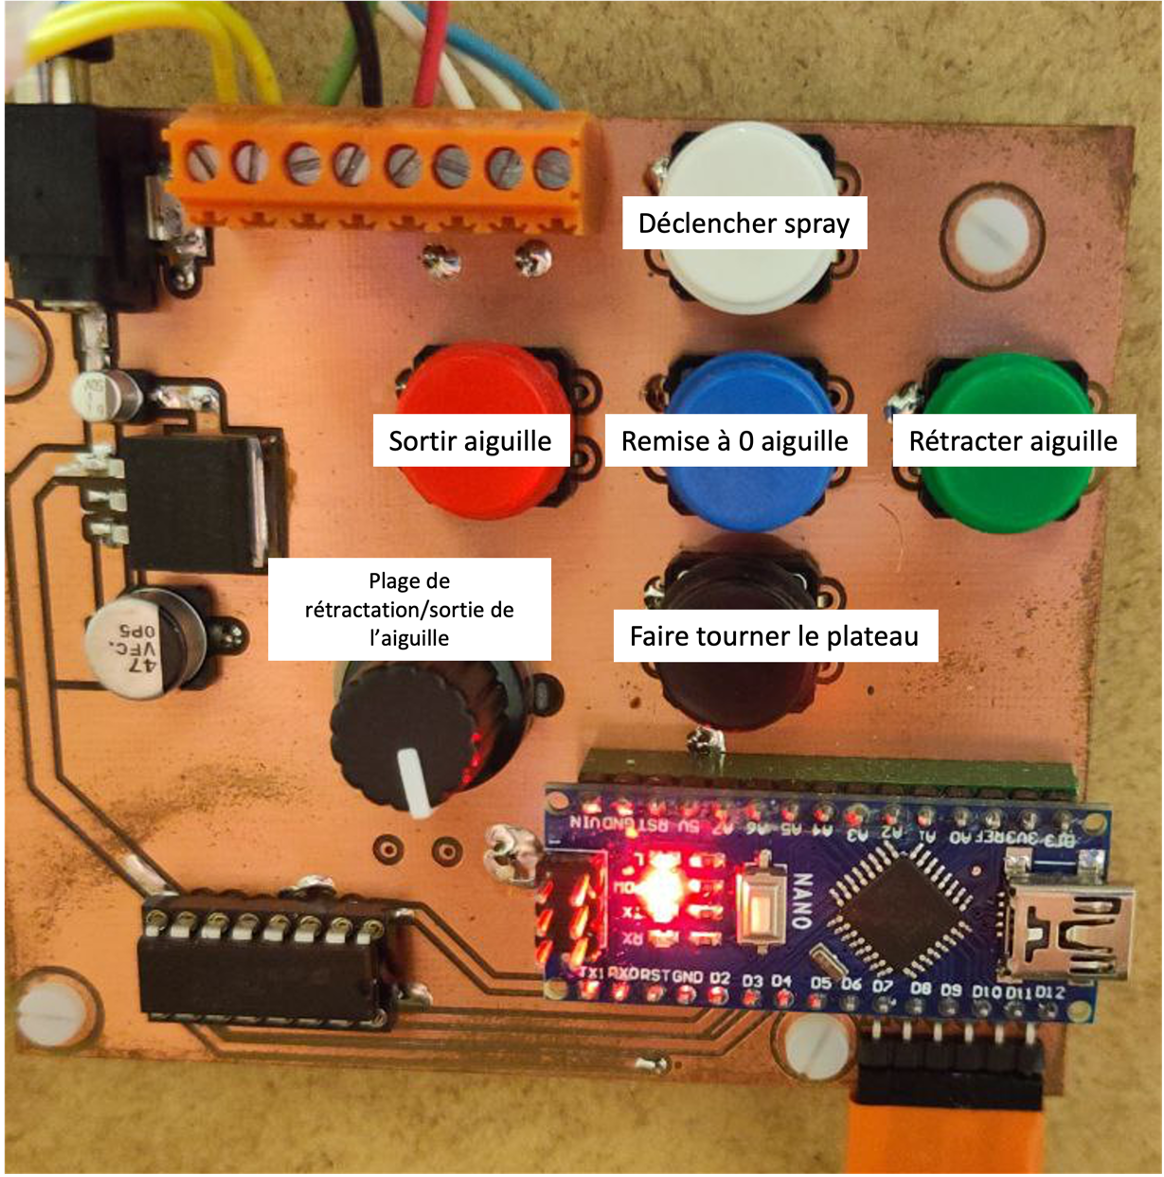
\includegraphics[width = 0.8\textwidth]{assets/figures/situation_initiale/PCB_machine_originale.png}
  \caption[PCB machine initiale]{PCB de la machine initiale et légende de chaque boutons}\label{PCB_machine_initial}
\end{figure}

\section{Problèmes avec la machine}
En effet, la machine d'origine présente plusieurs inconvénients.
\subsection{Aérographe}

\chapter{État de l'art}


%\section{État de l'art}
\section{Méthodes de projection de liquides}\label{sec:etat de lart}
\subsection{Bombe spray}
Pour constituer des écrans de turbulence aisément, l'approche de la bombe de spray pour les cheveux, ou de laque transparente pour surfaces a été employée.
\begin{figure}[H]
    \centering
    
\includegraphics[width=0.3\textwidth,trim={4cm 0 4cm 0},clip]{assets/figures/etat_art/airspray.jpeg}

    \caption{Bombe de laque (IA)}
\end{figure}
Cette solution étant assez sommaire et peu reproductible, elle a été abandonnée au profit de méthodes plus contrôlables.
La durée du "pschit" est sujette à l'erreur humaine, la quantité de liquide projetée
dépend directement de la durée d'appui, mais aussi de la pression du gaz de la bombe, cette
dernière diminuant au fil des usages et variant en fonction de la température et de l'altitude,
explique pourquoi cette solution ne fut pas sélectionnée.

% Please add the following required packages to your document preamble:
% \usepackage[table,xcdraw]{xcolor}
% Beamer presentation requires \usepackage{colortbl} instead of \usepackage[table,xcdraw]{xcolor}
\begin{table}[H]
    \centering
    \begin{tabular}{|c|c|lll}
        \cline{1-2}
        Avantages                                 & Inconvénients                                                          &  &  & \\ \cline{1-2}
        \cellcolor[HTML]{67FD9A}Abordable         & \cellcolor[HTML]{FD6864}Durée de "pschit" hasardeuse                   &  &  & \\ \cline{1-2}
        \cellcolor[HTML]{67FD9A}trouvable partout & \cellcolor[HTML]{FD6864}Dépendante de la température et de la pression &  &  & \\ \cline{1-2}
                                                  & \cellcolor[HTML]{FD6864}Très artisanal                                 &  &  & \\ \cline{1-2}
    \end{tabular}
    \caption{Résumé des avantages et inconvénients du spray}
    \label{tab:hair_spray_table}
\end{table}

\newpage
\subsection{Aérographe} \label{section_aerographe}
L'aérographe est un pistolet à peinture miniature similaire à un pistolet généralement utilisé pour les travaux de précision
à peinture utilisé par les carrossiers.
Ces derniers sont généralement alimentés à l'aide d'un compresseur et peuvent projeter plusieurs médiums.

\begin{figure}[H]
    \centering
    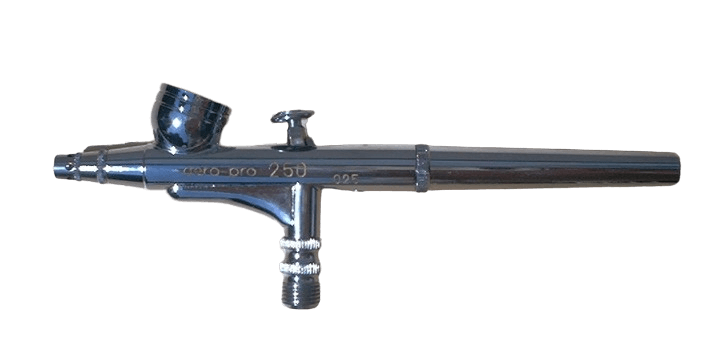
\includegraphics[width=0.8\textwidth]{assets/figures/etat_art/airbrush.png}
    \caption[Aérographe]{Aérographe \cite{airbrush_pics}\footnotemark}
\end{figure}
\footnotetext{\url{http://ingo-karkat.de/textilepainting/About\%20used\%20tools/index.html}}

L'aérographe repose sur l'effet venturi, l'air comprimé entraine le liquide à projeter dans l'embouchure assez fine de l'outil
transformant ce dernier en gouttelettes plus ou moins fines en fonction du réglage de l'aiguille de l'outil.

\begin{figure}[H]
    \centering
    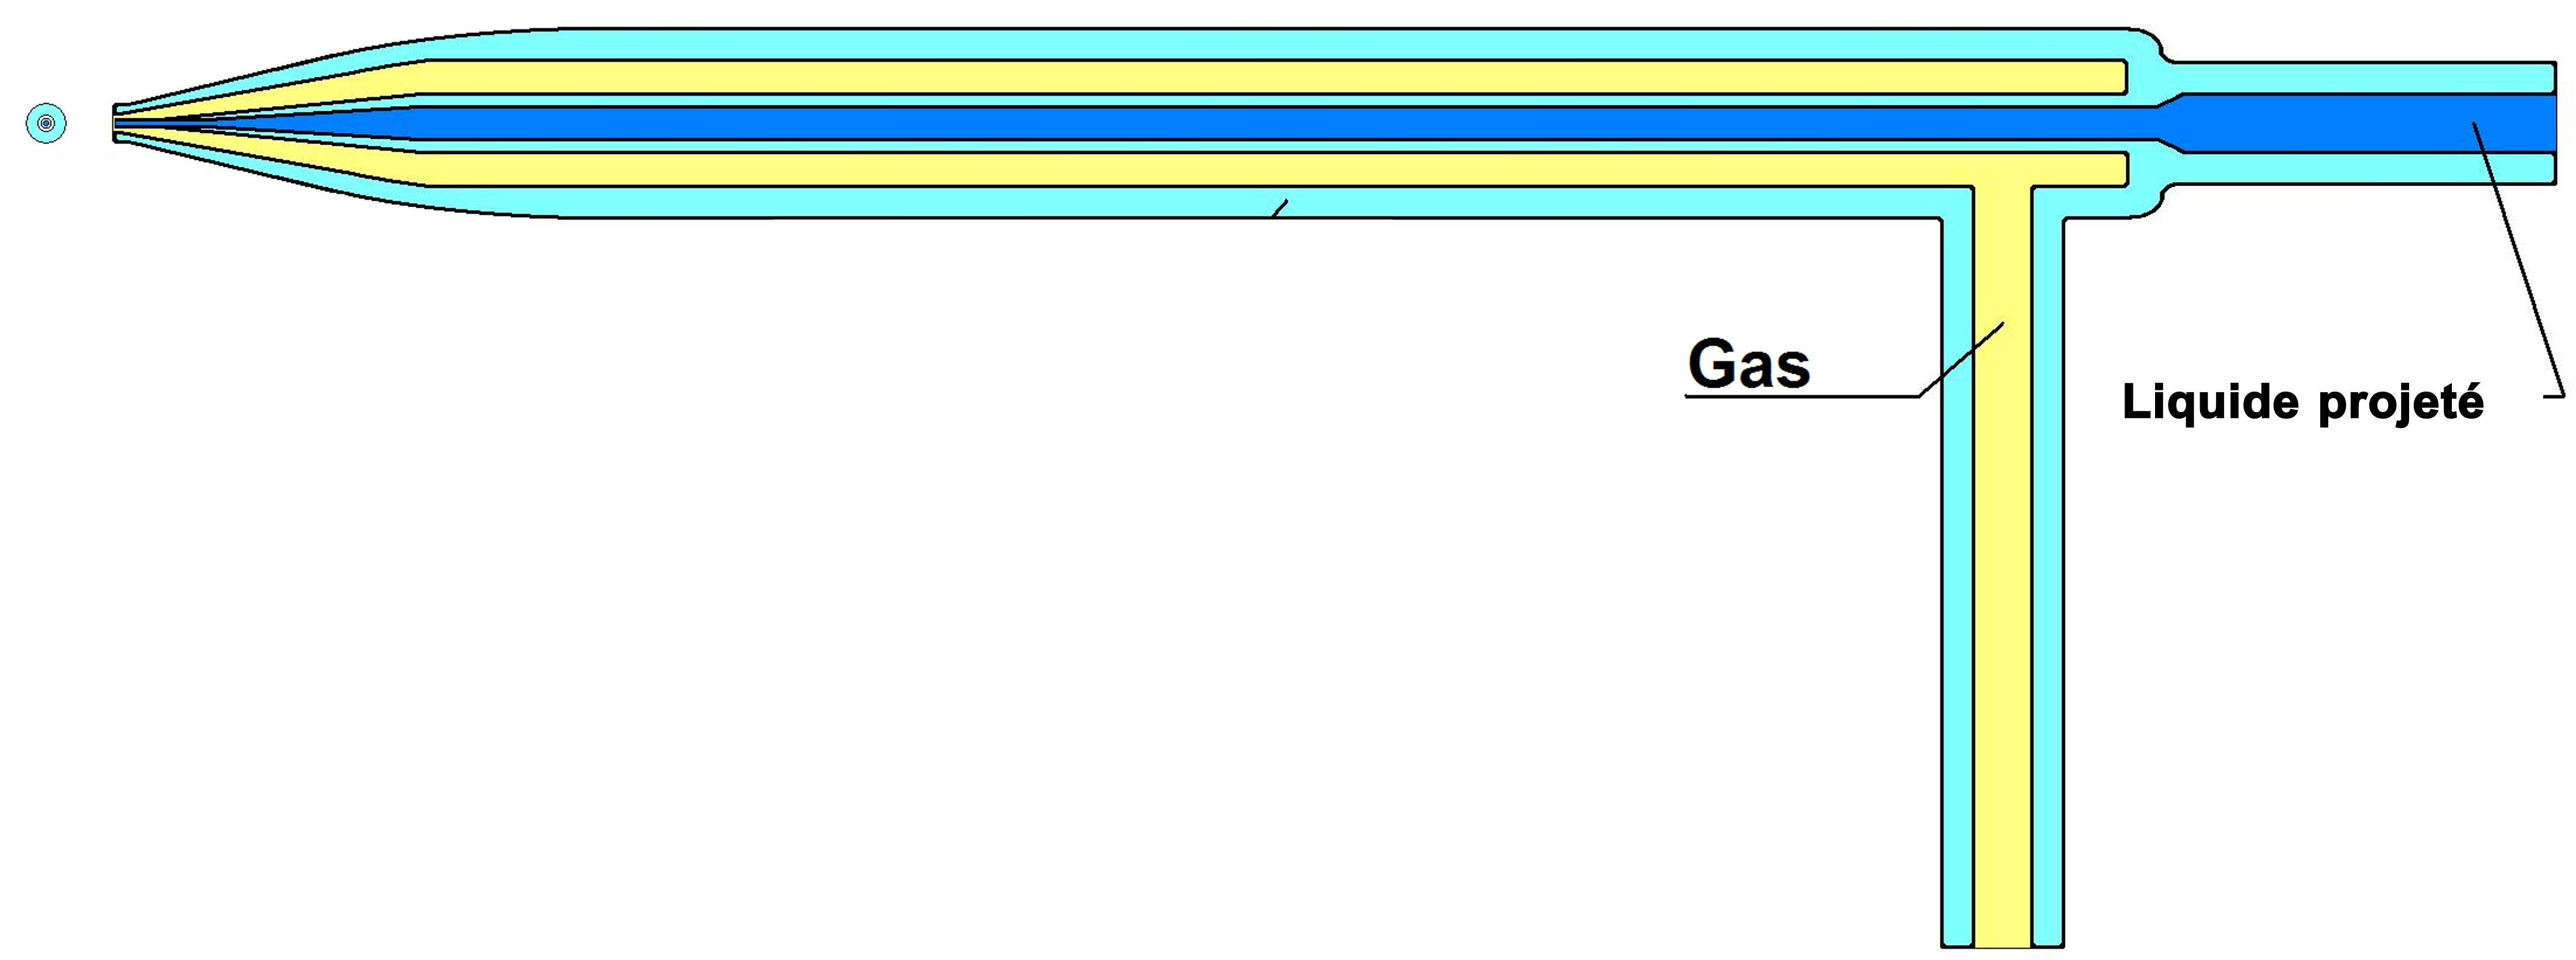
\includegraphics[width=0.6\textwidth]{assets/figures/etat_art/effet_venturi_aerographe.jpg}
    \caption[Effet venturi dans un aérographe]{Effet venturi dans aérographe \cite{venturi_airbrush}\footnotemark}
\end{figure}
\footnotetext{\url{https://upload.wikimedia.org/wikipedia/commons/1/1e/Nebulizzatoe\_concentrico.png}}

C'est la solution de projection sélectionnée dans la machine actuelle, il a pour avantage, d'être réglable assez finement
et de ne nécessiter qu'un compresseur, le critère de sélection principal lors du choix effectué par le concepteur de la machine
était la disponibilité de l'outil de façon rapide en l'empruntant à un tiers.

% Please add the following required packages to your document preamble:
% \usepackage[table,xcdraw]{xcolor}
% Beamer presentation requires \usepackage{colortbl} instead of \usepackage[table,xcdraw]{xcolor}
\begin{table}[H]
    \centering
    \begin{tabular}{|c|c|lll}
        \cline{1-2}
        Avantages                                                                                            & Inconvénients                                     &  &  & \\ \cline{1-2}
        \cellcolor[HTML]{67FD9A}Non influencé par l'environnement                                            & \cellcolor[HTML]{FD6864}Montage actuel capricieux &  &  & \\ \cline{1-2}
        \cellcolor[HTML]{67FD9A}Motorisable -\textgreater reproductible                                      & \cellcolor[HTML]{FFFFFF}                          &  &  & \\ \cline{1-2}
        \cellcolor[HTML]{67FD9A}Beaucoup de possibilités de modifier la brumisation                          & \cellcolor[HTML]{FFFFFF}                          &  &  & \\ \cline{1-2}
        \multicolumn{1}{|l|}{\cellcolor[HTML]{67FD9A}Possibilité de contrôler la composition de l'acrylique} & \multicolumn{1}{l|}{}                             &  &  & \\ \cline{1-2}
        \multicolumn{1}{|l|}{\cellcolor[HTML]{67FD9A}Bouton qui bloque l'air intégré}                        & \multicolumn{1}{l|}{}                             &  &  & \\ \cline{1-2}
    \end{tabular}
    \caption{Résumé des avantages et inconvénients de l'aérographe}
    \label{tab:aerographe_table}
\end{table}
\subsection{Atomiseurs pneumatiques}
Les atomiseurs pneumatiques reposent sur le même principe de fonctionnement que l'aérographe de la \autoref{section_aerographe}, donc avec effet
venturi et une aiguille pour régler la taille des gouttelettes.
\begin{figure}[H]
    \centering
    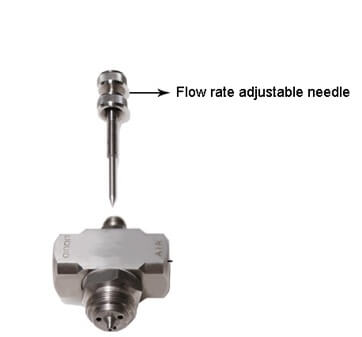
\includegraphics[width=0.5\textwidth]{assets/figures/etat_art/atomizing_nozzle.jpg}
    \caption[Buse d'atomisation pneumatique]{Buse d'atomisation pneumatique \autocite{photo_buse_atomisation}\footnotemark}
\end{figure}
\footnotetext{\url{https://www.nozzlespray.com/uploads/allimg/220310/atomizingfogspraynozzlefordisinfection.jpg}}

Ces buses d'atomisation à air comprimé sont utilisées dans l'industrie pour recouvrir des surfaces (peinture), nettoyer avec de l'eau, dans la confection d'aliments et bien d'autres:
\begin{figure}[H]
    \centering
    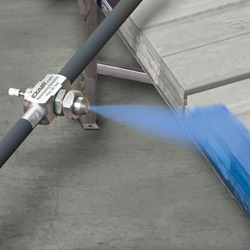
\includegraphics[width=0.5\textwidth]{assets/figures/etat_art/buse spray.jpeg}
    \caption[Exemple d'application d'une buse d'atomisation]{Exemple d'application d'une buse d'atomisation \autocite{exemple_application_buse}\footnotemark}
\end{figure}
\footnotetext{\url{https://english.exair.com/images/atom/IntMix-2\_250sq.png}}
\newpage
Elles permettent un choix de formes de projection assez vaste :
\begin{figure}[H]
    \centering
    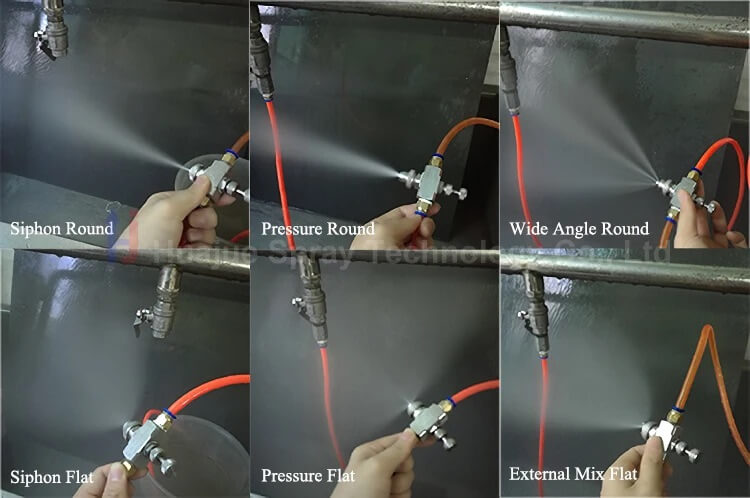
\includegraphics[width=0.9\textwidth]{assets/figures/etat_art/spray_patterns_example.jpeg}
    \caption[Exemples de différents "motifs" de spray]{Exemples de différents "motifs" de spray \autocite{Exemples_spray_patterns}\footnotemark}
\end{figure}
\footnotetext{\url{https://ae01.alicdn.com/kf/H428bb75251884fee8f19beffbbd38cfdp.jpg}}
C'est une piste de solution intéressante, elle fait déjà ses preuves dans plusieurs industries différentes.
L'activation du spray devra se faire de façon externe avec une électrovanne par exemple. Concernant la gestion de la taille
des gouttelettes, il faudra automatiser l'actionnement de l'aiguille. Concernant un point important pour ce type de matériel industriel, le prix,
des fournisseurs chinois pratiqueront des prix dans l'ordre de 10-20 frs, tandis que des fournisseurs traditionnels se situent plus dans les 300-800 frs. Il ne semble
pas y avoir de milieu de gamme.

% Please add the following required packages to your document preamble:
% \usepackage{graphicx}
% \usepackage[table,xcdraw]{xcolor}
% Beamer presentation requires \usepackage{colortbl} instead of \usepackage[table,xcdraw]{xcolor}
\begin{table}[H]
    \centering
    \resizebox{\textwidth}{!}{%
        \begin{tabular}{|c|c|lll}
            \cline{1-2}
            Avantages                                                                                            & Inconvénients                                                  &  &  & \\ \cline{1-2}
            \cellcolor[HTML]{67FD9A}Non influencé par l'environnement                                            & \cellcolor[HTML]{FD6864}Pas de bouton de blocage du flux d'air &  &  & \\ \cline{1-2}
            \cellcolor[HTML]{67FD9A}Motorisable -\textgreater reproductible                                      & \cellcolor[HTML]{FD6864}Classes de prix non régulières         &  &  & \\ \cline{1-2}
            \cellcolor[HTML]{67FD9A}Beaucoup de possibilités de modifier la brumisation                          & \cellcolor[HTML]{FFFFFF}                                       &  &  & \\ \cline{1-2}
            \multicolumn{1}{|l|}{\cellcolor[HTML]{67FD9A}Possibilité de contrôler la composition de l'acrylique} & \multicolumn{1}{l|}{}                                          &  &  & \\ \cline{1-2}
            \multicolumn{1}{|l|}{\cellcolor[HTML]{67FD9A}Solution utilisée dans l'industrie}                     & \multicolumn{1}{l|}{}                                          &  &  & \\ \cline{1-2}
            \multicolumn{1}{|l|}{\cellcolor[HTML]{67FD9A}Méthode de montage standardisée}                        & \multicolumn{1}{l|}{}                                          &  &  & \\ \cline{1-2}
        \end{tabular}%
    }
    \caption{Résumé des avantages et inconvénients de l'atomiseur pneumatique}
    \label{tab:atomiseur_pneumatique_table}
\end{table}

\newpage

\section{Liquides à projeter}
Dans cette partie de l'état de l'art, nous allons passer en revue les matériaux projetables sur les disques en acrylique.
La boîte de matériel du concepteur de la machine d'origine contenait déjà certains matériaux de cette section.

\subsection{}

\chapter{Améliorations}
\section{Porte}
Sur l'image ci-dessous, la porte dans son état original :
\begin{figure}[H]
    \centering
    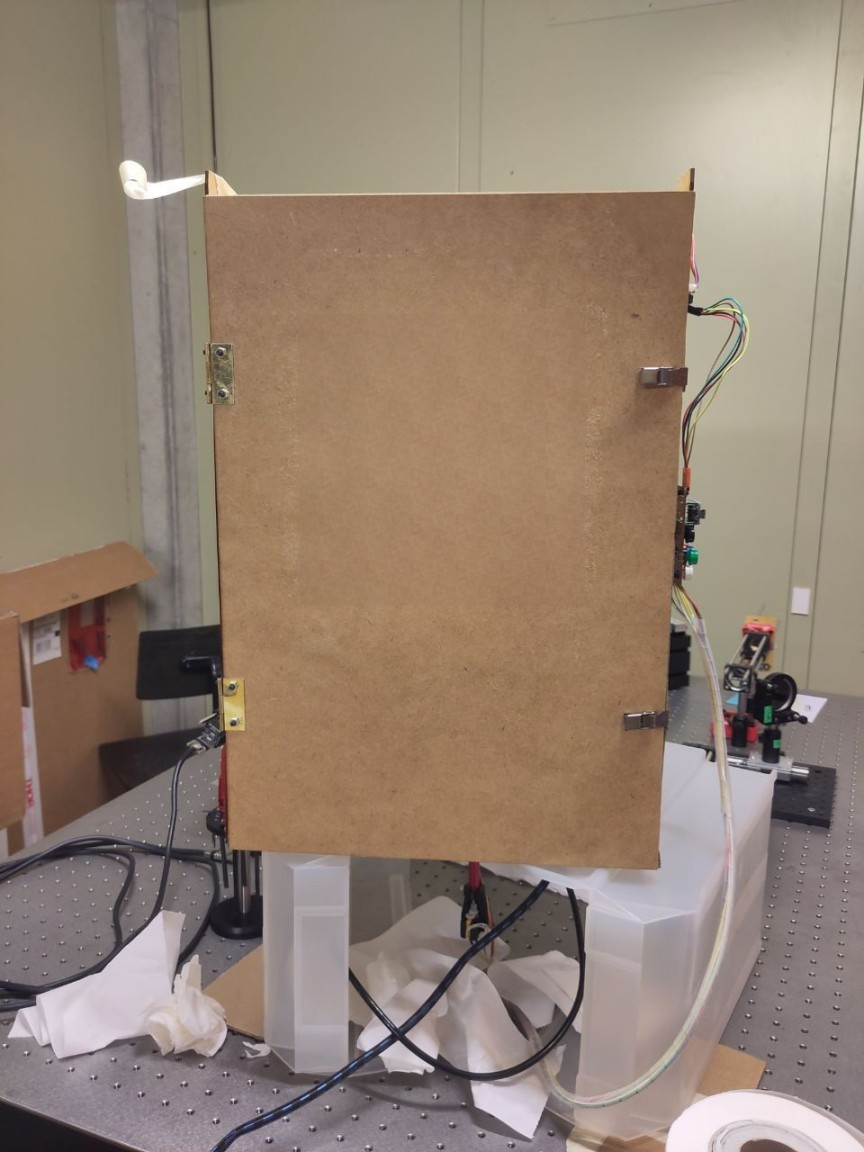
\includegraphics[width=0.5\textwidth]{assets/figures/ameliorations/porte_sans_fenetre.png}
    \caption{Photo de la porte avant modification}\label{photo porte}
\end{figure}

\newpage
Après une découpe dans le panneau de la porte, et le design de pièces de fixations et d'un chablon de perçage,
la porte est désormais équipée d'une fenetre:
\begin{figure}[H]
    \centering
    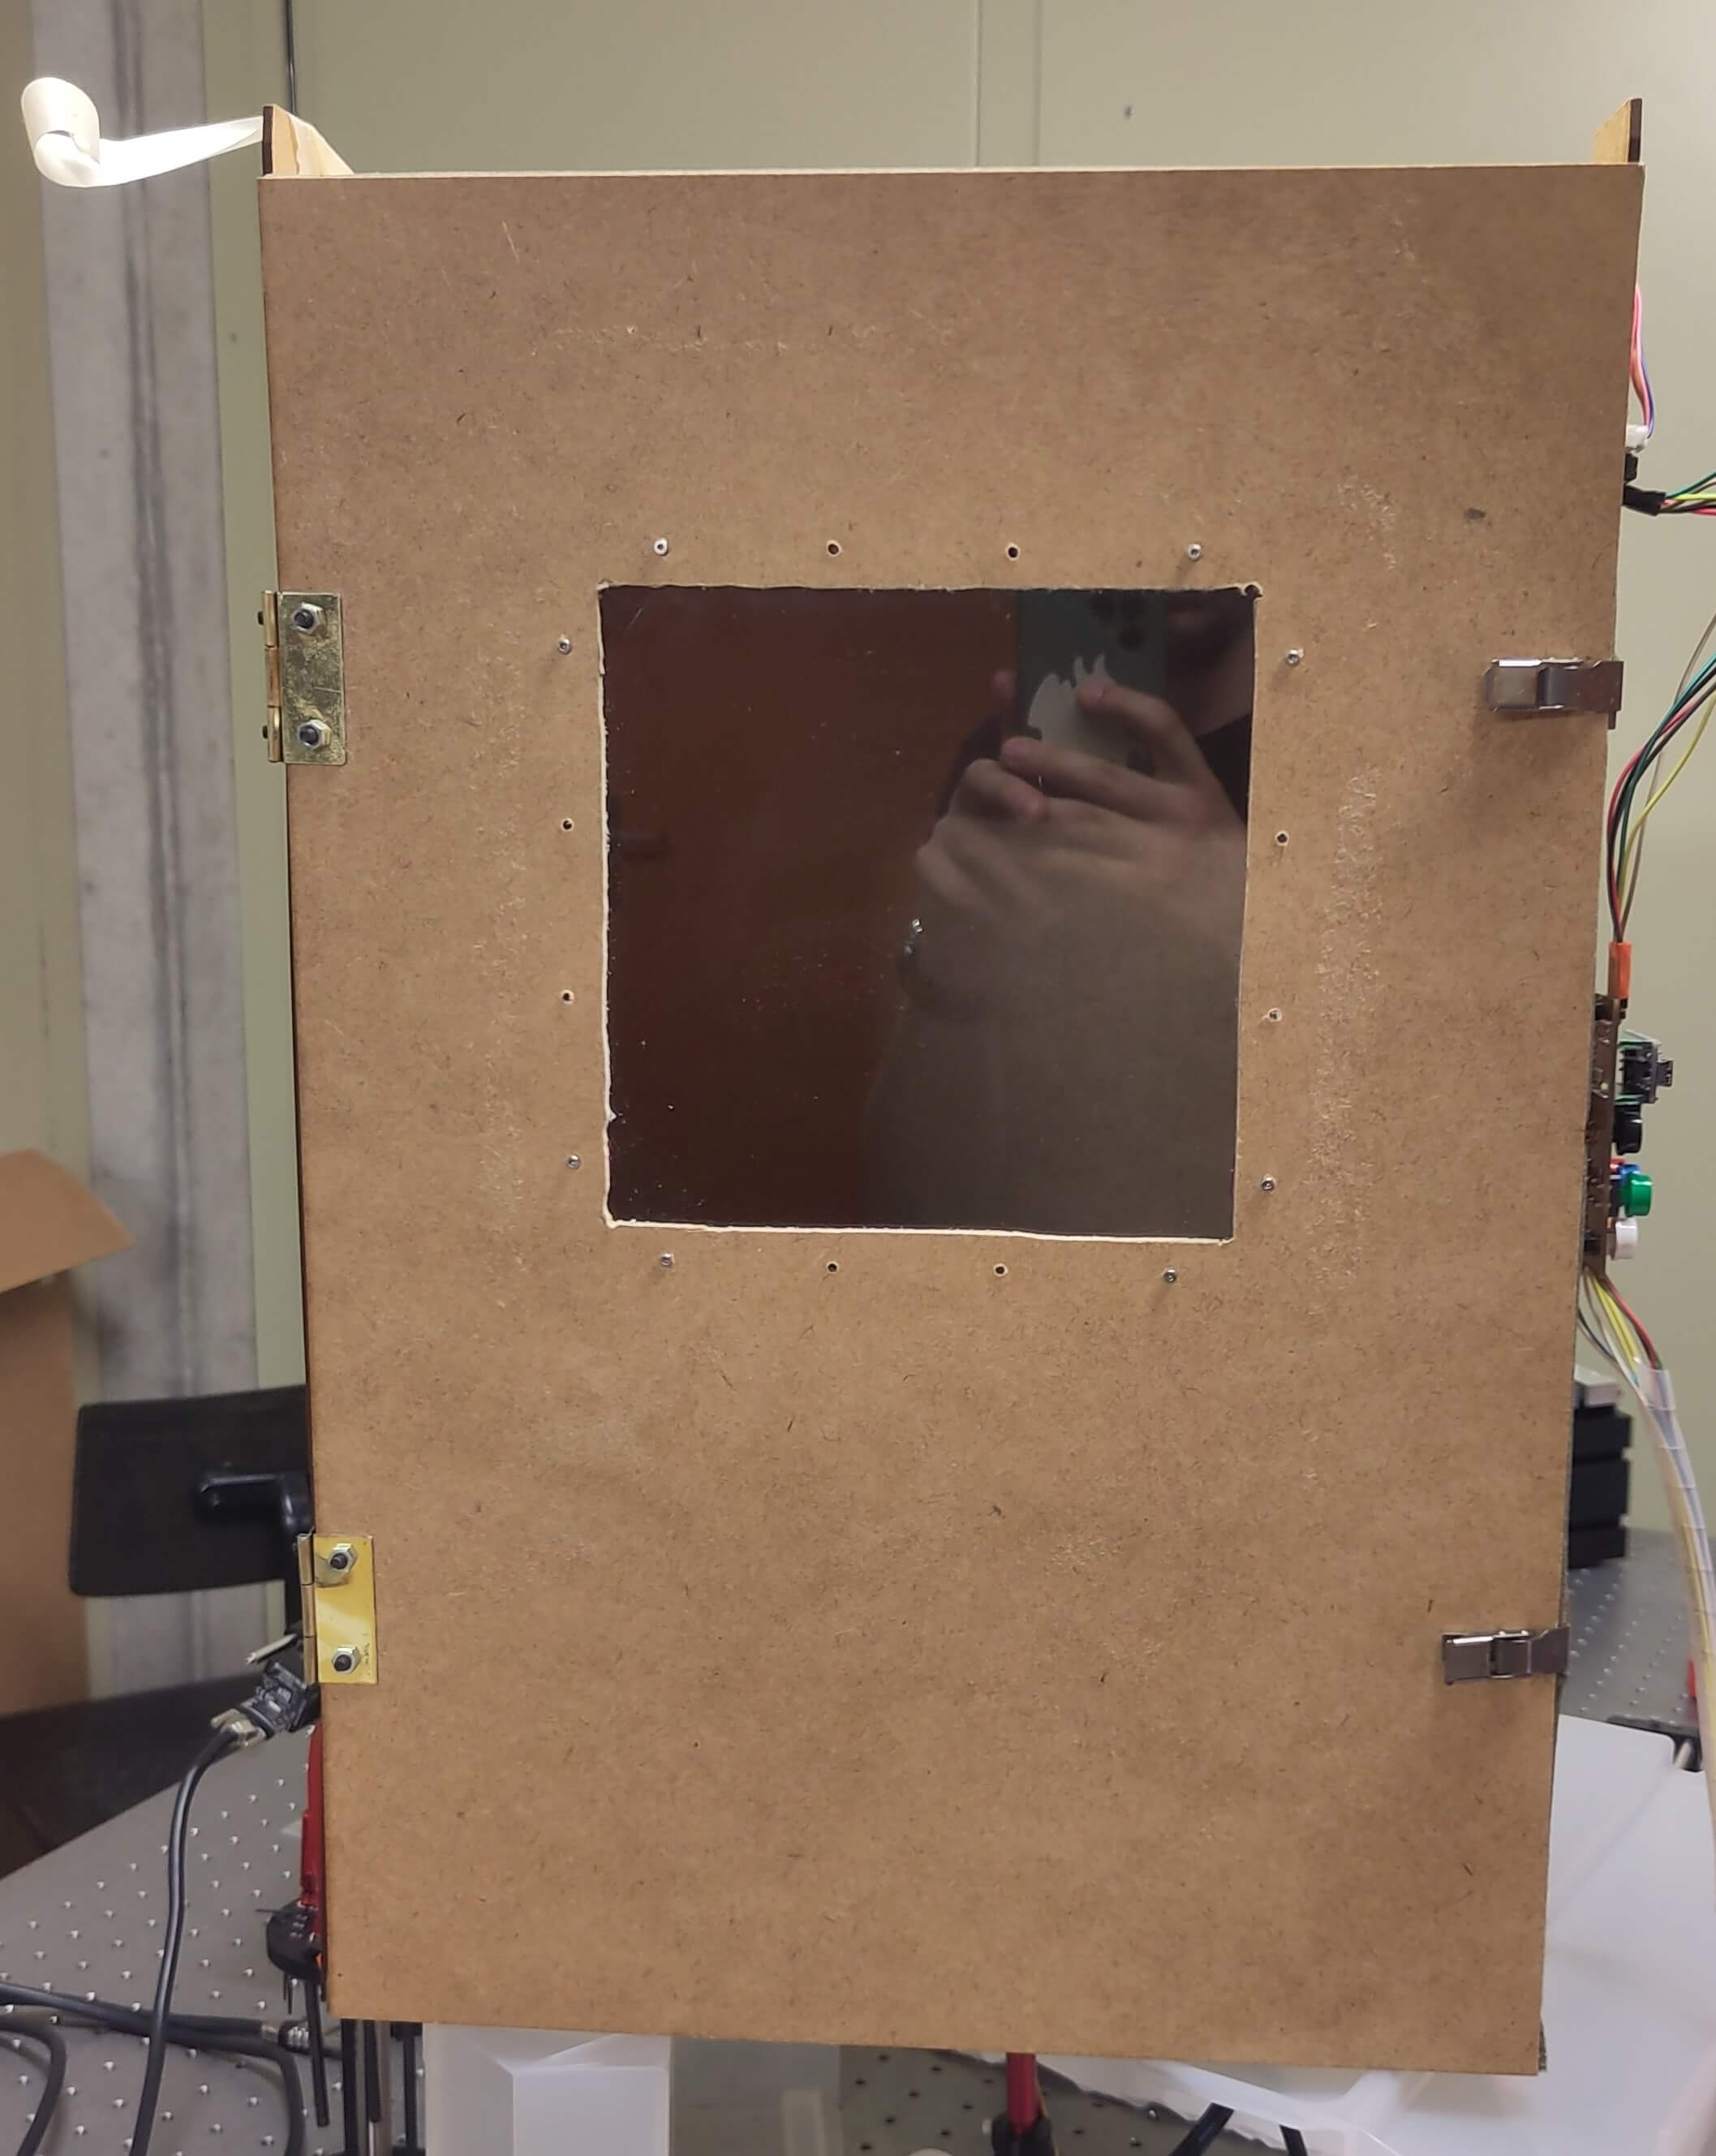
\includegraphics[width=0.5\textwidth]{assets/figures/ameliorations/porte_avec_fenetre.jpg}
    \caption{Photo de la porte après modification}\label{photo porte fenetre}
\end{figure}

La vitre est fixée à l'aide de petites broches vissées dans le bois :
\begin{figure}[H]
    \centering
    \begin{subfigure}{.5\textwidth}
        \centering
        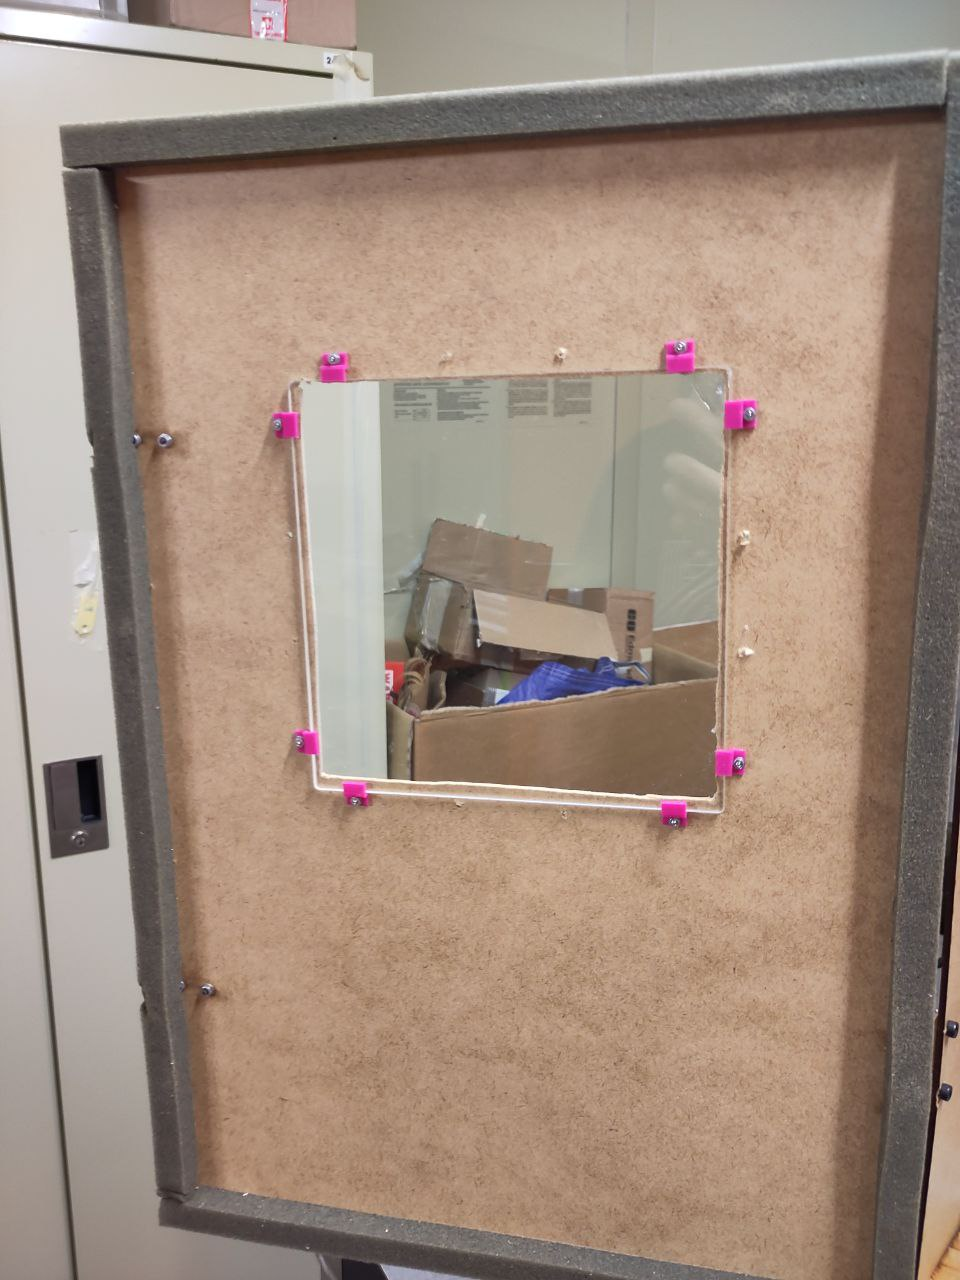
\includegraphics[width=1\linewidth,trim = 250 420 180 300, clip]{assets/figures/ameliorations/fixation_vitre.jpg}
        \caption{Vitre fixée}
        \label{fig:vitre_fixee}
    \end{subfigure}%
    \begin{subfigure}{.5\textwidth}
        \centering
        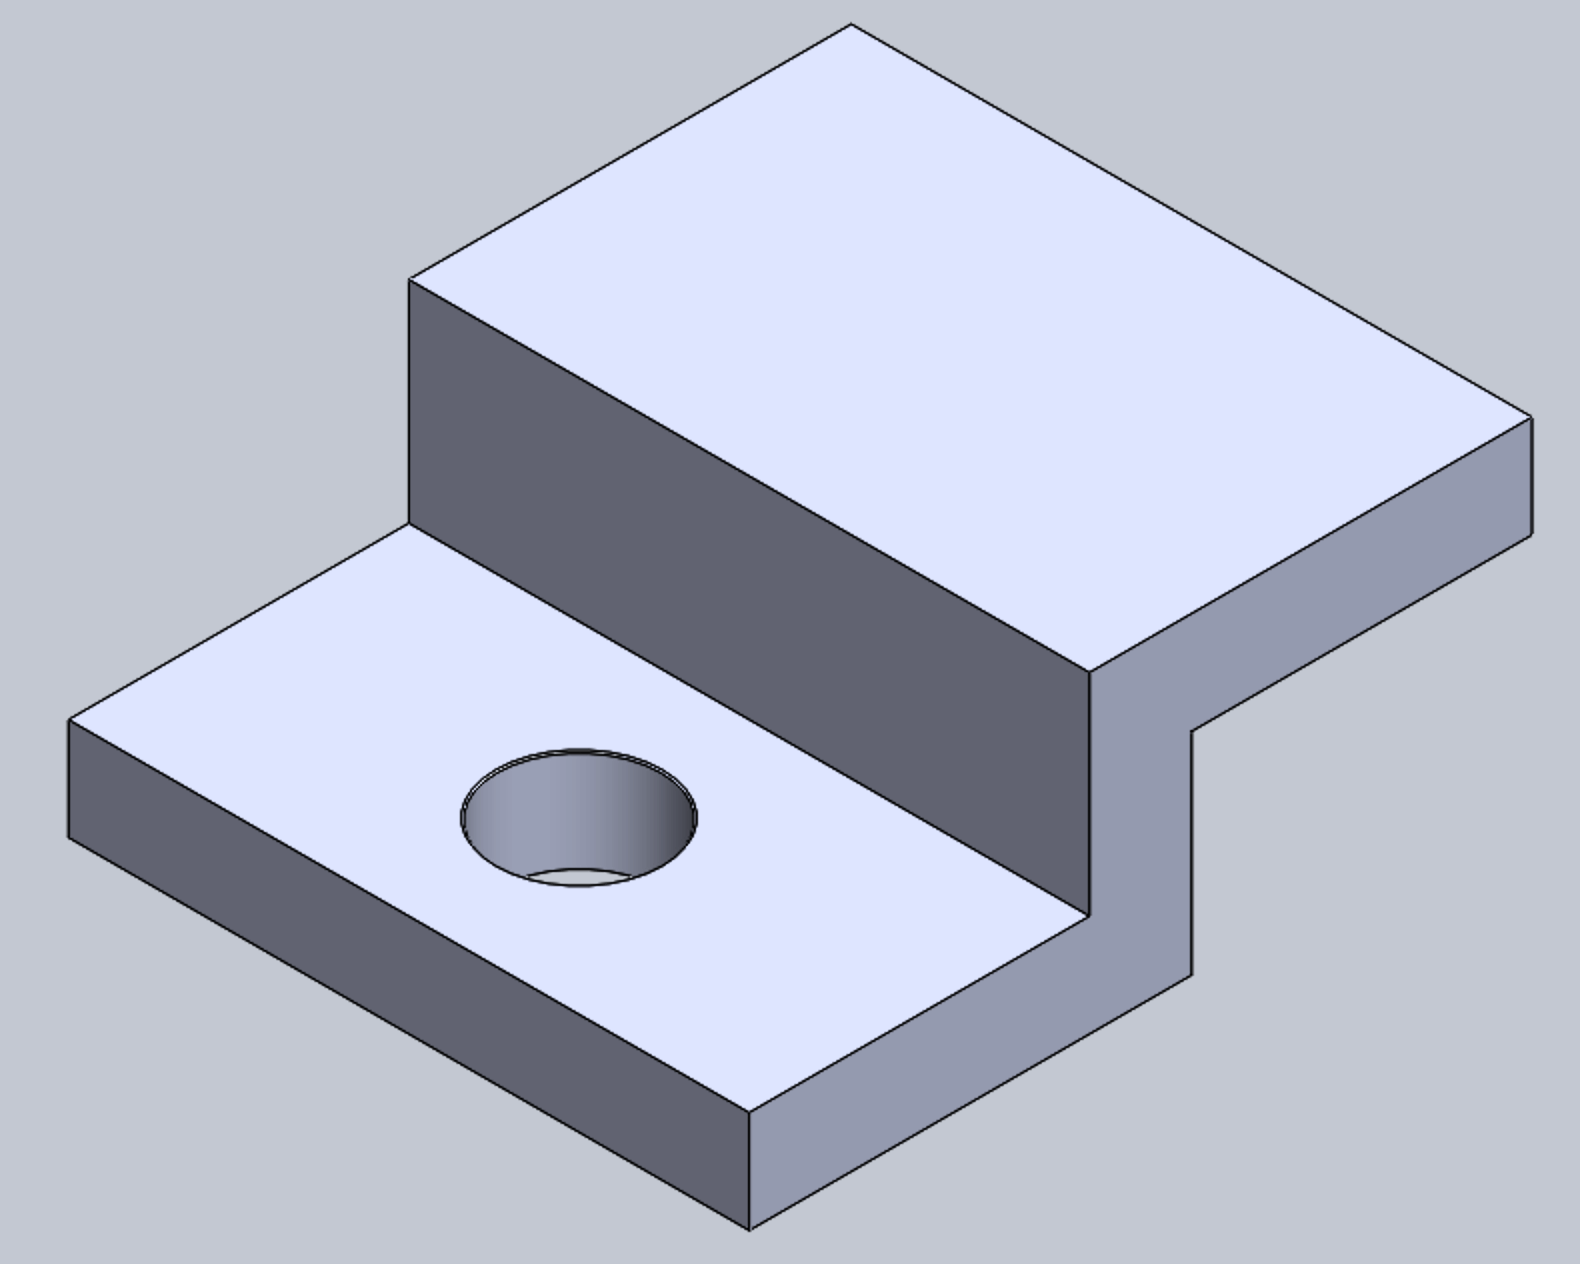
\includegraphics[width=.75\linewidth]{assets/figures/ameliorations/broche_vitre.png}
        \caption{Broche de fixation de la vitre}
        \label{fig:broche_fixation_vitre}
    \end{subfigure}
    \caption[Illustration de la fixation de la vitre]{Illustration de la fixation de la vitre}
    \label{fig:illu_vitre_porte}
\end{figure}
Le chablon pour les trous est trouvable dans l'\autoref{chablon_trous_vitre}.
\newpage
\section{Mesures}
\subsection{Problématique et situation d'origine}
Le procédé de mesure d'origine est sommaire et nécessite beaucoup de temps, en effet il convient de:
\begin{enumerate}
    \item Placer le disque dans le faisceau :
          \begin{figure}[H]
              \centering
              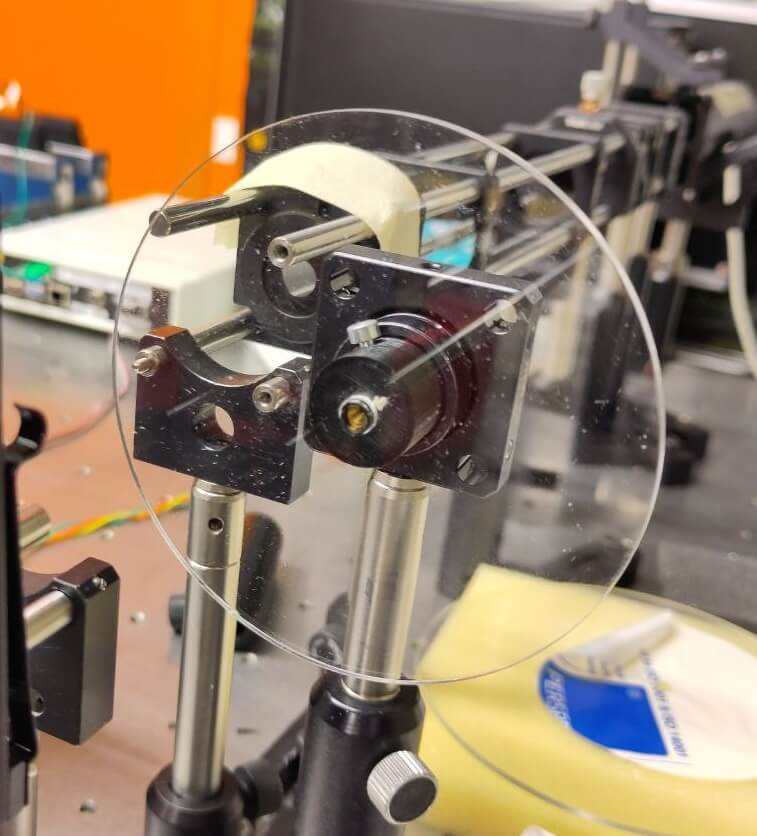
\includegraphics[width=0.5\textwidth]{assets/figures/ameliorations/disque_fixe.jpeg}
              \caption{Disque placé dans le faisceau}\label{fig:disque_fixe}
          \end{figure}

    \item Attendre quelques secondes que la mesure sur le logiciel soit stable:
          %   \begin{figure}[H]
          %       \centering
          %       
\includegraphics[width=0.5\textwidth]{assets/figures/Placeholder.jpeg}
          %       \caption{Placeholder}\label{Placeholder}
          %   \end{figure}

    \item Prendre la mesure l'enregistrer en format \textbf{.csv} avec le numéro de mesure.

    \item Tourner le disque d'un petit angle:
          \begin{figure}[H]
              \centering
              \includegraphics[width=0.5\textwidth,trim = 0 140 0 0, clip]{assets/figures/ameliorations/écran_rotation_manuelle.png}
              \caption{Rotation manuelle de l'écran}\label{fig:rotation_manuelle}
          \end{figure}
\end{enumerate}

Répéter en suite les étapes \textbf{2 à 4} pour autant de mesures qu'il le faut.
Dans le cadre de ce projet, plus il y a de données mieux c'est, il convient donc d'automatiser le
processus de prise de mesure au maximum pour pouvoir caractériser les écrans de turbulance facilement.

\subsection{Solution développée}
L'idée est de contrôler par ordinateur la prise de mesure ,interaction avec la caméra et la rotation de l'écran.
Après une petite configuration, l'utilisateur doit pouvoir laisser le système tourner et prendre les mesures nécessaires sans
interaction externe nécessaire.

\subsubsection{Caméra}

La caméra utilisée pour mesurer le front d'ondes est une \textbf{Thorlabs WFS40-7AR}:
\begin{figure}[H]
    \centering
    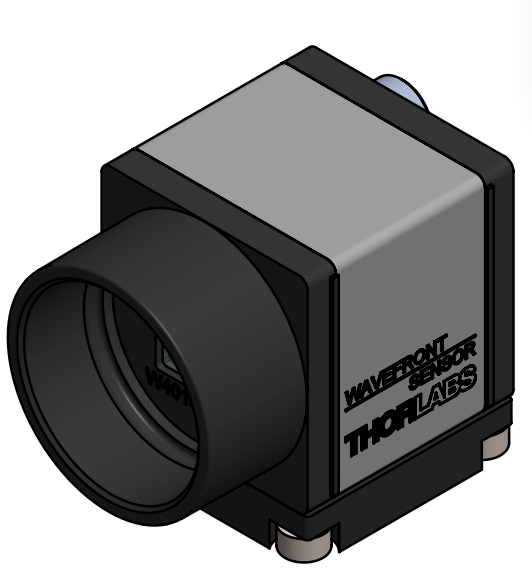
\includegraphics[width=0.4\textwidth]{assets/figures/ameliorations/thorlabs_40_7AR.png}
    \caption[Image de la caméra Thorlabs]{Image de la caméra Thorlabs \autocite{Camera_thorlabs_photo}}\label{fig:camera_thorlabs}
\end{figure}

Comme dit précédemment, il est possible d'intéragir avec la caméra à l'aide du logiciel fourni par Thorlabs, ce dernier permet de régler
la caméra, lire différentes mesures et visualiser le front d'onde.

La problématique était donc de trouver un moyen de communiquer avec la caméra, hors du logiciel dédié pour créer le programme de mesures.
Le manuel de la caméra, parle de la possibilité d'utiliser \textbf{LabView} pour accéder aux données et contrôler la caméra, en effet des
drivers spécifiques sont installés avec le programme de Thorlabs. Malheureusement cette solution ne fut pas retenue pour les raisons suivantes:

\begin{itemize}
    \item Le système de liscence de LabView à l'école est très contraignant.
    \item Mon système d'exploitation principal est MacOs (ainsi que celui de M. Jolissaint), LabView est peu compatible avec Mac et l'emulation de windows crash à cause des drivers.
\end{itemize}

Cela a donc porté mon regard sur l'utilisation de \textbf{Matlab}, et par chance, un utilisateur a développé une librairie Matlab permettant d'utiliser la caméra ! Cette ressource est disponible ici :
\url{https://www.mathworks.com/matlabcentral/fileexchange/116485-driver-for-thorlabs-shack-hartmann-wavefront-sensors-wfs}, elle a comme pré-requis, l'installation du logiciel de Thorlabs pour accéder aux drivers.

Il faut donc toujours utiliser un ordinateur sous windows, mais Matlab étant plus simple au niveau de ses licenses, il a été plus simple de juste travailler sur l'ordinateur du laboratoire.

\subsubsection{Rotation et translation de l'écran}
Pour faire tourner l'écran il fallait :
\begin{itemize}
    \item Un moyen de faire tourner l'écran.
    \item Faire communiquer l'ordinateur et le moyen de rotation.
\end{itemize}

Pour répondre au 1er besoin, nous avons utilisé un moteur pas-à-pas \textbf{28byj-48} :
\begin{figure}[H]
    \centering
    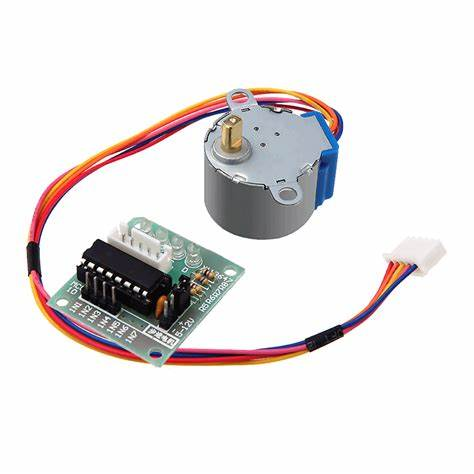
\includegraphics[width=0.5\textwidth]{assets/figures/ameliorations/stepper.jpeg}
    \caption[Moteur 28byj-48 pas-à-pas et son driver]{Moteur 28byj-48 pas-à-pas et son driver \autocite{photo_28byj-48}}
\end{figure}

Concernant la translation de l'écran, nous avons choisi d'utiliser un moteur pas-à-pas classique \textbf{36H22HM-0404A15-Z} avec un pignon et une crémaillère basée sur les
dimensions d'une courroie MXL classique\cite{dimensions_courroies_mxl}\footnotemark :
\begin{figure}[H]
    \centering
    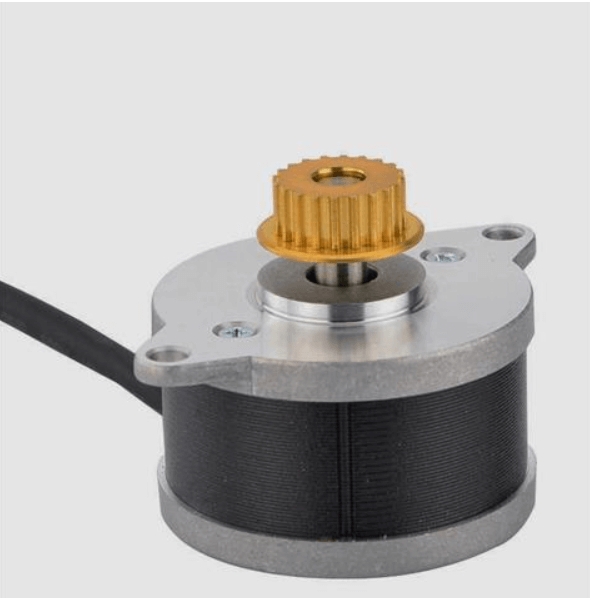
\includegraphics[width=0.3\textwidth]{assets/figures/ameliorations/36H22HM-0404A15-Z.png}
    \caption[Moteur 36H22HM-0404A15-Z]{Moteur pas-à-pas 36H22HM-0404A15-Z\autocite{moteur_translation_site}\footnotemark}
\end{figure}

\begin{figure}[H]
    \centering
    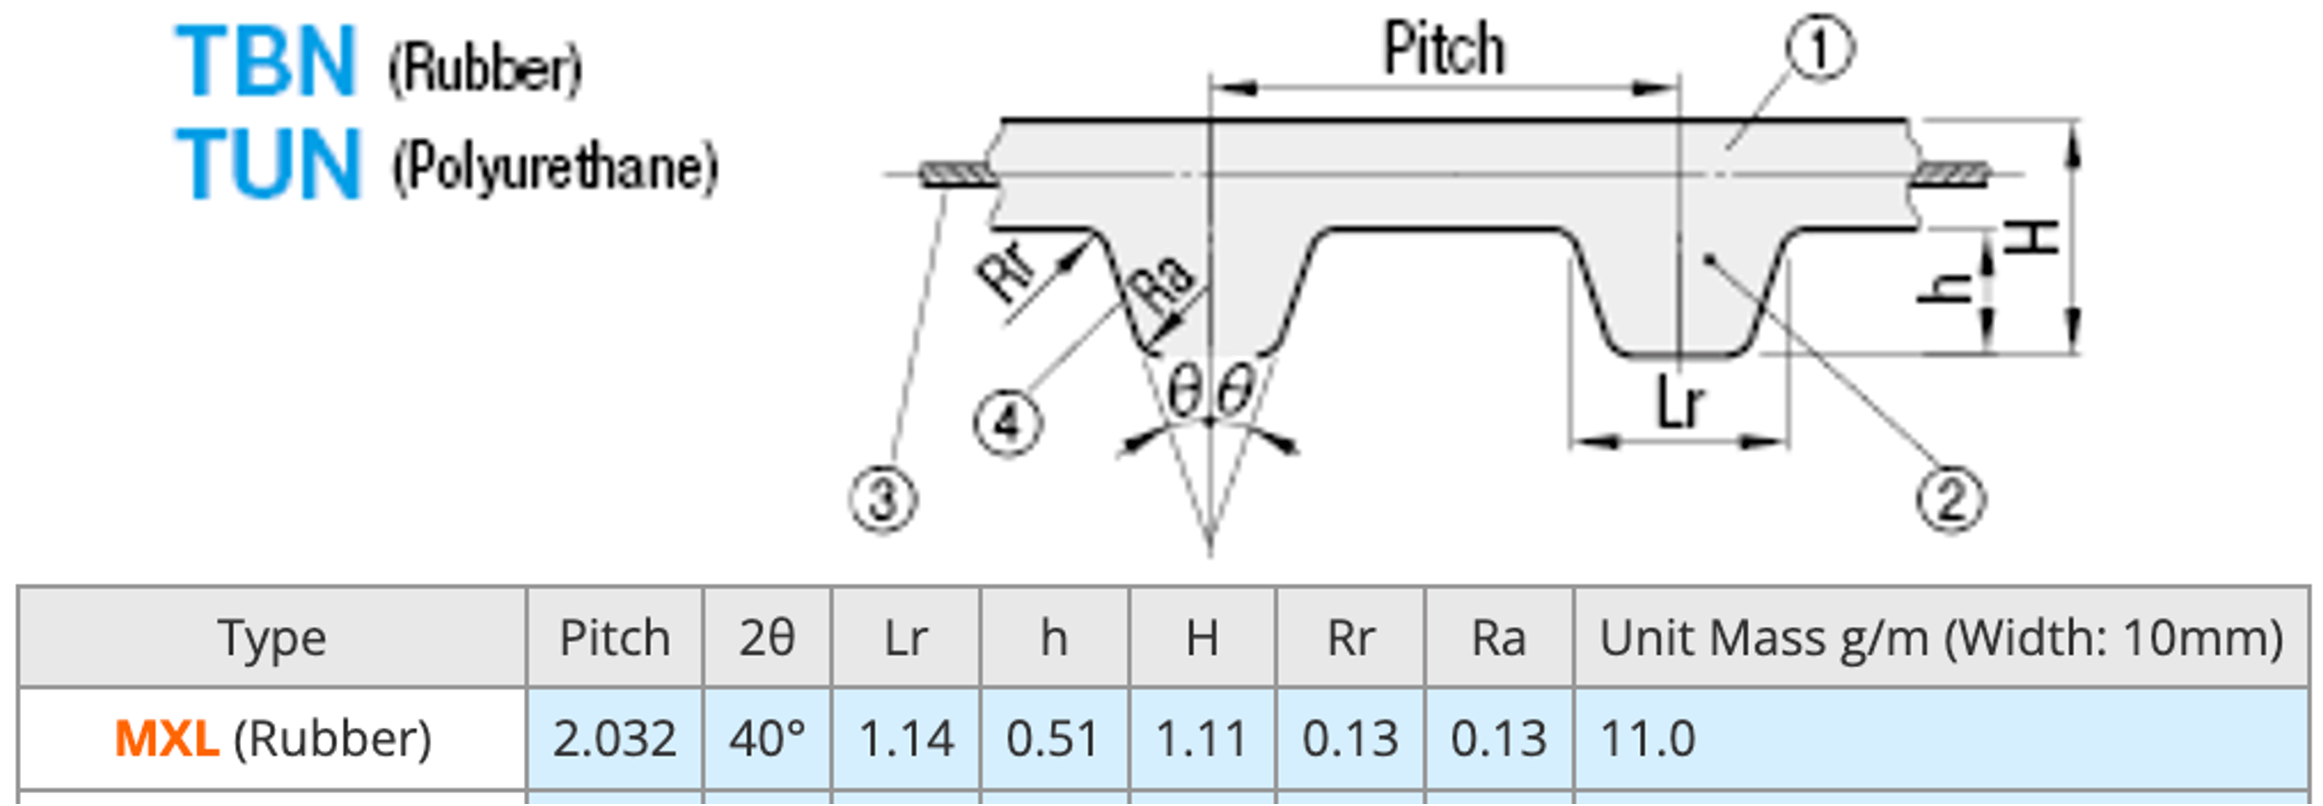
\includegraphics[width=0.8\textwidth]{assets/figures/ameliorations/dimensions_cremaillere.png}
    \caption[Dimensions crémaillère]{Dimensions crémaillère\autocite{dimensions_courroies_mxl}}
\end{figure}

\footnotetext{\url{https://uk.misumi-ec.com/vona2/detail/110302566050/}}
\footnotetext{\fullcite{moteur_translation_site}}



\subsubsection{Communication entre ordinateur et arduino}

Pour la communication entre l'ordinateur, le moteur de translation et celui de rotation, un arduino nano (clône) est utilisé :
\begin{figure}[H]
    \centering
    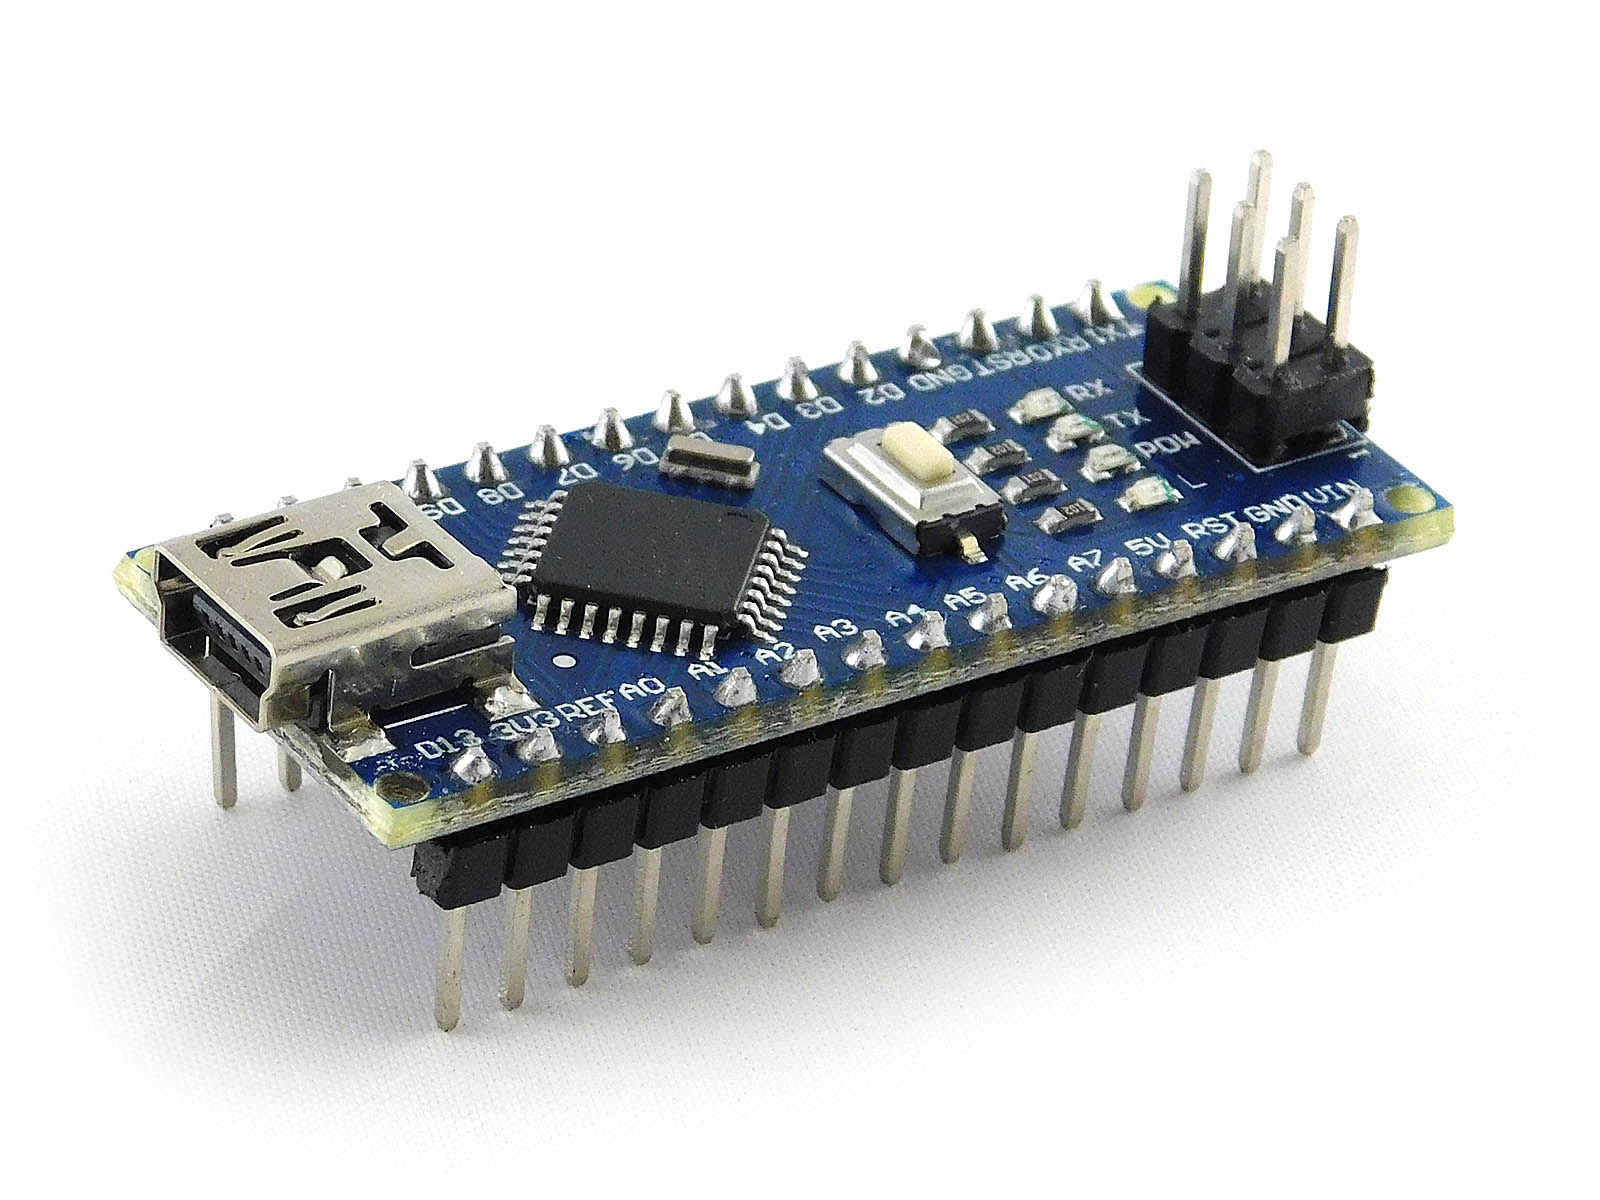
\includegraphics[width = 0.4\textwidth]{assets/figures/ameliorations/arduino_nano.jpg}
    \caption[Exemple de clône d'arduino nano]{Exemple de clône d'arduino nano \autocite{clone_nano}}
\end{figure}

Pour faire fonctionner le driver \textbf{ULN2003} du moteur de rotation à l'aide du microcontrôleur, la librairie \textbf{AccelStepper}\autocite{librairie_accelstepper} est utilisée.
Cette dernière permet entre autre, de régler l'accélération du moteur et le nombre de pas à effectuer, de démarrer le mouvement et de l'arrêter, savoir combiens de pas il reste à faire et bien plus,
la documentation du la librairie n'étant pas claire aux premiers abords un ressource complémentaire fut utilisée \autocite{AccelStepper_manual}.

Pour le moteur de translation, un driver \textbf{DRV8825} est employé :

\begin{figure}[H]
    \centering
    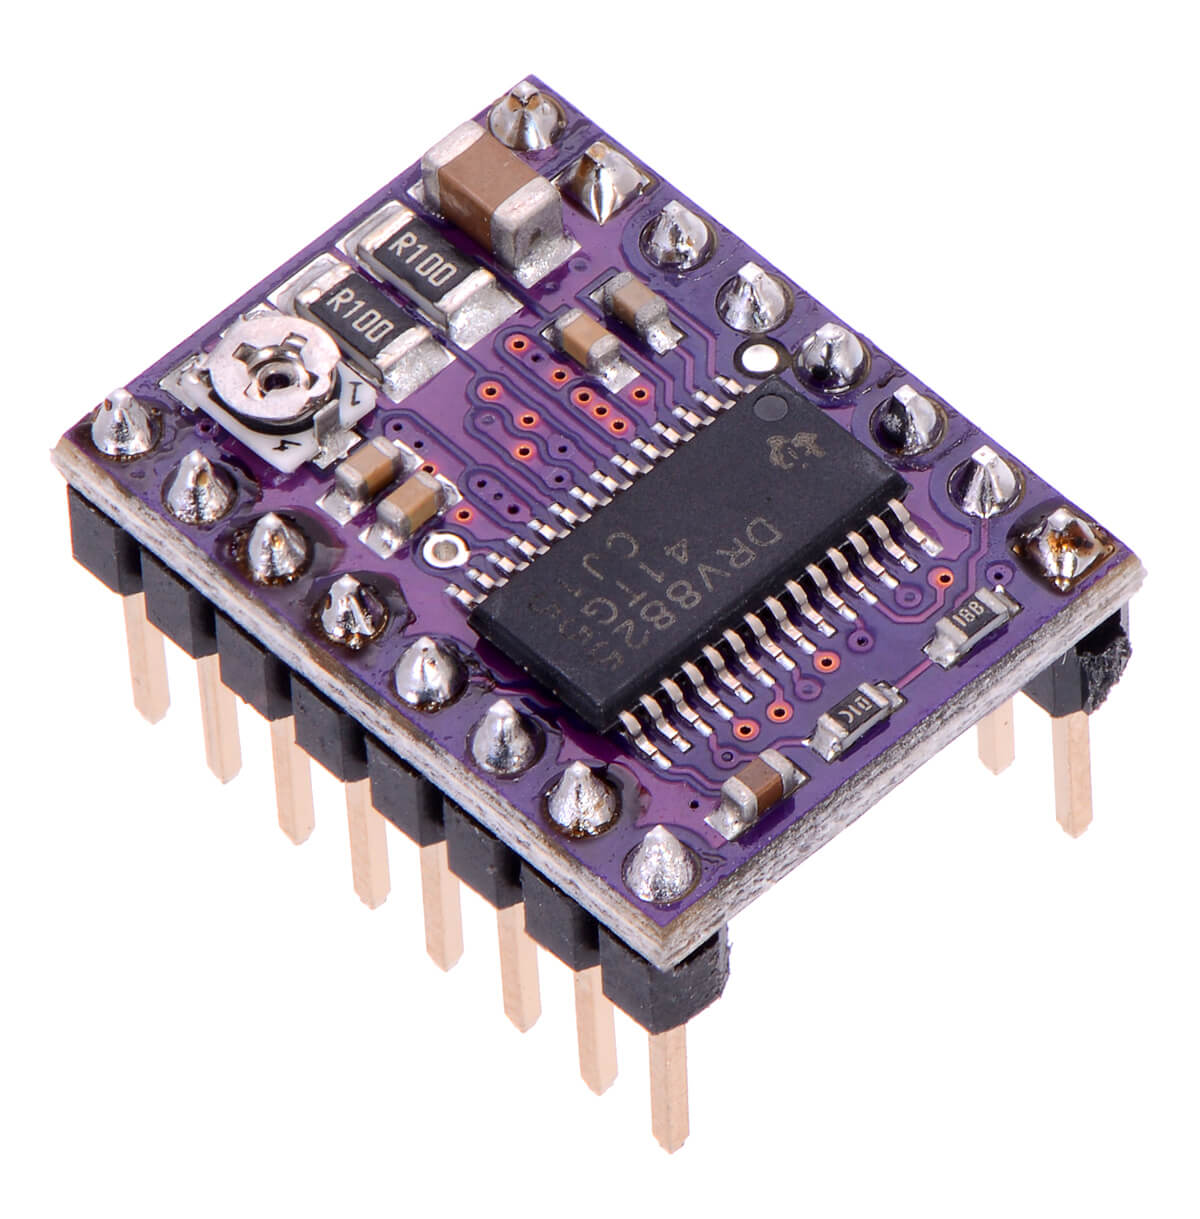
\includegraphics[width = 0.2\textwidth]{assets/figures/ameliorations/drv-8825.jpg}
    \caption[Driver DRV8825]{Driver DRV8825 \autocite{driver_DRV8825}\footnotemark}
\end{figure}
\footnotetext{\fullcite{driver_DRV8825}}
Ce dernier est piloté à l'aide de la librairie \textbf{StepperDriver}\cite{stepperDriver_lib}\footnotemark.

\footnotetext{\fullcite{stepperDriver_lib}}

La communication de matlab au microcontrôleur se fait via interface serial usb !
Le principe du protocole de communication est le suivant :
\begin{figure}[H]
    \centering
    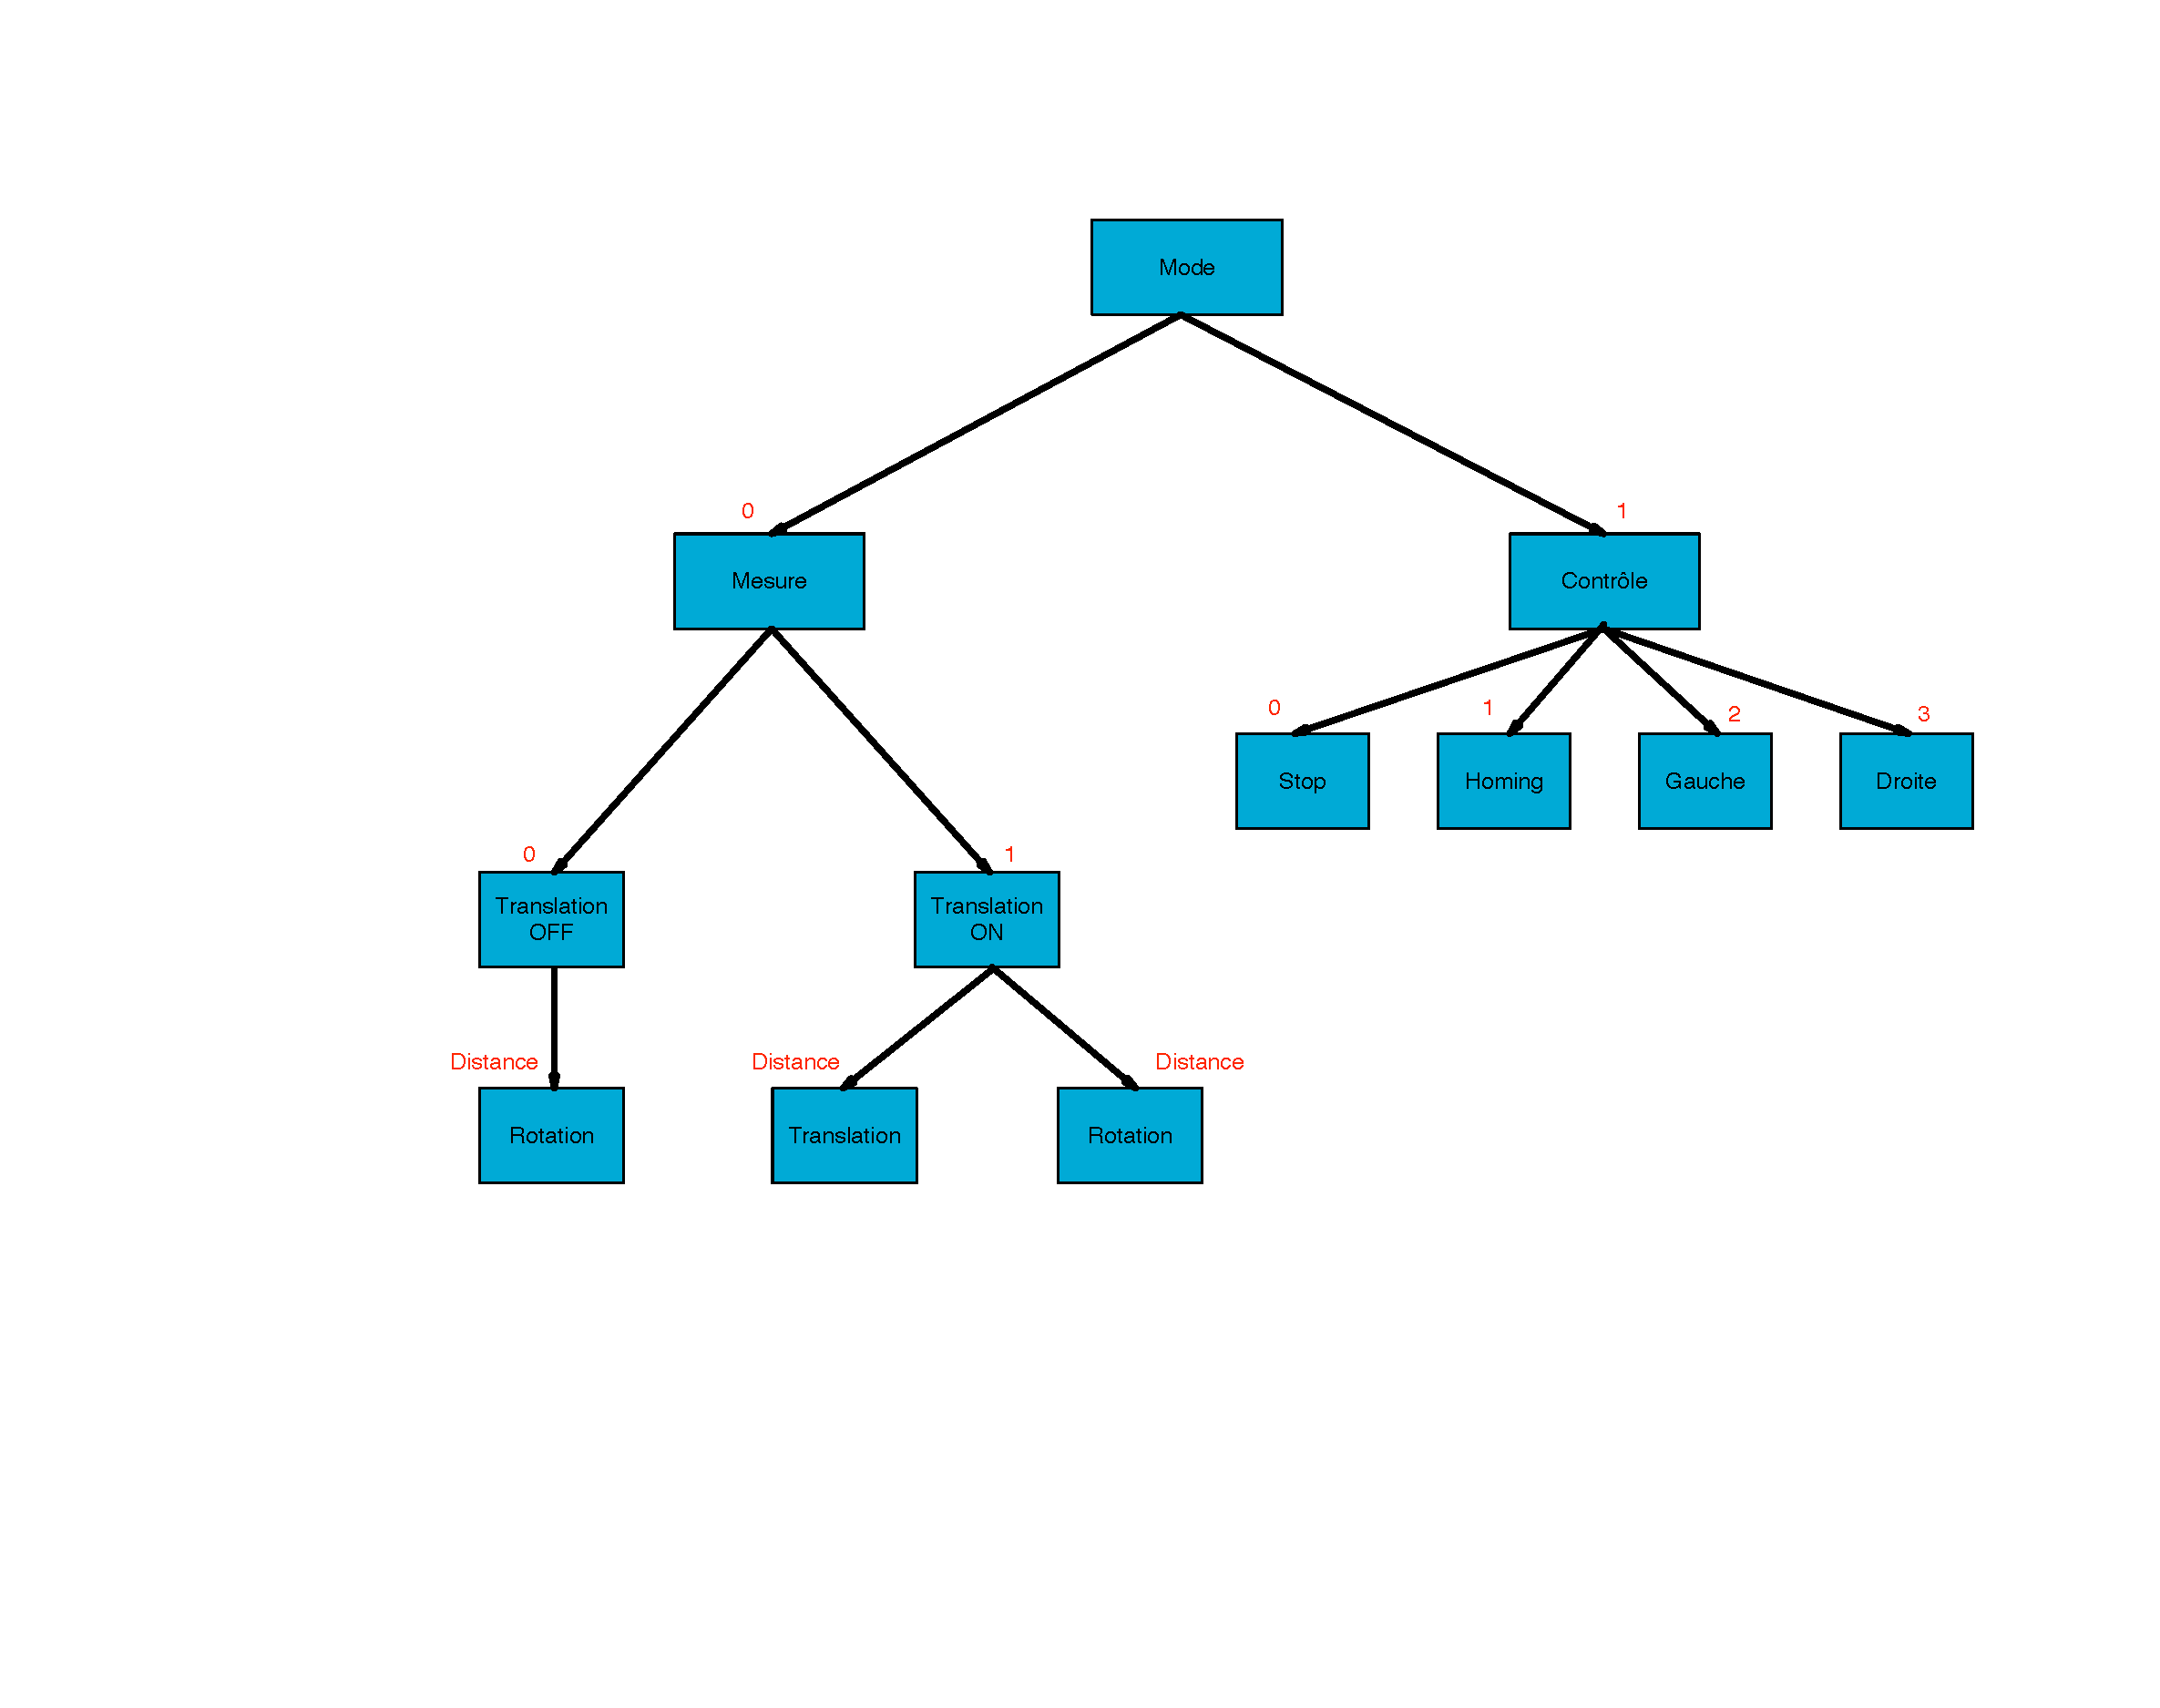
\includegraphics[page = 1, width = \textwidth, trim = {7cm 9cm 2cm 3cm},clip]{assets/figures/ameliorations/trame_comm.pdf}
    \caption[Structure de communication]{Structure de communication sous forme de choix ( en \color{red} rouge \color{black} = valeur dans la trame)}
\end{figure}
Sous forme de trame cela donne donc :
\begin{figure}[H]
    \centering
    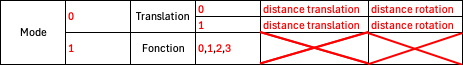
\includegraphics[width = 0.8\textwidth]{assets/figures/ameliorations/trame comm.png}
    \caption[Trame ordinateur <-> arduino mesure]{Trame ordinateur <-> arduino mesure( en \color{red} rouge \color{black} = valeur dans la trame)}
\end{figure}

Donc par exemple pour déclencher un homing la trame envoyée sera :
\begin{figure}[H]
    \centering
    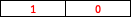
\includegraphics[scale = 1.3]{assets/figures/ameliorations/trame_homing.png}
    \caption[Trame homing]{Trame de homing}
\end{figure}
Ou pour effectuer une rotation de 130 pas et une translation de 150 pas (si on a fait un tour complet d'écran), la trame est la suivante:
\begin{figure}[H]
    \centering
    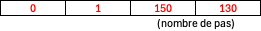
\includegraphics[scale = 1.2]{assets/figures/ameliorations/trame_translation_rotation.png}
    \caption[Trame translation rotation]{Trame de translation et de rotation pour mesure de l'écran\label{fig:trame_trans_rota}}
\end{figure}

Les trames sont quant à elles envoyées dans le bus serial sous forme de string de valeurs séparées par des virgules, par exemple pour la trame
de la \autoref{fig:trame_trans_rota} cela donnerait: \textbf{0,1,150,130}.

L'arduino qui reçoit ces instructions fonctionne sous le principe suivant :

\begin{figure}[H]
    \centering
    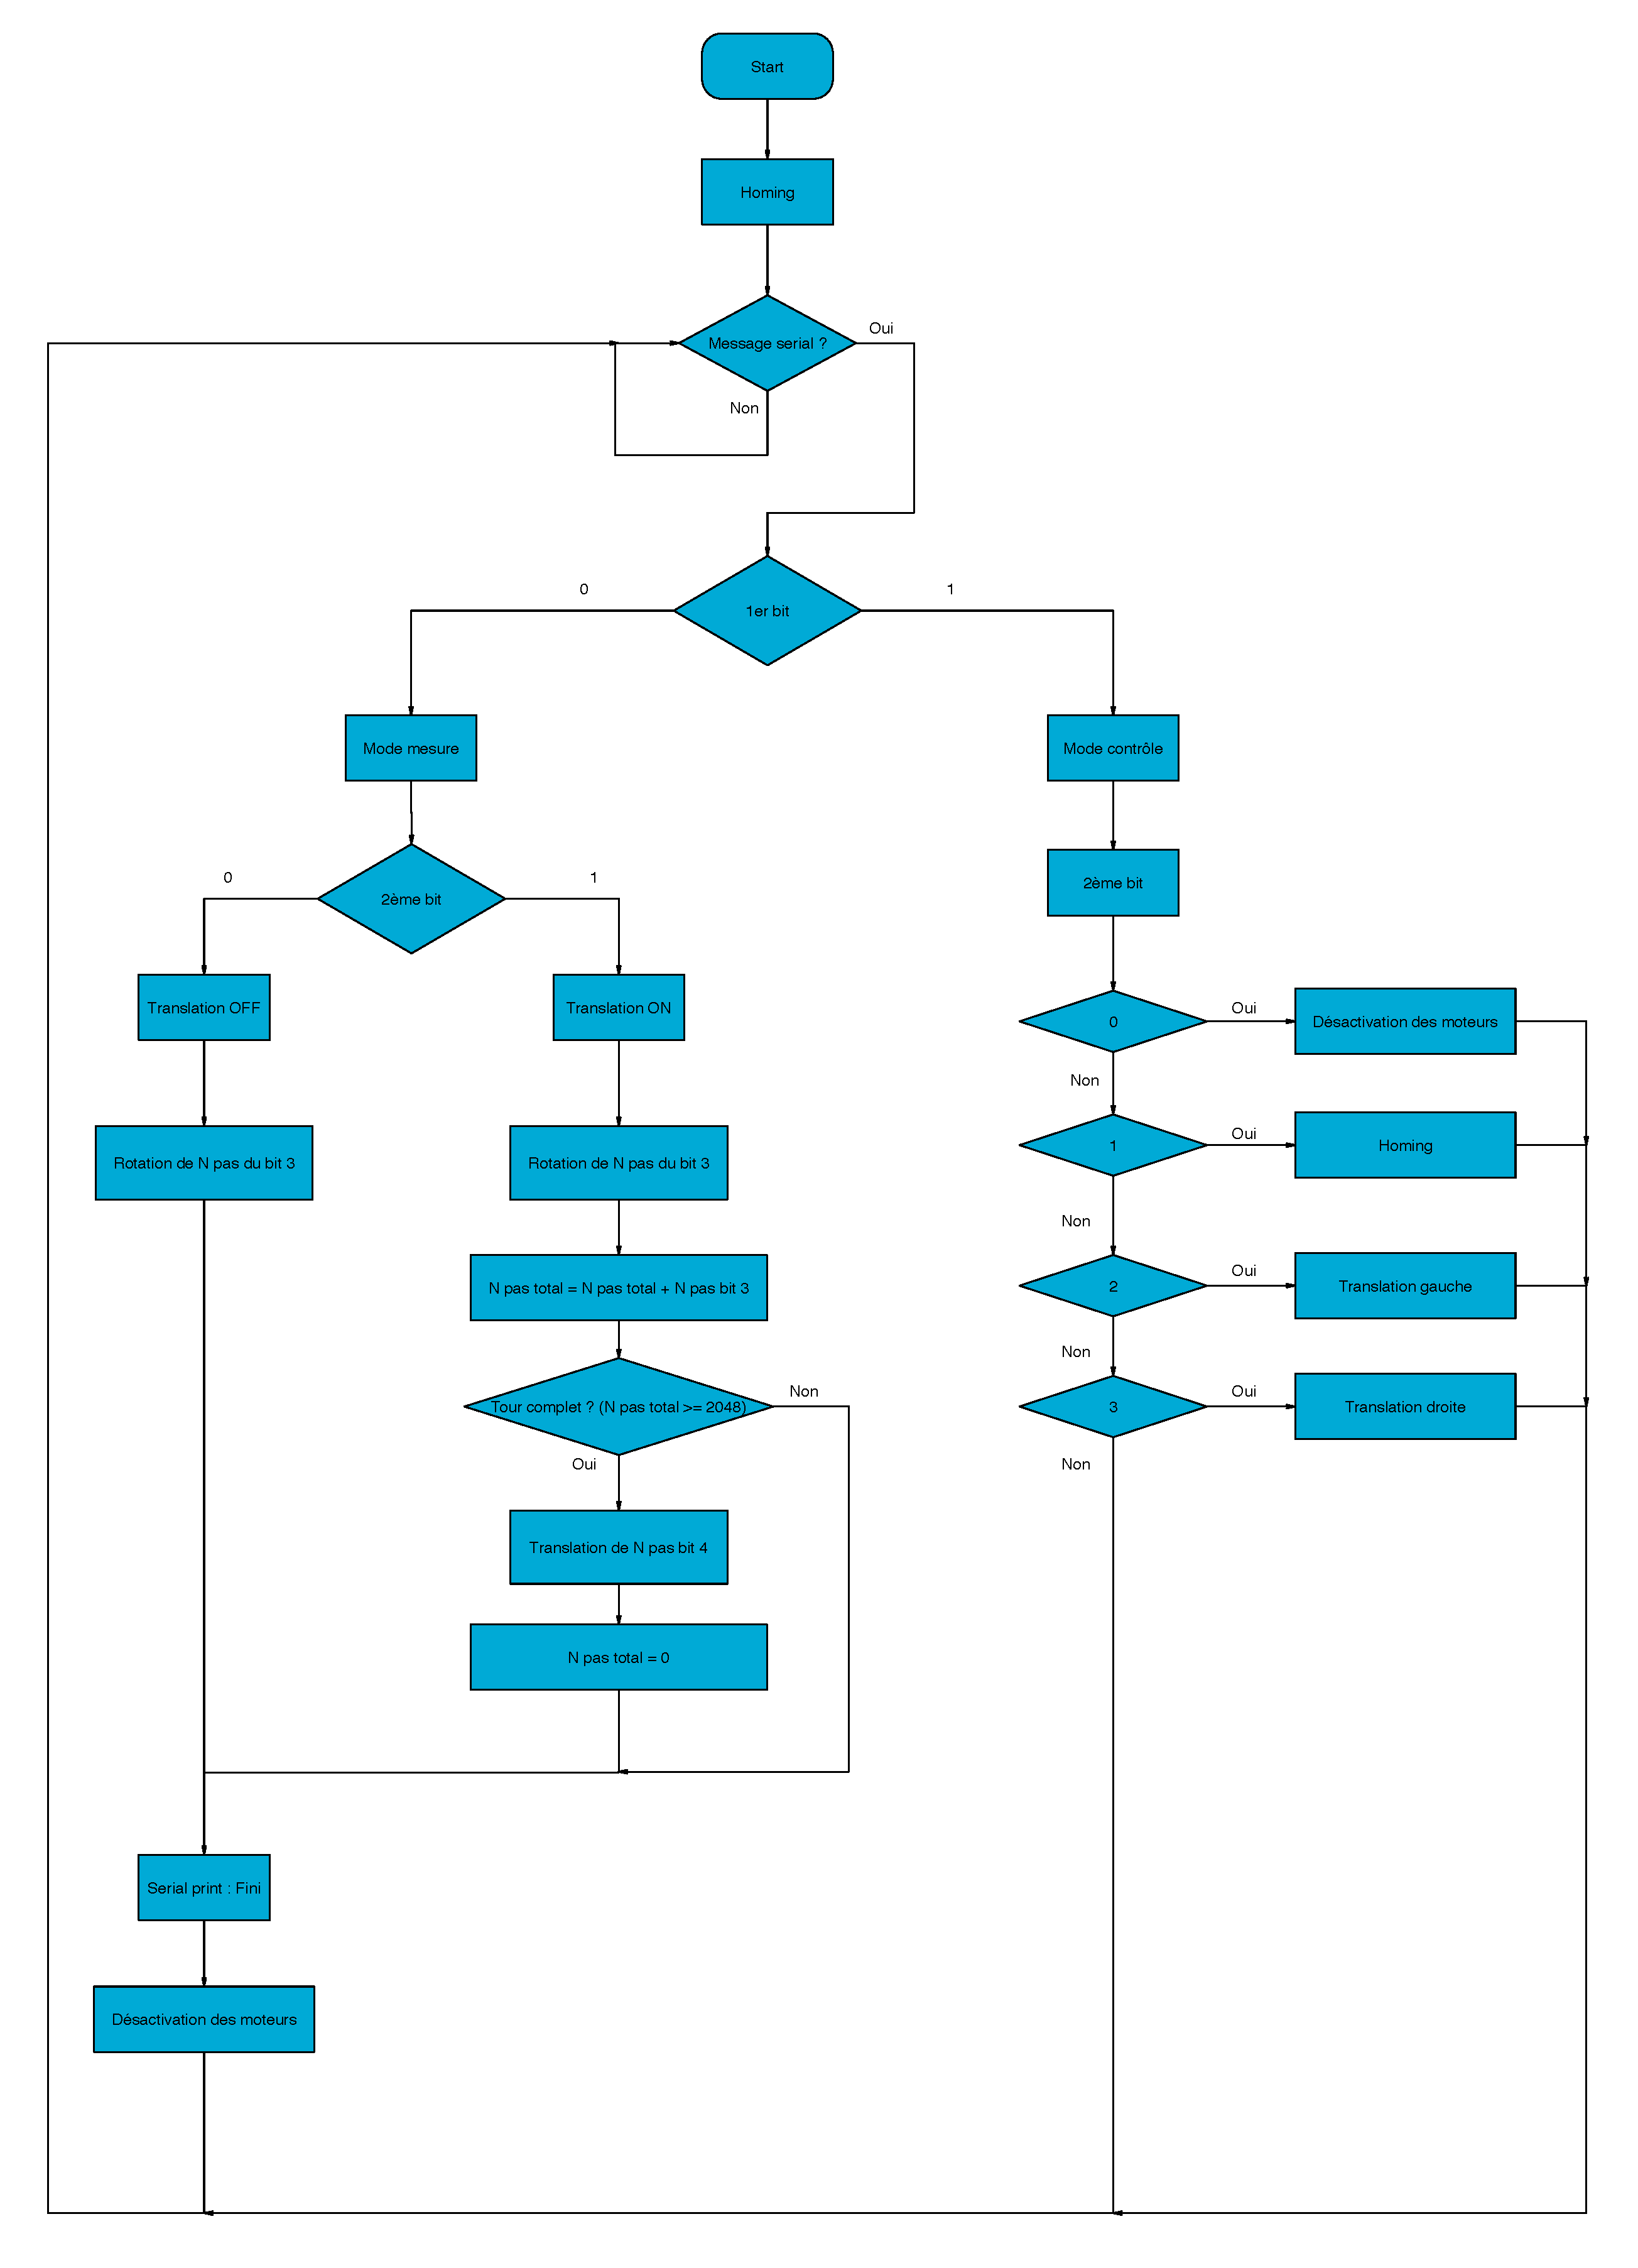
\includegraphics[width = \textwidth]{assets/figures/ameliorations/Structogramme_arduino.pdf}
    \caption[Structogramme programme microcontrôleur de mesure]{Structogramme programme microcontrôleur de mesure}
\end{figure}
Le code de l'arduino est consultable en \autoref{code:arduino_mesure}.

\newpage
\subsection{PCB système de mesure}

\begin{figure}[H]
    \centering
    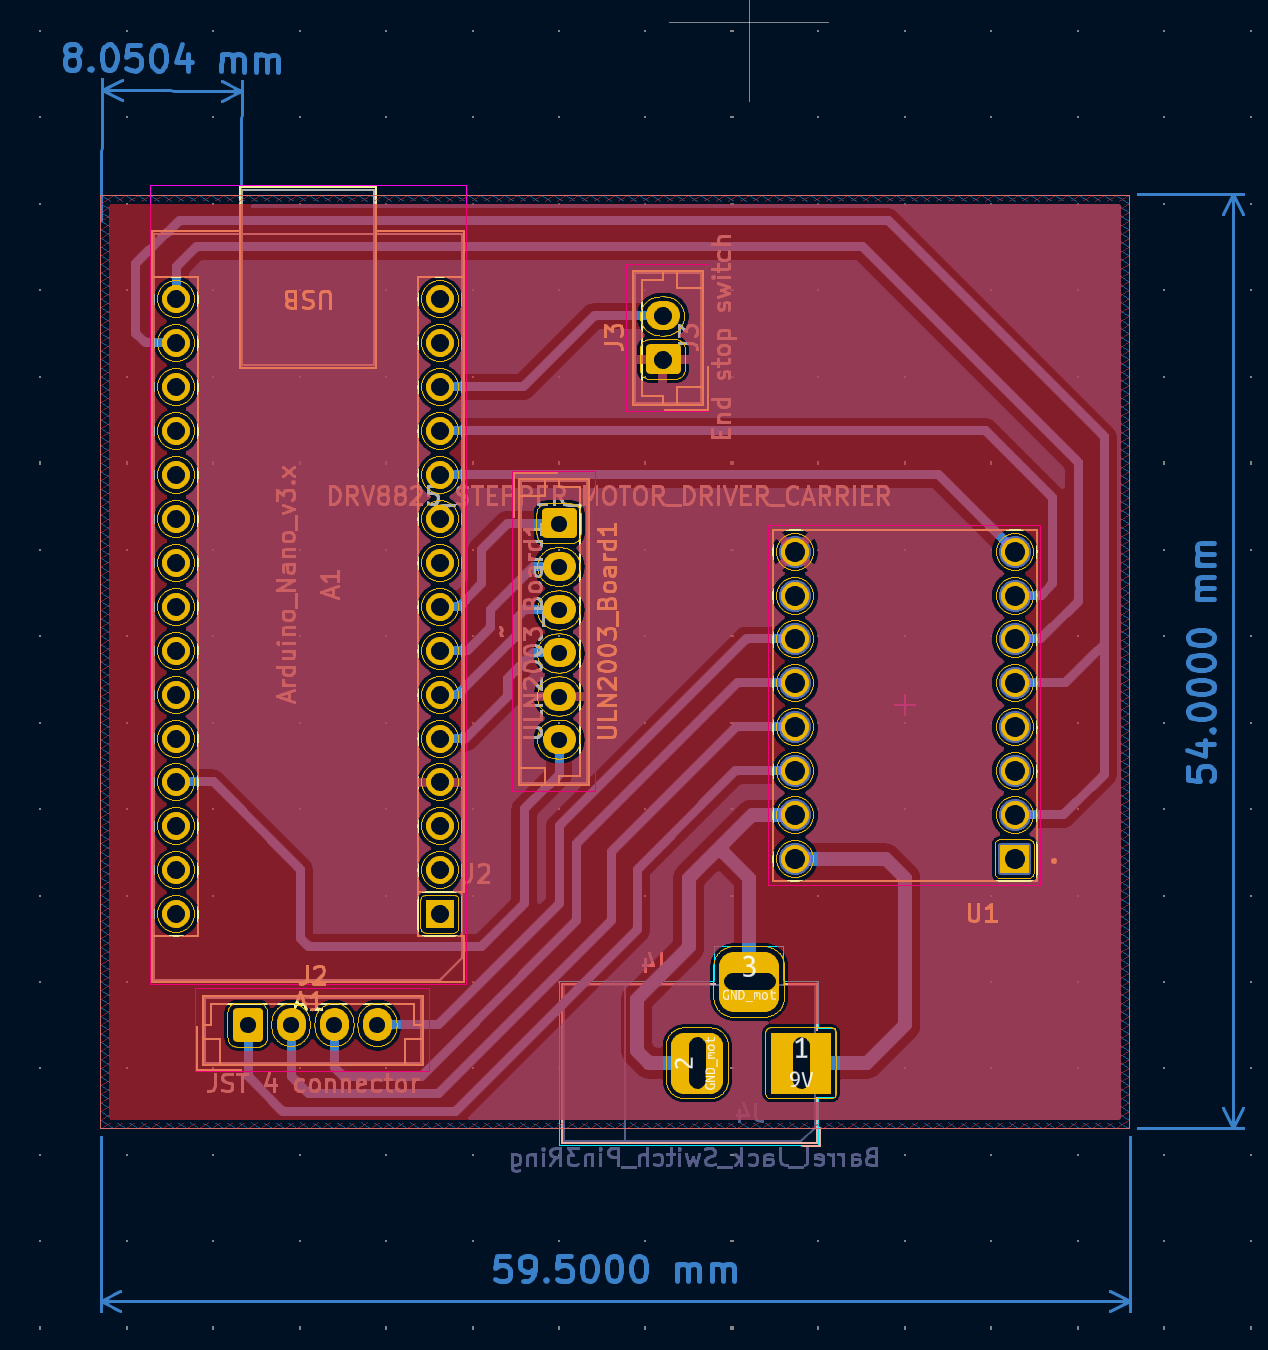
\includegraphics[width = \textwidth]{assets/figures/ameliorations/PCB_rotation_translation.png}
    \caption[PCB du système de mesure]{PCB du système de mesure (diagramme électrique disponible en \autoref{PCB:mesure})}
\end{figure}

\newpage
Le PCB réalisé au sein de l'école est populé de la façon suivante:

\begin{figure}[H]
    \centering
    \includegraphics[width = \textwidth]{assets/figures/ameliorations/PCB_mesure_Annoté.png}
    \caption[Photo du PCB du système de mesure]{Photo du PCB du système de mesure}
\end{figure}

La liste des pièces pour populer ce PCB est la suivante :
\begin{itemize}
    \item 1 - Arduino Nano - ici un Vellman WPB102
    \item 1 - switch de fin de course
    \item 1 - driver drv8825
    \item 1 - alimentation 9V
    \item 1 - Moteur 28byj-48 et sa board ULN2003
    \item 1 - Moteur 36H22HM-0404A15-Z
    \item 1 - connecteur femmelle JST 6 pin pas de 2.54mm
    \item 1 - Connecteur femelle JST 4 pin pas de 2.54mm
    \item 1 - Connecteur mâle cavalier 2 pin
\end{itemize}

À noter que le connecteur du moteur de translation possède un adaptateur, ceci est dû à une erreur de conception, cette erreur est corrigée
dans les fichiers fournis en annexe.

Concernant le driver drv 8825, il convient de régler la limite de courant que sera envoyée au moteur pas-à-pas, la marche à suivre est trouvable \href{https://www.pololu.com/product/2133}{ici}.\footnotemark

\footnotetext{\href{https://www.pololu.com/product/2133}{https://www.pololu.com/product/2133}}


\subsection{Machine de mesure}
Pour acceuillir le PCB et ses organes, il a donc fallu développer le système suivant :
\begin{figure}[H]
    \centering
    \includegraphics[width = \textwidth,trim={1cm 5cm 2cm 6cm},clip]{assets/figures/ameliorations/système_mesure_front.jpeg}
    \caption{Photo du système de mesure final}
\end{figure}

\newpage

\subsubsection{Fonctionnement}
Passons en revue le fonctionnement de la fonction de translation:
\begin{figure}[H]
    \centering
    \includegraphics[width = \textwidth]{assets/figures/ameliorations/3D_fonctionnement_crémaillère.png}
    \caption{Image du système de translation}
\end{figure}
La crémaillère est la partie fixe du système qui est reliée à la table optique, le pignon en tournant va alors décaler l'entièreté du système de mesure
vers la gauche ou la droite.

Le switch de fin de course sert à la fonction de homing du système, cela correspond à la position la plus à l'intérieur du disque
de phase pour le laser, en suite le système peut se déplacer sur une course de 4cm.

Concernant les resorts de compression, ils sont la pour assurer que la crémaillère ne "déraille" pas et que les dents du pignon rèstent bien plaquées
contre cette dernière, la plaque de pression est réglable en hauteur à l'aide de deux vis.

\newpage
\subsubsection{Réglage crémaillère}
\begin{figure}[H]
    \centering
    \includegraphics[width = \textwidth]{assets/figures/ameliorations/réglage_crémaillère_système_mesure.jpg}
    \caption{Réglage de la crémaillère lors du montage}
\end{figure}
Avant de fixer totalement le moteur du pignon, il faut bien veiller à ce que le système de crémaillère est bien réglé.
Comme on peut le voir sur la figure de gauche, il faut que le guide du support à crémaillère soit bien plaqué dans la rainure
de guidage du système de mesure, en suite comme sur l'image de droite, on peut alors régler la position verticale du pignon
pour que les dents de ce dernier et celle de la crémaillère soit bien en contact. Après cela, il conviendra d'ajuster la plaque de
pression pour bien maintenir le tout.

\subsubsection{Fixation de l'écran}
L'écran se fixe sur la machine de mesure à l'aide d'une vis à main :
\begin{figure}[H]
    \centering
    \includegraphics[width = \textwidth]{assets/figures/ameliorations/fixation_écran.png}
    \caption{Système de fixation de l'écran}
\end{figure}
À noter que les trous taraudés sont à faire à la main à l'aide d'un tourne à gauche directement dans le plastique, en effet,
cela est suffisement solide car l'utilisateur n'est pas censé démonter le moteur de rotation à chaque utilisation de la machine.

\subsubsection{Fixation du système de mesure au banc optique}
Le support à crémaillère vient se fixer sur un support de table optique à l'aide d'une vis sans tête m6 :
\begin{figure}[H]
    \centering
    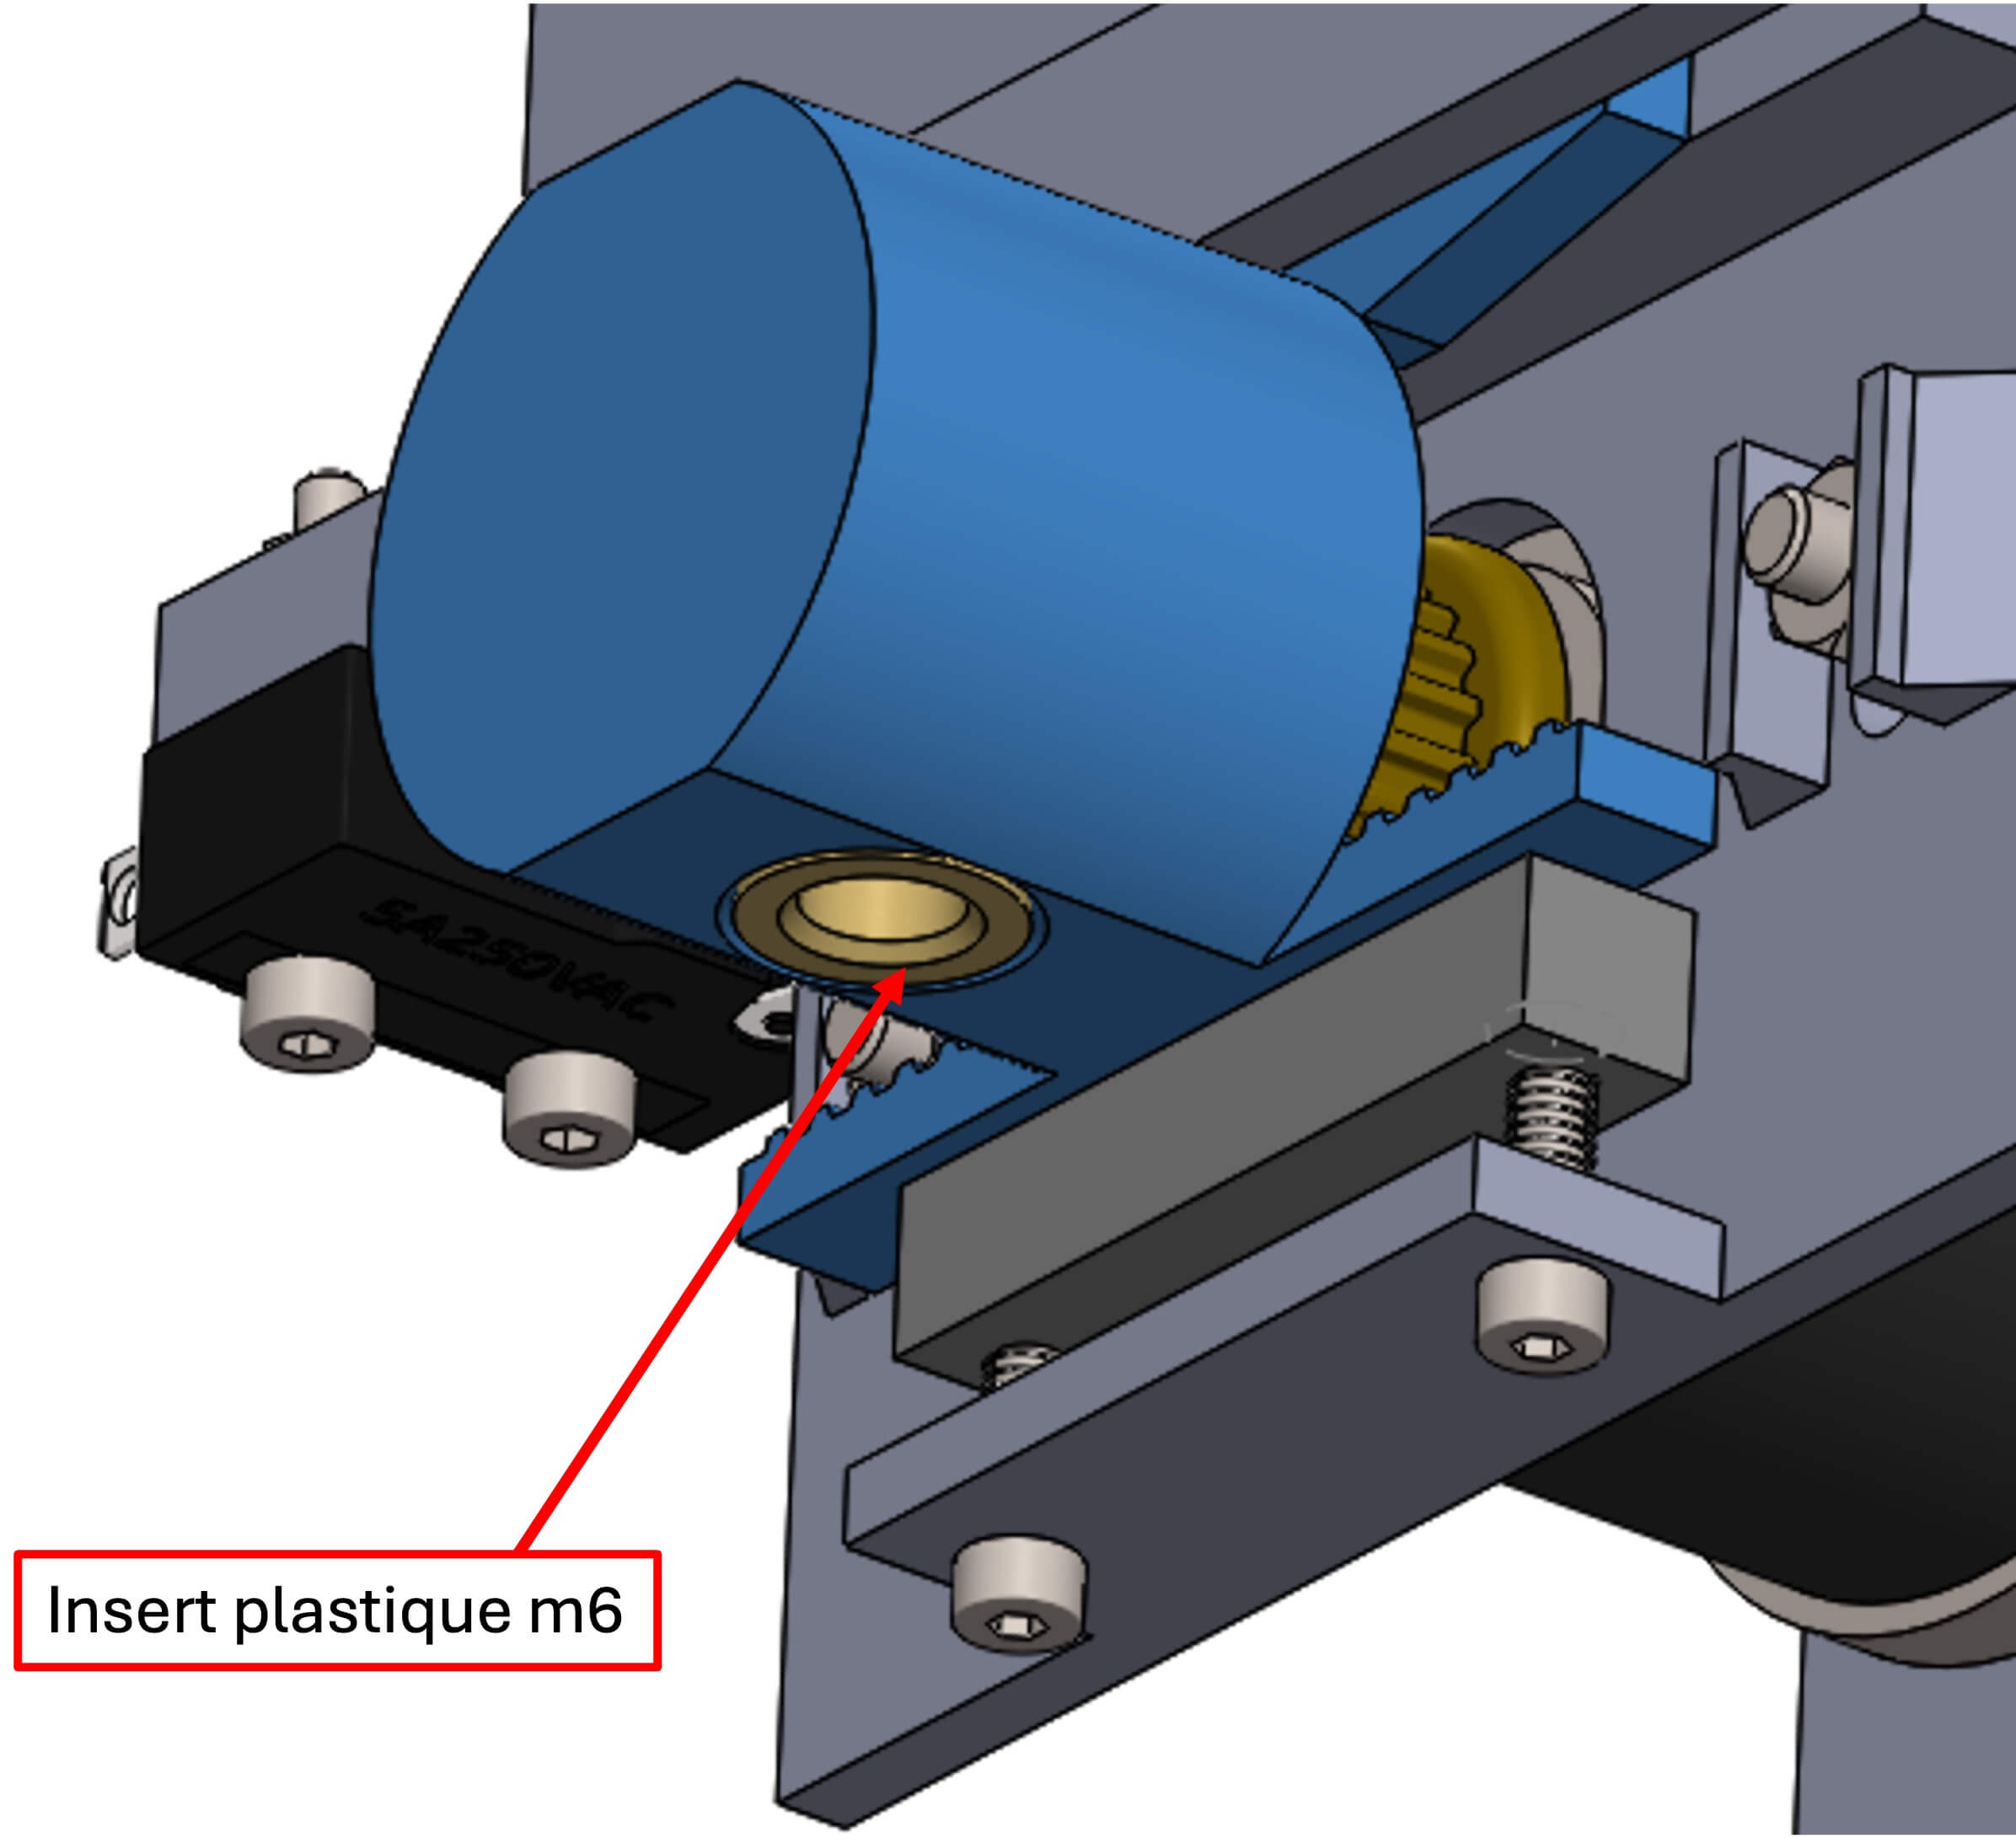
\includegraphics[width = 0.5\textwidth]{assets/figures/ameliorations/fixation_table_optique.jpg}
    \caption{Fixation du système de mesure à la table optique}
\end{figure}
\begin{figure}[H]
    \centering
    \includegraphics[width = 0.6\textwidth,trim = {0 2cm 3cm 3cm},clip]{assets/figures/ameliorations/système_mesure_back.jpeg}
    \caption{Photo du système sur un support de table optique}
\end{figure}

\newpage
\subsubsection{Fabrication du système de mesure}
Le système de mesure a été conçu avec l'impression 3D en tête, dans cette sous section, nous allons décrire quelques recommandation pour imprimer les pièces.
Pour la pièce principale, il est recommandé de l'imprimer dans cette orientation :

\begin{figure}[H]
    \centering
    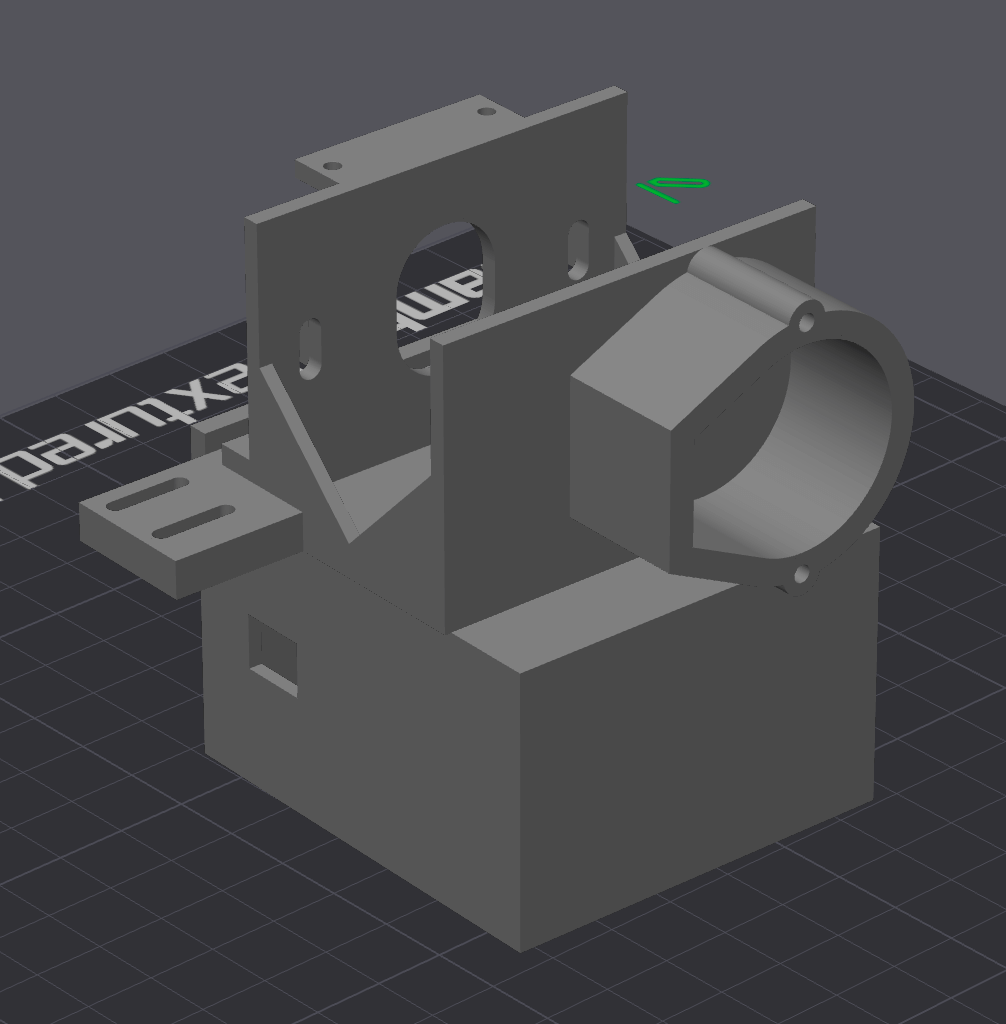
\includegraphics[width = 0.5\textwidth]{assets/figures/ameliorations/orientation_impression_systeme_mesure.png}
    \caption{Orientation d'impression système de mesure}
\end{figure}
Concernant les supports, il faut en mettre partout où il est nécessaire (c.f le projet BambuStudio donné en pièce jointes).

Pour le support à crémaillère l'orientation d'impression est la suivante :
\begin{figure}[H]
    \centering
    \includegraphics[width = 0.5\textwidth]{assets/figures/ameliorations/orientation_support_crémaillère.png}
    \caption{Orientation d'impression du support à crémaillère}
\end{figure}
Là aussi il conviendra de mettre des supports partout où il le faut !

\newpage
\subsection{Programme Matlab de mesure}
Comme dit précédemment, le programme pour réaliser les mesures des écrans a été réalisé sous Matlab à l'aide de la fonction "App Designer", l'interface est la suivante:
\begin{figure}[H]
    \centering
    \includegraphics[width = \textwidth]{assets/figures/ameliorations/capture interface.png}
    \caption{Interface programme de mesure}
\end{figure}
Pour fonctionner, le programme a besoin de :
\begin{itemize}
    \item l'addon matlab Arduino
    \item Du programme WFS de throlabs \cite{WFS_thorlabs_site}
    \item du fichier polzer.m
    \item du fichier indzer.m
    \item du fichier polzer\_array.mat
    \item du fichier thorlabswfs.m
\end{itemize}

Le fonctionnement du programme se base sur des boutons qui déclenchent des fonctions Callbacks, donc pas de boucle principale,
ni de fonctionnement séquentiel, dans cette section il conviendra donc d'expliquer le fonctionnement et la logique derrière le processus
de mesure, pour le reste le code source est normalement suffisement bien documenté.
\newpage

\section{Fabrication des écrans}
Comme dit dans la \autoref{sec:etat de lart}, la solution sera développée autour d'une buse d'atomisation pneumatique.
Cette dernière provient du fournisseur \href{https://www.spray.com/fr-eu}{Spraying Systems Co}\footnotemark.
Le model séléctionné est le corps de buse \textbf{B1/4JN-SS} et la tête de buse \textbf{SU1-SS } qui fournira une projection en cône plein.
\begin{figure}[H]
    \centering
    \includegraphics[width = 0.5\textwidth]{assets/figures/ameliorations/J_Series_1_8JN_and_1_4JN.jpeg}
    \caption[Buse B1/4JN-SS]{Buse B1/4JN-SS \cite{image_buse_spray_com}}
\end{figure}
Les raccords sur la le corps de la buse sont en BSPT 1/4 (donc 1/4 cônique), la buse est aussi équipée d'une aiguille de coupure manuelle du flux de liquide.
En partant donc de la machine originelle, le croquis de concept suivant a été développé:
\begin{figure}[H]
    \centering
    \includegraphics[width = 0.8\textwidth]{assets/figures/ameliorations/Croquis_machine_ecran_ver_1.png}
    \caption[Croquis nouvelle machine de spray ver. 1]{Croquis de la nouvelle machine de spray version 1}
\end{figure}

Cette buse est normalement capable de fonctionner uniquement avec de l'air comprimé qui créera une siphon aspirant le liquide à projeter d'une façon analogue à l'aérographe,
Malheureusement après des test préliminaires en connectant simplement la buse au système d'air de l'école et en essayant d'aspirer de l'eau, on a pu vite se rendre compte que la
configuration en siphon était problématique, en effet l'eau entrait dans la buse et était projetée une fraction de seconde avant d'être violement renvoyée dans le tuyaux d'entrée.
Il a fallu donc s'entretenir avec un conseillé de \textbf{Spraying System Co}, qui nous a donc conseillé d'utiliser une pompe péristaltique pour pousser le liquide dans la buse,
Aboutissant alors au second concept de la machine :
\begin{figure}[H]
    \centering
    \includegraphics[width = 0.9\textwidth]{assets/figures/ameliorations/Croquis_machine_ecran_ver_2.png}
    \caption[Croquis nouvelle machine de spray ver. 2]{Croquis de la nouvelle machine de spray version 2}
\end{figure}


\footnotetext{\href{https://www.spray.com/fr-eu}{https://www.spray.com/fr-eu}}

\chapter{Mesures}
\section{Écrans produits}
Plusieurs écrans exploitables ont été réalisés avec la nouvelle machine et l'ancienne machine pour les expositions suivantes au spray :
\begin{itemize}
    \item 5 secondes (ancienne machine + mesure manuelles)
    \item 10 secondes (ancienne machine + mesure manuelles)
    \item 15 secondes (nouvelle machine + mesure auto)
    \item 30 secondes (nouvelle machine + mesure auto)
    \item 60 secondes (nouvelle machine + mesure auto)
\end{itemize}
Par exploitables on entend qu'ils ressemblent visuellement au résultat attendu décrit dans la \autoref{sec:fab_ecran_sit_init}.
\begin{figure}[H]
    \centering
    \includegraphics[width = 0.5\textwidth]{assets/figures/mesures/15_sec.jpeg}
    \caption{Écran 15 secondes}
\end{figure}

\begin{figure}[H]
    \centering
    \includegraphics[width = 0.5\textwidth]{assets/figures/mesures/30_sec.jpeg}
    \caption{Écran 30 secondes}
\end{figure}

\begin{figure}[H]
    \centering
    \begin{subfigure}{.5\textwidth}
        \centering
        \includegraphics[width=1\linewidth]{assets/figures/mesures/60_sec.jpeg}
        \caption{Écran 60 secondes}
    \end{subfigure}%
    \begin{subfigure}{.5\textwidth}
        \centering
        \includegraphics[width=1\linewidth]{assets/figures/mesures/60_sec_travers.jpeg}
        \caption{Vue au travers de l'écran de 60 secondes}
    \end{subfigure}
    \caption{Écran 60 secondes de côté et au-travers}
\end{figure}
Sur l'écran on peut observer des défaut, il y a eut des problèmes de buse lors de cette projection, il sera toutefois
intéressant de caractériser cet écran. Le nombre de prise de mesure est à chaque fois de 100 mesures.

\section{Script d'analyse des données}
Le script d'analyse des données est dans un état assez brut, en effet pour analyser des données, il faudra rentrer manuellement
le chemin du répertoire des fichiers de données :
\begin{figure}[H]
    \centering
    \includegraphics[width = 1\textwidth]{assets/figures/mesures/exemple_chemin_fichier.png}
    \caption{Exemple de chemin de fichier}
\end{figure}
Il faut alors modifier les lignes en rose, avec les chemin des dossier contenant les .csv des mesures.

En suite il suffit de lancer l'exécution du script, ce dernier soustrait automatiquement les mesures de références
faites sans écrans à toutes les mesures des coefficients de Zernike, il calculera la variance de toutes les séries de mesures :
\begin{equation}
    var = \frac{1}{N-1}\sum_{j=1}^{N}|a_j - \mu|
\end{equation}
Où $\mu$ est la moyenne des coefficients de Zernike $a_j$
\begin{equation}
    \mu = \frac{1}{N}\sum_{j=1}^{N}a_j
\end{equation}
Dans le code cela donne :
\begin{figure}[H]
    \centering
    \includegraphics[width = 1\textwidth]{assets/figures/mesures/variance_matlab.png}
    \caption{Calcul de la variance des coefficients de Zernike}
\end{figure}
à la suite de ceci on obtient donc un tableau de dimension [1,66].

\newpage
En suite on utilise le fichier \textit{varianceNoll.m}, pour calculer les variances des coefficients de Zernike
pour $D/r_0 = 1$ :
\begin{figure}[H]
    \centering
    \includegraphics[width = 0.7\textwidth]{assets/figures/mesures/Calcul_variance_nool.png}
    \caption{Calcul des variances de Noll}
\end{figure}
En plottant les variances de Noll en fonction de leur indice j, à une échelle logarithmique, la courbe suivante est obtenue :
\begin{figure}[H]
    \centering
    \includegraphics[width = 0.7\textwidth]{assets/figures/mesures/plot_variance_Noll.png}
    \caption{Plot des variances de Noll}
\end{figure}
Ce plot est l'allure typique que nos mesures devraient suivre. Il représente les variances des coefficients de Zernike
des turbulences atmosphériques.

\newpage
Comme dit dans la théorie, selon l'\autoref{eq:param_fried}, convient maintenant de trouver le paramètre de Fried $r_0$
pour faire correspondre au mieux la courbe des mesures de l'écran et celle des valeurs théoriques :
\begin{figure}[H]
    \centering
    \includegraphics[width = 0.7\textwidth]{assets/figures/mesures/Noll_vs_mesure.png}
    \caption{Plot des variances de Noll vs Variance mesures}
\end{figure}

Pour se faire il conviendra de d'utiliser les fonctions \textit{fittype} et \textit{fit} pour trouver le $r_0$ qui convient le mieux :
\begin{figure}[H]
    \centering
    \includegraphics[width = 0.7\textwidth]{assets/figures/mesures/matlab_fit.png}
    \caption{Ligne du script pour fit le $r_0$}
\end{figure}
\color{red}/!\textbackslash \color{black}Dans le fit on exlu les 3 premiers coefficients de Zernike (Piston, inclinaison verticale, inclinaison horizontale),
en effet, ces 3 coefficients ne sont pas influencés par la turbulence mais par le système optique en lui même, ils ne sont donc pas relevant pour le fit.

La ligne commençant par \textbf{sigma\textunderscore fit} utilise l'\autoref{eq:param_fried}, où cette fois-ci on utilise le diamètre du diaphragme du système optique pour la
valeur de \textbf{D} ($\approx0.7 cm$). Une fois le fit effectué, il est possible de voir la valeur trouvée de $r_0$ dans la \textit{Command Window} de Matlab :
\begin{figure}[H]
    \centering
    \includegraphics[width = 0.7\textwidth]{assets/figures/mesures/fit_r_resultat.png}
    \caption{Exemple de $r_0$ trouvé par l'algorithme de fit}
\end{figure}

\newpage
Au final, le graph suivant est obtenu :
\begin{figure}[H]
    \centering
    \includegraphics[width = 1\textwidth]{assets/figures/mesures/Plot_final_avec_fit.png}
    \caption{Graph final avec variance Noll, variance mesures et variance fit}
\end{figure}

Dans une deuxième fenêtre, un histogramme de toutes les séries de mesures est affiché pour contrôler la distribution gaussienne de coefficients :
\begin{figure}[H]
    \centering
    \includegraphics[width = 0.6\textwidth]{assets/figures/mesures/histogramme_mesure.png}
    \caption{Histogramme de contrôle de la répartition des mesures}
\end{figure}

Le code du scipt d'analyse est disponible dans la \autoref{code:script_mesure_matlab}.

\newpage
\section{Résultats}
\subsection{Écran 15 secondes}
Plusieurs séries de mesures fûrent réalisées pour l'écran de 15 secondes :
\begin{figure}[H]
    \centering
    \includegraphics[width = 0.6\textwidth]{assets/figures/mesures/series_mesures_15sec.png}
    \caption{Séries de mesures écran 15 secondes}
\end{figure}
Les 3 premières séries ont étées réalisées à la suite avec les paramètres suivants :
\begin{itemize}
    \item Angle rotation : 3.6\textdegree
    \item Translation : 0mm
    \item Nombre de mesures : 100
\end{itemize}
Donc chaque séries se passe à exactement la même distance horizontale, commence et se finit à la même position angulaire.

La dernière série de mesure a été réalisée plus tôt pour tester le système de mesure.

\subsubsection{Mesure 15 secondes 1}
\begin{figure}[H]
    \centering
    \includegraphics[width = \textwidth]{assets/figures/mesures/mesure_15_sec_1_plot.png}
    \caption{Graphique de la série consécutive 1}
\end{figure}
Le \textbf{$r_0$} calculé est égal à : \textbf{0.006937 cm}.

\subsubsection{Mesure 15 secondes 2}
\begin{figure}[H]
    \centering
    \includegraphics[width = \textwidth]{assets/figures/mesures/mesure_15_sec_2_plot.png}
    \caption{Graphique de la série consécutive 2}
\end{figure}
Le \textbf{$r_0$} calculé est égal à : \textbf{0.03245 cm}.

\subsubsection{Mesure 15 secondes 3}
\begin{figure}[H]
    \centering
    \includegraphics[width = \textwidth]{assets/figures/mesures/mesure_15_sec_3_plot.png}
    \caption{Graphique de la série consécutive 3}
\end{figure}
Le \textbf{$r_0$} calculé est égal à : \textbf{0.01015 cm}.

\subsubsection{Mesure 15 secondes "écran\textunderscore15sec\textunderscore rota"}
\begin{figure}[H]
    \centering
    \includegraphics[width = \textwidth]{assets/figures/mesures/mesure_15_sec_rota_plot.png}
    \caption{Graphique de la série "écran\textunderscore15sec\textunderscore rota"}
\end{figure}
Le \textbf{$r_0$} calculé est égal à : \textbf{0.003195 cm}.

\subsection{Écran 30 secondes}
Ici une seule série de mesures avec les même paramètres que les écrans de 15 secondes a été réalisée :
\begin{figure}[H]
    \centering
    \includegraphics[width = 0.6\textwidth]{assets/figures/mesures/serie_mesures_30_sec_1.png}
    \caption{Série de mesures écran 30 secondes}
\end{figure}
Les deux autres séries ne contiennent que 10 mesures, ce qui n'est pas vraiment significatif pour tirer des conclusions.

\subsubsection{Mesure 30 secondes 1}
\begin{figure}[H]
    \centering
    \includegraphics[width = \textwidth]{assets/figures/mesures/mesure_30_sec_1_plot.png}
    \caption{Graphique de la série consécutive 1}
\end{figure}
Le \textbf{$r_0$} calculé est égal à : \textbf{0.001949 cm}.

\subsection{Écran 60 secondes}
Ici une seule série de mesure a été réalisée selon les mêmes paramètres cités précédemment :
\begin{figure}[H]
    \centering
    \includegraphics[width = 0.6\textwidth]{assets/figures/mesures/serie_mesures_60_sec.png}
    \caption{Série de mesures écran 60 secondes}
\end{figure}
\subsubsection{Mesure 60 secondes }
\begin{figure}[H]
    \centering
    \includegraphics[width = \textwidth]{assets/figures/mesures/mesure_60_sec_1_plot.png}
    \caption{Graphique de la série de mesure}
\end{figure}
Le \textbf{$r_0$} calculé est égal à : \textbf{0.001949 cm}.


\chapter{Conclusion}


\vfil
\hspace{8cm}\makeatletter\@author\makeatother\par
\hspace{8cm}\begin{minipage}{5cm}
    
\end{minipage}




\clearpage
%\bibliographystyle{plainnat}

\printbibliography

\appendix


\chapter{}
\newpage

\section[Fiche technique vernis Lascaux]{Fiche technique vernis Lascaux transparent 1-UV}\label{fiche_technique_Lascaux}

\begin{figure}[H]
    \centering
    \includepdf[pages=1,scale=0.9,pagecommand={}]{assets/Annexes/Lascaux Varnishes_Fixative.pdf}
    %\includegraphics[width = \textwidth]{assets/Annexes/chablon trous.pdf}
\end{figure}
\includepdf[pages=2-,scale=0.9,pagecommand={}]{assets/Annexes/Lascaux Varnishes_Fixative.pdf}

\section[Fiche technique Lascaux spécifique UV]{Fiche technique Lascaux spécifique UV}\label{fiche_technique_Lascaux_UV}

\begin{figure}[H]
    \centering
    \includepdf[pages=1,scale=0.9,pagecommand={}]{assets/Annexes/Lascaux_UV_Protect_E.pdf}
    %\includegraphics[width = \textwidth]{assets/Annexes/chablon trous.pdf}
\end{figure}
\includepdf[pages=2-,scale=0.9,pagecommand={}]{assets/Annexes/Lascaux_UV_Protect_E.pdf}


\section[Fiche technique Stardust Colors]{Fiche technique Top coats Stardust Colors}\label{fiche_technique_Stardust}

\begin{figure}[H]
    \centering
    \includepdf[pages=6,scale=0.7,angle=90,pagecommand={}]{assets/Annexes/Catalog_STARDUST PRO_UK.pdf}
    %\includegraphics[width = \textwidth]{assets/Annexes/chablon trous.pdf}
\end{figure}


\newpage
\section[Fiche technique vernis Createx]{Fiche technique vernis Createx}\label{fiche_technique_Createx}

\begin{figure}[H]
    \centering
    \includepdf[pages=1,scale=0.8,pagecommand={}]{assets/Annexes/UVLS-Clears-TDS.pdf}
    %\includegraphics[width = \textwidth]{assets/Annexes/chablon trous.pdf}
\end{figure}
\includepdf[pages=2-,scale=0.9,pagecommand={}]{assets/Annexes/UVLS-Clears-TDS.pdf}

\newpage
\section[Chablon trous vitre]{Chablon trous fixation vitre}\label{chablon_trous_vitre}

\begin{figure}[H]
    \centering
    \includepdf[pages=-,scale=1,pagecommand={}]{assets/Annexes/chablon trous.pdf}
    %\includegraphics[width = \textwidth]{assets/Annexes/chablon trous.pdf}
\end{figure}
\footnotetext{Télécharger fichiers source \href{https://1drv.ms/f/s!Altwa7Vt0GlIjv5WyyjY6xfEgrsDBQ?e=dFzJzf}{ici}}

\newpage
\section[Code arduino mesure]{Code arduino mesure \href{https://1drv.ms/f/s!Altwa7Vt0GlIj4Bf6049yvu0P-8YLQ?e=v7KWOI}{télécharger}}\label{code:arduino_mesure}
\lstinputlisting[language=Arduino]{assets/code/Code_arduino_mesure.ino}
\footnotetext{Télécharger fichiers source \href{https://1drv.ms/f/s!Altwa7Vt0GlIj4Bf6049yvu0P-8YLQ?e=v7KWOI}{ici}}


\section[Diagramme électrique PCB mesure]{Diagramme électrique PCB mesure\href{https://1drv.ms/f/s!Altwa7Vt0GlIjv0bGlDjWqrtS53P8w?e=SVTypX}{Télécharger}}\label{PCB:mesure}
\begin{figure}[H]
    \centering
    \includegraphics[angle = 90,height = 0.8\paperheight]{assets/Annexes/PCB_rotation_translation_diagramme_elec.pdf}
    %\includepdf[pages=-,scale=1,angle = 90,pagecommand={}]{assets/Annexes/PCB_rotation_translation_diagramme_elec.pdf}
    %\includegraphics[width = \textwidth]{assets/Annexes/chablon trous.pdf}
\end{figure}

\section[Mise en plan Système de mesure]{Mise en plan Système de mesure}\label{mise_en_plan_systeme_mesure}

\begin{figure}[H]
    \centering
    \includepdf[pages=-,scale=0.7,angle = 90,pagecommand={}]{assets/Annexes/assemblage_machine_mesure.pdf}
    %\includegraphics[width = \textwidth]{assets/Annexes/chablon trous.pdf}
\end{figure}


\section[Diagramme électrique PCB machine spray]{Diagramme électrique PCB machine spray\href{https://1drv.ms/b/s!Altwa7Vt0GlIj55oN6zv-TJly9lecA?e=SIccNb}{Télécharger}}\label{PCB:spray}
\begin{figure}[H]
    \centering
    \includegraphics[angle = 90,height = 0.8\paperheight]{assets/Annexes/Diagramme_PCB_spray.pdf}
    %\includepdf[pages=-,scale=1,angle = 90,pagecommand={}]{assets/Annexes/PCB_rotation_translation_diagramme_elec.pdf}
    %\includegraphics[width = \textwidth]{assets/Annexes/chablon trous.pdf}
\end{figure}
\addappheadtotoc



\let\cleardoublepage\clearpage
\backmatter

\label{glossaire}
\printnoidxglossary
\label{index}
\printindex

% Le colophon est le dernier élément d'un document qui contient des notes de l'auteur concernant la mise en page et l'édition du document : il est parfaitement optionnel.
\input{colophon.tex}

\end{document}
